\documentclass[12pt]{beamer}
\usepackage[english]{babel}
\usepackage{datetime}
\usepackage{tikz}
\usetikzlibrary{shapes.geometric}
\usetikzlibrary{matrix}
\usepackage{animate}
\usepackage{color}
\usepackage{colortbl}
\usepackage{graphicx}
\usepackage{ifthen}
\usetheme{Berlin}

\title[Employer Search and Screening in an Online Labor Market]{Employer Search and\\Screening in an Online\\Labor Market}
\author{John J. Horton}
\institute{oDesk Research}

\setbeamertemplate{footline}{%
  \begin{beamercolorbox}[sep=1mm,wd=\paperwidth,leftskip=1mm,rightskip=1mm]{footlinecolor}
    \hspace{1mm}%
    \tiny{\insertdate}
    \hfill
  \end{beamercolorbox}%
}

%gets rid of navigation symbols
\setbeamertemplate{navigation symbols}{}

\tikzstyle{every picture}+=[remember picture]
\tikzstyle{na} = [baseline=-.5ex]

\definecolor{myred}{RGB}{200,0,0}
\definecolor{mygreen}{RGB}{0,200,0}
\definecolor{myyellow}{RGB}{230,230,0}
\definecolor{gray100}{RGB}{0,0,0}
\definecolor{gray75}{RGB}{64,64,64}
\definecolor{gray50}{RGB}{128,128,128}
\definecolor{gray25}{RGB}{192,192,192}
\definecolor{gray0}{RGB}{255,255,255}
\definecolor{red100}{RGB}{255,0,0}
\definecolor{red75}{RGB}{255,64,64}
\definecolor{red50}{RGB}{255,128,128}
\definecolor{red25}{RGB}{255,192,192}
\definecolor{red0}{RGB}{255,255,255}
\definecolor{yellow100}{RGB}{255,255,0}
\definecolor{yellow75}{RGB}{255,255,64}
\definecolor{yellow50}{RGB}{255,255,128}
\definecolor{yellow25}{RGB}{255,255,192}
\definecolor{yellow0}{RGB}{255,255,255}

\newcolumntype{C}[1]{>{\centering}m{#1}}

%our imaginary items - that is, placeholders for items
\newcommand*\imgitem{%
\item[\color{white}\scalebox{0.9}{\textbullet}]}

\newcommand*\imgitemtf{%
\item[\color{gray25}\scalebox{0.9}{\textbullet}]}

\newcommand*\imgitemfo{%
\item[\color{gray50}\scalebox{0.9}{\textbullet}]}

\newcommand*\imgitemsf{%
\item[\color{gray75}\scalebox{0.9}{\textbullet}]}

%our items
\newcommand*\ouritem{%
\item[\color{black}\scalebox{0.9}{\textbullet}]}

%our items
\newcommand*\variitem[1]{%
\item[\color{#1}\scalebox{0.9}{\textbullet}]}

\newcommand\redbox[3]{%
\begin{tikzpicture}[remember picture,overlay]
  \node[rectangle,rounded corners,line width=1pt,
      draw=myred,fill=myred!30,text height=20pt,
      text depth=11pt,align=left,fill opacity=0.7,text opacity=1] 
    (boxred) at #3 {#2};
  \node[rectangle,rounded corners,fill=myred!90,
      font={\Large\color{white}},anchor=west] 
    at ([xshift=10pt,]boxred.north west) {#1};
\end{tikzpicture}%
}

\newcommand\invbox[2]{%
\begin{tikzpicture}[remember picture,overlay]
  \node 
    (boxinv) at #2 {#1};
\end{tikzpicture}%
}

\newcommand\colorstar[1]{
\tikzstyle{scorestars}=[star, star points=5, star point ratio=2.25, draw,inner sep=1.3pt,anchor=outer point 3]
  \begin{tikzpicture}[baseline]
    \draw (0,0) node[name=star,scorestars,fill=yellow#1,draw=gray#1]  {};
  \end{tikzpicture}
}

\newcommand\ministar[1]{
\tikzstyle{scorestars}=[star, star points=5, star point ratio=2.25, draw,inner sep=0.9pt]
  \begin{tikzpicture}[baseline]
    \draw (0,0) node[shift={(-0.7,0.05)},name=ministar,scorestars,fill=yellow#1,draw=gray#1]  {};
  \end{tikzpicture}
}

\def\mytemparray{}

%
\newcommand\doatpos[2]{%
    \bgroup
    \def\mytemparray{{ #1 }}
    \pgfmathparse{\mytemparray[0]} \edef\mya{\pgfmathresult}
    \pgfmathparse{\mytemparray[1]} \edef\myb{\pgfmathresult}
    \pgfmathparse{\mytemparray[2]} \edef\myc{\pgfmathresult}
    \begin{tikzpicture}[remember picture, overlay]
            \node[opacity=\myc] at ( \mya pt, \myb  pt) {#2};
    \end{tikzpicture}%
        %
    %
    \egroup
%
}

\newcommand\putat[3]{%
    \bgroup
    \pgfmathparse{#1 \textwidth} \edef\mya{\pgfmathresult}
    \pgfmathparse{- #2 \textheight} \edef\myb{\pgfmathresult}
    \begin{tikzpicture}[remember picture, overlay]
            \node at ( \mya pt, \myb  pt) {#3};
    \end{tikzpicture}%
        %
    %
    \egroup
%
}

\newcommand\putattrans[4]{%
    \bgroup
    \pgfmathparse{#1 \textwidth} \edef\mya{\pgfmathresult}
    \pgfmathparse{- #2 \textheight} \edef\myb{\pgfmathresult}
    \begin{tikzpicture}[remember picture, overlay]
            \node[text opacity=#3] at ( \mya pt, \myb  pt) {#4};
    \end{tikzpicture}%
        %
    %
    \egroup
%
}

%posx, posy, boxcolor, textcolor, text
\newcommand\boxat[5]{%
    \bgroup
    \pgfmathparse{#1 \textwidth} \edef\mya{\pgfmathresult}
    \pgfmathparse{- #2 \textheight} \edef\myb{\pgfmathresult}
    \begin{tikzpicture}[remember picture,overlay]
         \node[rectangle,rounded corners,line width=1pt,
         draw=#3,fill=#3!30,text height=6pt,font={\color{#4}},
         text depth=0pt,align=center,fill opacity=0.7,text opacity=1] 
         (boxred) at ( \mya pt, \myb  pt) {\phantom{#5}};
         \node[rectangle,rounded corners,line width=1pt,
         draw=#3,fill=#3!30,text height=6pt,font={\color{#4}},
         text depth=0pt,align=center,draw opacity=0,fill opacity=0,text opacity=1,shift={(1pt,0)}] 
         (boxred) at ( \mya pt, \myb  pt) {#5};
\end{tikzpicture}%
        %
    %
    \egroup
%
}

%posx, posy, boxcolor, textcolor, text
\newcommand\bigboxat[5]{%
    \bgroup
    \pgfmathparse{#1 \textwidth} \edef\mya{\pgfmathresult}
    \pgfmathparse{- #2 \textheight} \edef\myb{\pgfmathresult}
    \begin{tikzpicture}[remember picture,overlay]
         \node[rectangle,rounded corners,line width=1pt,
         draw=#3,fill=#3!30,text height=30pt,font={\color{#4}},
         text depth=11pt,align=left,fill opacity=0.7,text opacity=1] 
         (boxred) at ( \mya pt, \myb  pt) {#5};
\end{tikzpicture}%
        %
    %
    \egroup
%
}

\begin{document}

\setlength{\baselineskip}{12mm}
\fontsize{10mm}{12mm}\selectfont

\begin{frame}
\begin{center}
Employer Search and\\
Screening in an Online\\
Labor Market

\vspace{3mm}

\large
John J. Horton\\
oDesk Research
\end{center}
\end{frame}

\begin{frame}{}
\begin{animateinline}[autoplay]{10}
\multiframe{5}{i=0+25}{
\begin{minipage}{\textwidth}
\begin{center}
\vspace{1mm}

\textcolor{gray\i}{Matching markets have}

\textcolor{gray\i}{search screening costs}

\vspace{1mm}
\end{center}
\end{minipage}
}
\end{animateinline}
\end{frame}

\begin{frame}{}
\begin{animateinline}[autoplay]{10}
\multiframe{5}{i=0+25}{
\begin{minipage}{\textwidth}
\Large
\begin{itemize}
\variitem{gray\i} \textcolor{gray\i}{What \emph{are} my options?}

\imgitem \textcolor{white}{\emph{How good} is each option for me?}
\end{itemize}
\end{minipage}
}
\newframe
\multiframe{5}{i=0+25}{
\begin{minipage}{\textwidth}
\Large
\begin{itemize}
\ouritem What \emph{are} my options?

\variitem{gray\i} \textcolor{gray\i}{\emph{How good} is each option for me?}
\end{itemize}
\end{minipage}
}
\end{animateinline}
\end{frame}

\begin{frame}{}
\begin{animateinline}[autoplay]{10}
\multiframe{5}{i=0+25}{
\begin{minipage}[c]{1\textwidth}
\begin{center}
\Large

\begin{figure}[H] \centering 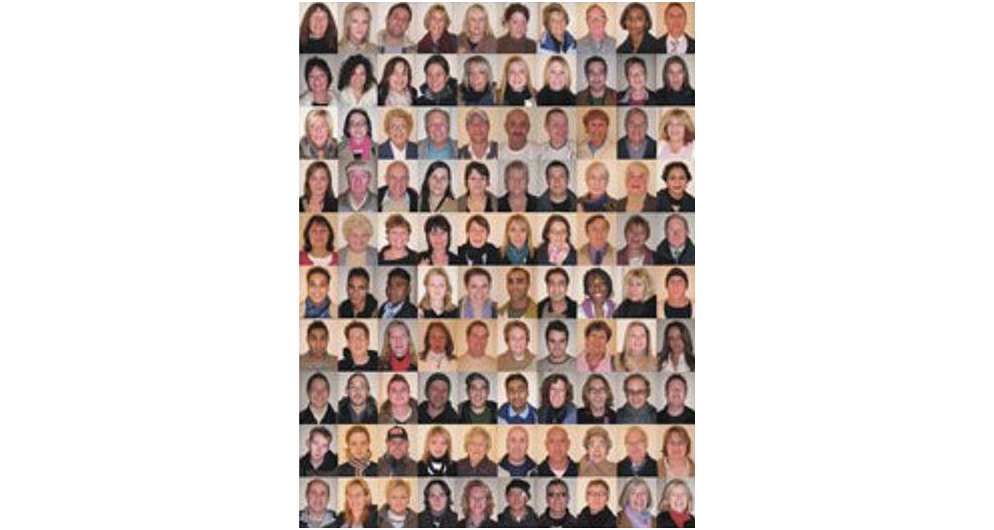
\includegraphics[width=100mm]{people_animation_1.png} \end{figure}

\textcolor{gray\i}{100 people}
\end{center}
\end{minipage}
}
\end{animateinline}
\end{frame}

\begin{frame}{}
\begin{animateinline}[autoplay]{10}
\multiframe{11}{i=1+1}{
\begin{minipage}[c]{1\textwidth}
\begin{center}
\Large

\begin{figure}[H] \centering \includegraphics[width=100mm]{people_animation_\i.png} \end{figure}

100 people
\end{center}
\end{minipage}
}
\newframe
\multiframe{9}{i=11+1}{
\begin{minipage}[c]{1\textwidth}
\begin{center}
\Large

\begin{figure}[H] \centering \includegraphics[width=100mm]{people_animation_\i.png} \end{figure}

1,000 people
\end{center}
\end{minipage}
}
\end{animateinline}
\end{frame}

\begin{frame}{}
\begin{animateinline}[autoplay]{10}
\multiframe{5}{i=1+1}{
\begin{minipage}[c]{1\textwidth}
\begin{center}
\Large

\begin{figure}[H] \centering \includegraphics[width=100mm]{people_animation_2_\i.png} \end{figure}

1,000 people
\end{center}
\end{minipage}
}
\newframe
\multiframe{6}{i=6+1}{
\begin{minipage}[c]{1\textwidth}
\begin{center}
\Large

\begin{figure}[H] \centering \includegraphics[width=100mm]{people_animation_2_\i.png} \end{figure}

100,000 people
\end{center}
\end{minipage}
}
\end{animateinline}
\end{frame}

\begin{frame}{}
\begin{animateinline}[autoplay]{10}
\multiframe{10}{i=1+1}{
\begin{minipage}[c]{1\textwidth}
\begin{center}
\Large

\begin{figure}[H] \centering \includegraphics[width=100mm]{people_animation_3_\i.png} \end{figure}

100,000 people
\end{center}
\end{minipage}
}
\newframe
\multiframe{8}{i=11+1}{
\begin{minipage}[c]{1\textwidth}
\begin{center}
\Large

\begin{figure}[H] \centering \includegraphics[width=100mm]{people_animation_3_\i.png} \end{figure}

1,000,000 people
\end{center}
\end{minipage}
}
\end{animateinline}
\end{frame}

\begin{frame}{}
\begin{animateinline}[autoplay]{10}
\multiframe{5}{i=0+25}{
\begin{minipage}{\textwidth}
\vspace{1 mm}
\begin{center}
\textcolor{gray\i}{Algorithmic approach}
\end{center}

\Large
\begin{itemize}
\imgitem \textcolor{white}{Infer nature of the work}

\imgitem \textcolor{white}{Find candidates with matching skills}

\imgitem \textcolor{white}{Sort matching candidates by some weighted combination of ability \& availability}
\end{itemize}
\end{minipage}
}
\newframe
\multiframe{5}{i=0+25}{
\begin{minipage}{\textwidth}
\vspace{1 mm}
\begin{center}
Algorithmic approach
\end{center}

\Large
\begin{itemize}
\variitem{gray\i} \textcolor{gray\i}{Infer nature of the work}

\imgitem \textcolor{white}{Find candidates with matching skills}

\imgitem \textcolor{white}{Sort matching candidates by some weighted combination of ability \& availability}
\end{itemize}
\end{minipage}
}
\newframe
\multiframe{5}{i=0+25}{
\begin{minipage}{\textwidth}
\vspace{1 mm}
\begin{center}
Algorithmic approach
\end{center}

\Large
\begin{itemize}
\ouritem Infer nature of the work

\variitem{gray\i} \textcolor{gray\i}{Find candidates with matching skills}

\imgitem \textcolor{white}{Sort matching candidates by some weighted combination of ability \& availability}
\end{itemize}
\end{minipage}
}
\newframe
\multiframe{5}{i=0+25}{
\begin{minipage}{\textwidth}
\vspace{1 mm}
\begin{center}
Algorithmic approach
\end{center}

\Large
\begin{itemize}
\ouritem Infer nature of the work

\ouritem Find candidates with matching skills

\variitem{gray\i} \textcolor{gray\i}{Sort matching candidates by some weighted combination of ability \& availability}
\end{itemize}
\end{minipage}
}
\end{animateinline}
\end{frame}

\begin{frame}{}
\begin{animateinline}[autoplay]{10}
\multiframe{5}{i=0+25}{
\begin{minipage}{\textwidth}
\vspace{1 mm}
\begin{center}
\textcolor{gray\i}{What segments matching}

\textcolor{gray\i}{markets traditionally?}
\end{center}

\Large
\begin{itemize}
\imgitem \textcolor{white}{Geography}

\imgitem \textcolor{white}{Time}

\imgitem \textcolor{white}{Costs of application}
\end{itemize}

\nointerlineskip
\begin{tikzpicture}[overlay]
\end{tikzpicture}
\end{minipage}
}
\newframe
\multiframe{5}{i=0+25}{
\begin{minipage}{\textwidth}
\vspace{1 mm}
\begin{center}
What segments matching

markets traditionally?
\end{center}

\Large
\begin{itemize}
\variitem{gray\i} \textcolor{gray\i}{Geography}

\imgitem \textcolor{white}{Time}

\imgitem \textcolor{white}{Costs of application}
\end{itemize}

\nointerlineskip
\begin{tikzpicture}[overlay]
\end{tikzpicture}
\end{minipage}
}
\newframe
\multiframe{5}{i=0+25}{
\begin{minipage}{\textwidth}
\vspace{1 mm}
\begin{center}
What segments matching

markets traditionally?
\end{center}

\Large
\begin{itemize}
\ouritem Geography

\variitem{gray\i} \textcolor{gray\i}{Time}

\imgitem \textcolor{white}{Costs of application}
\end{itemize}

\nointerlineskip
\begin{tikzpicture}[overlay]
\end{tikzpicture}
\end{minipage}
}
\newframe
\multiframe{5}{i=0+25}{
\begin{minipage}{\textwidth}
\vspace{1 mm}
\begin{center}
What segments matching

markets traditionally?
\end{center}

\Large
\begin{itemize}
\ouritem Geography

\ouritem Time

\variitem{gray\i} \textcolor{gray\i}{Costs of application}
\end{itemize}

\nointerlineskip
\begin{tikzpicture}[overlay]
\end{tikzpicture}
\end{minipage}
}
\newframe[20]
\begin{minipage}{\textwidth}
\vspace{1 mm}
\begin{center}
What segments matching

markets traditionally?
\end{center}

\Large
\begin{itemize}
\ouritem \tikz[na] \node[coordinate] (geo1) {};G\tikz[na] \node[coordinate] (geo2) {};eography

\ouritem Time

\ouritem Costs of application
\end{itemize}

\nointerlineskip
\begin{tikzpicture}[overlay]
\draw[line width=2pt,red] (geo1) edge [out=0, in=180] (geo2);
\end{tikzpicture}
\end{minipage}
\newframe
\begin{minipage}{\textwidth}
\vspace{1 mm}
\begin{center}
What segments matching

markets traditionally?
\end{center}

\Large
\begin{itemize}
\ouritem \tikz[na] \node[coordinate] (geo1) {};Ge\tikz[na] \node[coordinate] (geo2) {};ography

\ouritem Time

\ouritem Costs of application
\end{itemize}

\nointerlineskip
\begin{tikzpicture}[overlay]
\draw[line width=2pt,red] (geo1) edge [out=0, in=180] (geo2);
\end{tikzpicture}
\end{minipage}
\newframe
\begin{minipage}{\textwidth}
\vspace{1 mm}
\begin{center}
What segments matching

markets traditionally?
\end{center}

\Large
\begin{itemize}
\ouritem \tikz[na] \node[coordinate] (geo1) {};Geo\tikz[na] \node[coordinate] (geo2) {};graphy

\ouritem Time

\ouritem Costs of application
\end{itemize}

\nointerlineskip
\begin{tikzpicture}[overlay]
\draw[line width=2pt,red] (geo1) edge [out=0, in=180] (geo2);
\end{tikzpicture}
\end{minipage}
\newframe
\begin{minipage}{\textwidth}
\vspace{1 mm}
\begin{center}
What segments matching

markets traditionally?
\end{center}

\Large
\begin{itemize}
\ouritem \tikz[na] \node[coordinate] (geo1) {};Geog\tikz[na] \node[coordinate] (geo2) {};raphy

\ouritem Time

\ouritem Costs of application
\end{itemize}

\nointerlineskip
\begin{tikzpicture}[overlay]
\draw[line width=2pt,red] (geo1) edge [out=0, in=180] (geo2);
\end{tikzpicture}
\end{minipage}
\newframe
\begin{minipage}{\textwidth}
\vspace{1 mm}
\begin{center}
What segments matching

markets traditionally?
\end{center}

\Large
\begin{itemize}
\ouritem \tikz[na] \node[coordinate] (geo1) {};Geogr\tikz[na] \node[coordinate] (geo2) {};aphy

\ouritem Time

\ouritem Costs of application
\end{itemize}

\nointerlineskip
\begin{tikzpicture}[overlay]
\draw[line width=2pt,red] (geo1) edge [out=0, in=180] (geo2);
\end{tikzpicture}
\end{minipage}
\newframe
\begin{minipage}{\textwidth}
\vspace{1 mm}
\begin{center}
What segments matching

markets traditionally?
\end{center}

\Large
\begin{itemize}
\ouritem \tikz[na] \node[coordinate] (geo1) {};Geogra\tikz[na] \node[coordinate] (geo2) {};phy

\ouritem Time

\ouritem Costs of application
\end{itemize}

\nointerlineskip
\begin{tikzpicture}[overlay]
\draw[line width=2pt,red] (geo1) edge [out=0, in=180] (geo2);
\end{tikzpicture}
\end{minipage}
\newframe
\begin{minipage}{\textwidth}
\vspace{1 mm}
\begin{center}
What segments matching

markets traditionally?
\end{center}

\Large
\begin{itemize}
\ouritem \tikz[na] \node[coordinate] (geo1) {};Geograp\tikz[na] \node[coordinate] (geo2) {};hy

\ouritem Time

\ouritem Costs of application
\end{itemize}

\nointerlineskip
\begin{tikzpicture}[overlay]
\draw[line width=2pt,red] (geo1) edge [out=0, in=180] (geo2);
\end{tikzpicture}
\end{minipage}
\newframe
\begin{minipage}{\textwidth}
\vspace{1 mm}
\begin{center}
What segments matching

markets traditionally?
\end{center}

\Large
\begin{itemize}
\ouritem \tikz[na] \node[coordinate] (geo1) {};Geograph\tikz[na] \node[coordinate] (geo2) {};y

\ouritem Time

\ouritem Costs of application
\end{itemize}

\nointerlineskip
\begin{tikzpicture}[overlay]
\draw[line width=2pt,red] (geo1) edge [out=0, in=180] (geo2);
\end{tikzpicture}
\end{minipage}
\newframe
\begin{minipage}{\textwidth}
\vspace{1 mm}
\begin{center}
What segments matching

markets traditionally?
\end{center}

\Large
\begin{itemize}
\ouritem \tikz[na] \node[coordinate] (geo1) {};Geography\tikz[na] \node[coordinate] (geo2) {};

\ouritem Time

\ouritem Costs of application
\end{itemize}

\nointerlineskip
\begin{tikzpicture}[overlay]
\draw[line width=2pt,red] (geo1) edge [out=0, in=180] (geo2);
\end{tikzpicture}
\end{minipage}
\newframe[10]
\multiframe{5}{i=0+25}{
\begin{minipage}{\textwidth}
\vspace{1 mm}
\begin{center}
What segments matching

markets traditionally?
\end{center}

\Large
\begin{itemize}
\ouritem \tikz[na] \node[coordinate] (geo1) {};Geography\tikz[na] \node[coordinate] (geo2) {}; 
\invbox{
\small
\textcolor{red\i}{No inherent geographic constraints}}{(0.3\textwidth,0.025\textheight)}
\invbox{
\small
\textcolor{red\i}{in online labor markets}}{(0.3\textwidth,-0.025\textheight)}

\ouritem Time

\ouritem Costs of application
\end{itemize}

\nointerlineskip
\begin{tikzpicture}[overlay]
\draw[line width=2pt,red] (geo1) edge [out=0, in=180] (geo2);
\end{tikzpicture}
\end{minipage}
}
\end{animateinline}
\end{frame}

\begin{frame}{}
\begin{animateinline}[autoplay]{10}
\multiframe{5}{i=0+25}{
\begin{minipage}{\textwidth}
\vspace{1 mm}
\begin{center}
\textcolor{gray\i}{Search and scale}
\end{center}

\Large
\begin{itemize}
\imgitem \textcolor{white}{Effects of scale}

\begin{itemize}
\Large
\imgitem \textcolor{white}{Plus: More space for higher-quality matches}

\imgitem \textcolor{white}{Negative: The {\grqq}what are'' and {\grqq}how good are'' questions about options get harder with scale}
\end{itemize}
\end{itemize}
\end{minipage}
}
\newframe
\multiframe{5}{i=0+25}{
\begin{minipage}{\textwidth}
\vspace{1 mm}
\begin{center}
Search and scale
\end{center}

\Large
\begin{itemize}
\variitem{gray\i} \textcolor{gray\i}{Effects of scale}

\begin{itemize}
\Large
\imgitem \textcolor{white}{Plus: More space for higher-quality matches}

\imgitem \textcolor{white}{Negative: The {\grqq}what are'' and {\grqq}how good are'' questions about options get harder with scale}
\end{itemize}
\end{itemize}
\end{minipage}
}
\newframe
\multiframe{5}{i=0+25}{
\begin{minipage}{\textwidth}
\vspace{1 mm}
\begin{center}
Search and scale
\end{center}

\Large
\begin{itemize}
\ouritem Effects of scale

\begin{itemize}
\Large
\variitem{gray\i} \textcolor{gray\i}{Plus: More space for higher-quality matches}

\imgitem \textcolor{white}{Negative: The {\grqq}what are'' and {\grqq}how good are'' questions about options get harder with scale}
\end{itemize}
\end{itemize}
\end{minipage}
}
\newframe
\multiframe{5}{i=0+25}{
\begin{minipage}{\textwidth}
\vspace{1 mm}
\begin{center}
Search and scale
\end{center}

\Large
\begin{itemize}
\ouritem Effects of scale

\begin{itemize}
\Large
\ouritem Plus: More space for higher-quality matches

\variitem{gray\i} \textcolor{gray\i}{Negative: The {\grqq}what are'' and {\grqq}how good are'' questions about options get harder with scale}
\end{itemize}
\end{itemize}
\end{minipage}
}
\end{animateinline}
\end{frame}

\begin{frame}{}
\begin{animateinline}[autoplay]{10}
\multiframe{5}{i=0+25}{
\begin{minipage}{\textwidth}
\Large
\vspace{1 mm}
\begin{itemize}
\variitem{gray\i} \textcolor{gray\i}{To what extent can we subsidize search and screening algorithmically, and is this subsidization effective?}
\end{itemize}
\end{minipage}
}
\end{animateinline}
\end{frame}

\begin{frame}{}
\begin{animateinline}[autoplay]{10}
\multiframe{5}{i=0+25}{
\begin{minipage}{\textwidth}
\begin{center}
\vspace{1 mm}
\textcolor{gray\i}{Can these costs be reduced by third-parties?}
\end{center}
\end{minipage}
}
\end{animateinline}
\end{frame}

\begin{frame}{}
\begin{animateinline}[autoplay]{10}
\multiframe{5}{i=0+25}{
\begin{minipage}{\textwidth}
\begin{center}
\textcolor{gray\i}{Labor market examples}
\end{center}

\Large
\vspace{1 mm}
\begin{itemize}
\imgitem \textcolor{white}{Credentialing services}

\imgitem \textcolor{white}{Unions}

\imgitem \textcolor{white}{Information clearing-houses}

\imgitem \textcolor{white}{Job-listing sites}

\imgitem \textcolor{white}{Placement services}

\begin{itemize}
\Large
\imgitem \textcolor{white}{E.g., counseling, recommendations}
\end{itemize}
\end{itemize}
\end{minipage}
}
\newframe
\multiframe{5}{i=0+25}{
\begin{minipage}{\textwidth}
\begin{center}
Labor market examples
\end{center}

\Large
\vspace{1 mm}
\begin{itemize}
\variitem{gray\i} \textcolor{gray\i}{Credentialing services}

\imgitem \textcolor{white}{Unions}

\imgitem \textcolor{white}{Information clearing-houses}

\imgitem \textcolor{white}{Job-listing sites}

\imgitem \textcolor{white}{Placement services}

\begin{itemize}
\Large
\imgitem \textcolor{white}{E.g., counseling, recommendations}
\end{itemize}
\end{itemize}
\end{minipage}
}
\newframe
\multiframe{5}{i=0+25}{
\begin{minipage}{\textwidth}
\begin{center}
Labor market examples
\end{center}

\Large
\vspace{1 mm}
\begin{itemize}
\variitem{gray100} \textcolor{gray100}{Credentialing services}

\variitem{gray\i} \textcolor{gray\i}{Unions}

\imgitem \textcolor{white}{Information clearing-houses}

\imgitem \textcolor{white}{Job-listing sites}

\imgitem \textcolor{white}{Placement services}

\begin{itemize}
\Large
\imgitem \textcolor{white}{E.g., counseling, recommendations}
\end{itemize}
\end{itemize}
\end{minipage}
}
\newframe
\multiframe{5}{i=0+25}{
\begin{minipage}{\textwidth}
\begin{center}
Labor market examples
\end{center}

\Large
\vspace{1 mm}
\begin{itemize}
\variitem{gray100} \textcolor{gray100}{Credentialing services}

\variitem{gray100} \textcolor{gray100}{Unions}

\variitem{gray\i} \textcolor{gray\i}{Information clearing-houses}

\imgitem \textcolor{white}{Job-listing sites}

\imgitem \textcolor{white}{Placement services}

\begin{itemize}
\Large
\imgitem \textcolor{white}{E.g., counseling, recommendations}
\end{itemize}
\end{itemize}
\end{minipage}
}
\newframe
\multiframe{5}{i=0+25}{
\begin{minipage}{\textwidth}
\begin{center}
Labor market examples
\end{center}

\Large
\vspace{1 mm}
\begin{itemize}
\variitem{gray100} \textcolor{gray100}{Credentialing services}

\variitem{gray100} \textcolor{gray100}{Unions}

\variitem{gray100} \textcolor{gray100}{Information clearing-houses}

\variitem{gray\i} \textcolor{gray\i}{Job-listing sites}

\imgitem \textcolor{white}{Placement services}

\begin{itemize}
\Large
\imgitem \textcolor{white}{E.g., counseling, recommendations}
\end{itemize}
\end{itemize}
\end{minipage}
}
\newframe
\multiframe{5}{i=0+25}{
\begin{minipage}{\textwidth}
\begin{center}
Labor market examples
\end{center}

\Large
\vspace{1 mm}
\begin{itemize}
\variitem{gray100} \textcolor{gray100}{Credentialing services}

\variitem{gray100} \textcolor{gray100}{Unions}

\variitem{gray100} \textcolor{gray100}{Information clearing-houses}

\variitem{gray100} \textcolor{gray100}{Job-listing sites}

\variitem{gray\i} \textcolor{gray\i}{Placement services}

\begin{itemize}
\Large
\imgitem \textcolor{white}{E.g., counseling, recommendations}
\end{itemize}
\end{itemize}
\end{minipage}
}
\newframe
\multiframe{5}{i=0+25}{
\begin{minipage}{\textwidth}
\begin{center}
Labor market examples
\end{center}

\Large
\vspace{1 mm}
\begin{itemize}
\variitem{gray100} \textcolor{gray100}{Credentialing services}

\variitem{gray100} \textcolor{gray100}{Unions}

\variitem{gray100} \textcolor{gray100}{Information clearing-houses}

\variitem{gray100} \textcolor{gray100}{Job-listing sites}

\variitem{gray100} \textcolor{gray100}{Placement services}

\begin{itemize}
\Large
\variitem{gray\i} \textcolor{gray\i}{E.g., counseling, recommendations}
\end{itemize}
\end{itemize}
\end{minipage}
}
\end{animateinline}
\end{frame}

\begin{frame}{}
\begin{animateinline}[autoplay]{10}
\multiframe{5}{i=0+25}{
\begin{minipage}{\textwidth}
\begin{center}
\vspace{1 mm}
\textcolor{gray\i}{Main concern with any targeted assistance?}

\textcolor{white}{\emph{Crowd-out}}
\vspace{1 mm}
\end{center}
\end{minipage}
}
\newframe
\multiframe{5}{i=0+25}{
\begin{minipage}{\textwidth}
\begin{center}
\vspace{1 mm}
Main concern with any targeted assistance?

\textcolor{gray\i}{\emph{Crowd-out}}
\vspace{1 mm}
\end{center}
\end{minipage}
}
\end{animateinline}
\end{frame}

\begin{frame}{}
\begin{animateinline}[autoplay]{10}
\multiframe{5}{i=0+25}{
\begin{minipage}{\textwidth}
\begin{center}
\Large
\textcolor{gray\i}{Two engineers, Alice \& Bob}

\textcolor{gray0}{Two vacancies at Facebook \& Twitter}

\textcolor{gray0}{Each has match-specific productivities}

\textcolor{gray0}{Only one worker per vacancy}

\textcolor{gray0}{We ignore bargaining}

\vspace{10 mm}

\begin{tabular}{!{\color{gray0}\vrule} c !{\color{gray0}\vrule} c !{\color{gray0}\vrule} c !{\color{gray0}\vrule}}
\arrayrulecolor{gray0}\hline
 & \textcolor{gray0}{Alice} & \textcolor{gray0}{Bob} \\
\arrayrulecolor{gray0}\hline
 \textcolor{gray0}{Twitter} & \textcolor{gray0}{8} & \textcolor{gray0}{12} \\
\arrayrulecolor{gray0}\hline
 \textcolor{gray0}{Facebook} & \textcolor{gray0}{10} & \textcolor{gray0}{20} \\
\arrayrulecolor{gray0}\hline
\end{tabular}
\end{center}
\end{minipage}
}
\newframe
\multiframe{5}{i=0+25}{
\begin{minipage}{\textwidth}
\begin{center}
\Large
\textcolor{gray100}{Two engineers, Alice \& Bob}

\textcolor{gray\i}{Two vacancies at Facebook \& Twitter}

\textcolor{gray0}{Each has match-specific productivities}

\textcolor{gray0}{Only one worker per vacancy}

\textcolor{gray0}{We ignore bargaining}

\vspace{10 mm}

\begin{tabular}{!{\color{gray0}\vrule} c !{\color{gray0}\vrule} c !{\color{gray0}\vrule} c !{\color{gray0}\vrule}}
\arrayrulecolor{gray0}\hline
 & \textcolor{gray0}{Alice} & \textcolor{gray0}{Bob} \\
\arrayrulecolor{gray0}\hline
 \textcolor{gray0}{Twitter} & \textcolor{gray0}{8} & \textcolor{gray0}{12} \\
\arrayrulecolor{gray0}\hline
 \textcolor{gray0}{Facebook} & \textcolor{gray0}{10} & \textcolor{gray0}{20} \\
\arrayrulecolor{gray0}\hline
\end{tabular}
\end{center}
\end{minipage}
}
\newframe
\multiframe{5}{i=0+25}{
\begin{minipage}{\textwidth}
\begin{center}
\Large
\textcolor{gray100}{Two engineers, Alice \& Bob}

\textcolor{gray100}{Two vacancies at Facebook \& Twitter}

\textcolor{gray\i}{Each has match-specific productivities}

\textcolor{gray0}{Only one worker per vacancy}

\textcolor{gray0}{We ignore bargaining}

\vspace{10 mm}

\begin{tabular}{!{\color{gray0}\vrule} c !{\color{gray0}\vrule} c !{\color{gray0}\vrule} c !{\color{gray0}\vrule}}
\arrayrulecolor{gray0}\hline
 & \textcolor{gray0}{Alice} & \textcolor{gray0}{Bob} \\
\arrayrulecolor{gray0}\hline
 \textcolor{gray0}{Twitter} & \textcolor{gray0}{8} & \textcolor{gray0}{12} \\
\arrayrulecolor{gray0}\hline
 \textcolor{gray0}{Facebook} & \textcolor{gray0}{10} & \textcolor{gray0}{20} \\
\arrayrulecolor{gray0}\hline
\end{tabular}
\end{center}
\end{minipage}
}
\newframe
\multiframe{5}{i=0+25}{
\begin{minipage}{\textwidth}
\begin{center}
\Large
\textcolor{gray100}{Two engineers, Alice \& Bob}

\textcolor{gray100}{Two vacancies at Facebook \& Twitter}

\textcolor{gray100}{Each has match-specific productivities}

\textcolor{gray\i}{Only one worker per vacancy}

\textcolor{gray0}{We ignore bargaining}

\vspace{10 mm}

\begin{tabular}{!{\color{gray0}\vrule} c !{\color{gray0}\vrule} c !{\color{gray0}\vrule} c !{\color{gray0}\vrule}}
\arrayrulecolor{gray0}\hline
 & \textcolor{gray0}{Alice} & \textcolor{gray0}{Bob} \\
\arrayrulecolor{gray0}\hline
 \textcolor{gray0}{Twitter} & \textcolor{gray0}{8} & \textcolor{gray0}{12} \\
\arrayrulecolor{gray0}\hline
 \textcolor{gray0}{Facebook} & \textcolor{gray0}{10} & \textcolor{gray0}{20} \\
\arrayrulecolor{gray0}\hline
\end{tabular}
\end{center}
\end{minipage}
}
\newframe
\multiframe{5}{i=0+25}{
\begin{minipage}{\textwidth}
\begin{center}
\Large
\textcolor{gray100}{Two engineers, Alice \& Bob}

\textcolor{gray100}{Two vacancies at Facebook \& Twitter}

\textcolor{gray100}{Each has match-specific productivities}

\textcolor{gray100}{Only one worker per vacancy}

\textcolor{gray\i}{We ignore bargaining}

\vspace{10 mm}

\begin{tabular}{!{\color{gray0}\vrule} c !{\color{gray0}\vrule} c !{\color{gray0}\vrule} c !{\color{gray0}\vrule}}
\arrayrulecolor{gray0}\hline
 & \textcolor{gray0}{Alice} & \textcolor{gray0}{Bob} \\
\arrayrulecolor{gray0}\hline
 \textcolor{gray0}{Twitter} & \textcolor{gray0}{8} & \textcolor{gray0}{12} \\
\arrayrulecolor{gray0}\hline
 \textcolor{gray0}{Facebook} & \textcolor{gray0}{10} & \textcolor{gray0}{20} \\
\arrayrulecolor{gray0}\hline
\end{tabular}
\end{center}
\end{minipage}
}
\newframe
\multiframe{5}{i=0+25}{
\begin{minipage}{\textwidth}
\begin{center}
\Large
Two engineers, Alice \& Bob

Two vacancies at Facebook \& Twitter

Each has match-specific productivities

Only one worker per vacancy

We ignore bargaining

\vspace{10 mm}

\begin{tabular}{!{\color{gray\i}\vrule} c !{\color{gray\i}\vrule} c !{\color{gray\i}\vrule} c !{\color{gray\i}\vrule}}
\arrayrulecolor{gray\i}\hline
 & \textcolor{gray\i}{Alice} & \textcolor{gray\i}{Bob} \\
\arrayrulecolor{gray\i}\hline
 \textcolor{gray\i}{Twitter} & \textcolor{gray\i}{8} & \textcolor{gray\i}{12} \\
\arrayrulecolor{gray\i}\hline
 \textcolor{gray\i}{Facebook} & \textcolor{gray\i}{10} & \textcolor{gray\i}{20} \\
\arrayrulecolor{gray\i}\hline
\end{tabular}
\end{center}
\end{minipage}
}
\end{animateinline}
\end{frame}

\begin{frame}
\begin{animateinline}[autoplay]{10}
\multiframe{5}{i=0+25}{
\begin{minipage}{\textwidth}
\begin{center}
\Large
\textcolor{gray\i}{Two full-employment scenarios; social}

\textcolor{gray\i}{preference depends on social welfare function}

\vspace{5 mm}
\large

\begin{tabular}{!{\color{gray0}\vrule} c !{\color{gray0}\vrule} c !{\color{gray0}\vrule} c !{\color{gray0}\vrule}}
\arrayrulecolor{gray0}\hline
 & \textcolor{gray0}{Alice} & \textcolor{gray0}{Bob} \\
\arrayrulecolor{gray0}\hline
 \textcolor{gray0}{Twitter} & \colorstar{0} \textcolor{gray0}{\Large 8} \colorstar{0} & \colorstar{0} \textcolor{gray0}{12} \colorstar{0} \\
\arrayrulecolor{gray0}\hline
 \textcolor{gray0}{Facebook} & \colorstar{0} \textcolor{gray0}{\Large 10} \colorstar{0} & \colorstar{0} \textcolor{gray0}{20} \colorstar{0} \\
\arrayrulecolor{gray0}\hline
\end{tabular}

\vspace{1 mm}

\textcolor{gray0}{Rawlsian}

\vspace{5 mm}

\begin{tabular}{!{\color{gray0}\vrule} c !{\color{gray0}\vrule} c !{\color{gray0}\vrule} c !{\color{gray0}\vrule}}
\arrayrulecolor{gray0}\hline
 & \textcolor{gray0}{Alice} & \textcolor{gray0}{Bob} \\
\arrayrulecolor{gray0}\hline
 \textcolor{gray0}{Twitter} & \colorstar{0} \textcolor{gray0}{8} \colorstar{0} & \colorstar{0} \textcolor{gray0}{12} \colorstar{0} \\
\arrayrulecolor{gray0}\hline
 \textcolor{gray0}{Facebook} & \colorstar{0} \textcolor{gray0}{10} \colorstar{0} & \colorstar{0} \textcolor{gray0}{20} \colorstar{0} \\
\arrayrulecolor{gray0}\hline
\end{tabular}

\vspace{1 mm}

\textcolor{gray0}{Pareto}
\end{center}
\end{minipage}
}
\newframe
\multiframe{5}{i=0+25}{
\begin{minipage}{\textwidth}
\begin{center}
\Large
Two full-employment scenarios; social

preference depends on social welfare function

\vspace{5 mm}
\large

\begin{tabular}{!{\color{gray\i}\vrule} c !{\color{gray\i}\vrule} c !{\color{gray\i}\vrule} c !{\color{gray\i}\vrule}}
\arrayrulecolor{gray\i}\hline
 & \textcolor{gray\i}{Alice} & \textcolor{gray\i}{Bob} \\
\arrayrulecolor{gray\i}\hline
 \textcolor{gray\i}{Twitter} & \colorstar{0} \textcolor{gray\i}{\Large 8} \colorstar{0} & \colorstar{\i} \textcolor{gray\i}{12} \colorstar{0} \\
\arrayrulecolor{gray\i}\hline
 \textcolor{gray\i}{Facebook} & \colorstar{\i} \textcolor{gray\i}{\Large 10} \colorstar{0} & \colorstar{0} \textcolor{gray\i}{20} \colorstar{0} \\
\arrayrulecolor{gray\i}\hline
\end{tabular}

\vspace{1 mm}

\textcolor{gray\i}{Rawlsian}

\vspace{5 mm}

\begin{tabular}{!{\color{gray0}\vrule} c !{\color{gray0}\vrule} c !{\color{gray0}\vrule} c !{\color{gray0}\vrule}}
\arrayrulecolor{gray0}\hline
 & \textcolor{gray0}{Alice} & \textcolor{gray0}{Bob} \\
\arrayrulecolor{gray0}\hline
 \textcolor{gray0}{Twitter} & \colorstar{0} \textcolor{gray0}{8} \colorstar{0} & \colorstar{0} \textcolor{gray0}{12} \colorstar{0} \\
\arrayrulecolor{gray0}\hline
 \textcolor{gray0}{Facebook} & \colorstar{0} \textcolor{gray0}{10} \colorstar{0} & \colorstar{0} \textcolor{gray0}{20} \colorstar{0} \\
\arrayrulecolor{gray0}\hline
\end{tabular}

\vspace{1 mm}

\textcolor{gray0}{Pareto}
\end{center}
\end{minipage}
}
\newframe
\multiframe{5}{i=0+25}{
\begin{minipage}{\textwidth}
\begin{center}
\Large
Two full-employment scenarios; social

preference depends on social welfare function

\vspace{5 mm}
\large

\begin{tabular}{!{\color{gray100}\vrule} c !{\color{gray100}\vrule} c !{\color{gray100}\vrule} c !{\color{gray100}\vrule}}
\arrayrulecolor{gray100}\hline
 & \textcolor{gray100}{Alice} & \textcolor{gray100}{Bob} \\
\arrayrulecolor{gray100}\hline
 \textcolor{gray100}{Twitter} & \colorstar{0} \textcolor{gray100}{\Large 8} \colorstar{0} & \colorstar{100} \textcolor{gray100}{12} \colorstar{0} \\
\arrayrulecolor{gray100}\hline
 \textcolor{gray100}{Facebook} & \colorstar{100} \textcolor{gray100}{\Large 10} \colorstar{0} & \colorstar{0} \textcolor{gray100}{20} \colorstar{0} \\
\arrayrulecolor{gray100}\hline
\end{tabular}

\vspace{1 mm}

Rawlsian

\vspace{5 mm}

\begin{tabular}{!{\color{gray\i}\vrule} c !{\color{gray\i}\vrule} c !{\color{gray\i}\vrule} c !{\color{gray\i}\vrule}}
\arrayrulecolor{gray\i}\hline
 & \textcolor{gray\i}{Alice} & \textcolor{gray\i}{Bob} \\
\arrayrulecolor{gray\i}\hline
 \textcolor{gray\i}{Twitter} & \colorstar{\i} \textcolor{gray\i}{8} \colorstar{0} & \colorstar{0} \textcolor{gray\i}{12} \colorstar{0} \\
\arrayrulecolor{gray\i}\hline
 \textcolor{gray\i}{Facebook} & \colorstar{0} \textcolor{gray\i}{10} \colorstar{0} & \colorstar{\i} \textcolor{gray\i}{20} \colorstar{0} \\
\arrayrulecolor{gray\i}\hline
\end{tabular}

\vspace{1 mm}

\textcolor{gray\i}{Pareto}
\end{center}
\end{minipage}
}
\end{animateinline}
\end{frame}

\begin{frame}
\begin{animateinline}[autoplay]{10}
\multiframe{5}{i=0+25}{
\begin{minipage}{\textwidth}
\nointerlineskip
\putat{0.35}{0.2}{
\normalsize

\begin{tabular}{!{\color{gray\i}\vrule} c !{\color{gray\i}\vrule} c !{\color{gray\i}\vrule} c !{\color{gray\i}\vrule}}
\arrayrulecolor{gray\i}\hline
 & \textcolor{gray\i}{Alice} & \textcolor{gray\i}{Bob} \\
\arrayrulecolor{gray\i}\hline
 \textcolor{gray\i}{Twitter} & \textcolor{gray\i}{8} & \textcolor{gray\i}{12} \\
\arrayrulecolor{gray\i}\hline
 \textcolor{gray\i}{Facebook} & \textcolor{gray\i}{10} & \textcolor{gray\i}{20} \\
\arrayrulecolor{gray\i}\hline
\end{tabular}

}

\nointerlineskip
\putat{0.15}{0.385}{
\large
\textcolor{gray0}{Status Quo:}
}

\nointerlineskip
\putat{0.15}{0.45}{
\large
\textcolor{gray0}{No Matches}
}

\nointerlineskip
\putat{0.25}{0.72}{
\normalsize

\begin{tabular}{!{\color{gray0}\vrule} c !{\color{gray0}\vrule} c !{\color{gray0}\vrule} c !{\color{gray0}\vrule}}
\arrayrulecolor{gray0}\hline
 & \textcolor{gray0}{Alice} & \textcolor{gray0}{Bob} \\
\arrayrulecolor{gray0}\hline
 \textcolor{gray0}{Twitter} & \textcolor{gray0}{8} & \textcolor{gray0}{12} \\
\arrayrulecolor{gray0}\hline
 \textcolor{gray0}{Facebook} & \textcolor{gray0}{10} & \textcolor{gray0}{20} \\
\arrayrulecolor{gray0}\hline
\end{tabular}

}

\nointerlineskip
\putat{0.75}{0.72}{
\normalsize

\begin{tabular}{!{\color{gray0}\vrule} c !{\color{gray0}\vrule} c !{\color{gray0}\vrule} c !{\color{gray0}\vrule}}
\arrayrulecolor{gray0}\hline
 & \textcolor{gray0}{Alice} & \textcolor{gray0}{Bob} \\
\arrayrulecolor{gray0}\hline
 \textcolor{gray0}{Twitter} & \textcolor{gray0}{8} & \textcolor{gray0}{12} \\
\arrayrulecolor{gray0}\hline
 \textcolor{gray0}{Facebook} & \textcolor{gray0}{10} & \textcolor{gray0}{20} \\
\arrayrulecolor{gray0}\hline
\end{tabular}

}

\nointerlineskip
\putat{0.75}{0.9}{
\large
\textcolor{gray0}{Any matching is better}
}

\nointerlineskip
\putat{0.75}{0.1}{
\tiny

\begin{tabular}{!{\color{gray0}\vrule} m{1mm} !{\color{gray0}\vrule} m{1mm} !{\color{gray0}\vrule} m{1mm} !{\color{gray0}\vrule}}
\arrayrulecolor{gray0}\hline
 \ministar{0} & & \\
\arrayrulecolor{gray0}\hline
 & \ministar{0} & \\
\arrayrulecolor{gray0}\hline
 & & \ministar{0} \\
\arrayrulecolor{gray0}\hline
\end{tabular}

}

\nointerlineskip
\putat{0.925}{0.1}{
\tiny

\begin{tabular}{!{\color{gray0}\vrule} m{1mm} !{\color{gray0}\vrule} m{1mm} !{\color{gray0}\vrule} m{1mm} !{\color{gray0}\vrule}}
\arrayrulecolor{gray0}\hline
 \ministar{0} & & \\
\arrayrulecolor{gray0}\hline
 & & \ministar{0} \\
\arrayrulecolor{gray0}\hline
 & \ministar{0} & \\
\arrayrulecolor{gray0}\hline
\end{tabular}

}

\nointerlineskip
\putat{0.75}{0.25}{
\tiny

\begin{tabular}{!{\color{gray0}\vrule} m{1mm} !{\color{gray0}\vrule} m{1mm} !{\color{gray0}\vrule} m{1mm} !{\color{gray0}\vrule}}
\arrayrulecolor{gray0}\hline
 \ministar{0} & & \\
\arrayrulecolor{gray0}\hline
 & & \ministar{0} \\
\arrayrulecolor{gray0}\hline
 & \ministar{0} & \\
\arrayrulecolor{gray0}\hline
\end{tabular}

}

\nointerlineskip
\putat{0.925}{0.25}{
\tiny

\begin{tabular}{!{\color{gray0}\vrule} m{1mm} !{\color{gray0}\vrule} m{1mm} !{\color{gray0}\vrule} m{1mm} !{\color{gray0}\vrule}}
\arrayrulecolor{gray0}\hline
 \ministar{0} & & \\
\arrayrulecolor{gray0}\hline
 & \ministar{0} & \\
\arrayrulecolor{gray0}\hline
 & & \ministar{0} \\
\arrayrulecolor{gray0}\hline
\end{tabular}

}

\nointerlineskip
\putat{0.75}{0.4}{
\tiny

\begin{tabular}{!{\color{gray0}\vrule} m{1mm} !{\color{gray0}\vrule} m{1mm} !{\color{gray0}\vrule} m{1mm} !{\color{gray0}\vrule}}
\arrayrulecolor{gray0}\hline
 \ministar{0} & & \\
\arrayrulecolor{gray0}\hline
 & \ministar{0} & \\
\arrayrulecolor{gray0}\hline
 & & \ministar{0} \\
\arrayrulecolor{gray0}\hline
\end{tabular}

}

\nointerlineskip
\putat{0.925}{0.4}{
\tiny

\begin{tabular}{!{\color{gray0}\vrule} m{1mm} !{\color{gray0}\vrule} m{1mm} !{\color{gray0}\vrule} m{1mm} !{\color{gray0}\vrule}}
\arrayrulecolor{gray0}\hline
 \ministar{0} & & \\
\arrayrulecolor{gray0}\hline
 & & \ministar{0} \\
\arrayrulecolor{gray0}\hline
 & \ministar{0} & \\
\arrayrulecolor{gray0}\hline
\end{tabular}

}

\nointerlineskip
\begin{tikzpicture}[overlay]
\end{tikzpicture}

\vspace{\textheight}

\end{minipage}
}
\newframe
\multiframe{6}{ii=120+-6,ij=130+14,ik=72+14}{
\begin{minipage}{\textwidth}
\nointerlineskip
\putat{0.35}{0.2}{
\normalsize

\begin{tabular}{!{\color{gray100}\vrule} c !{\color{gray100}\vrule} c !{\color{gray100}\vrule} c !{\color{gray100}\vrule}}
\arrayrulecolor{gray100}\hline
 & \textcolor{gray100}{Alice} & \textcolor{gray100}{Bob} \\
\arrayrulecolor{gray100}\hline
 \textcolor{gray100}{Twitter} & \textcolor{gray100}{8} & \textcolor{gray100}{12} \\
\arrayrulecolor{gray100}\hline
 \textcolor{gray100}{Facebook} & \textcolor{gray100}{10} & \textcolor{gray100}{20} \\
\arrayrulecolor{gray100}\hline
\end{tabular}

}

\nointerlineskip
\putat{0.15}{0.385}{
\large
\textcolor{gray0}{Status Quo:}
}

\nointerlineskip
\putat{0.15}{0.45}{
\large
\textcolor{gray0}{No Matches}
}

\nointerlineskip
\putat{0.25}{0.72}{
\normalsize

\begin{tabular}{!{\color{gray0}\vrule} c !{\color{gray0}\vrule} c !{\color{gray0}\vrule} c !{\color{gray0}\vrule}}
\arrayrulecolor{gray0}\hline
 & \textcolor{gray0}{Alice} & \textcolor{gray0}{Bob} \\
\arrayrulecolor{gray0}\hline
 \textcolor{gray0}{Twitter} & \textcolor{gray0}{8} & \textcolor{gray0}{12} \\
\arrayrulecolor{gray0}\hline
 \textcolor{gray0}{Facebook} & \textcolor{gray0}{10} & \textcolor{gray0}{20} \\
\arrayrulecolor{gray0}\hline
\end{tabular}

}

\nointerlineskip
\putat{0.75}{0.72}{
\normalsize

\begin{tabular}{!{\color{gray0}\vrule} c !{\color{gray0}\vrule} c !{\color{gray0}\vrule} c !{\color{gray0}\vrule}}
\arrayrulecolor{gray0}\hline
 & \textcolor{gray0}{Alice} & \textcolor{gray0}{Bob} \\
\arrayrulecolor{gray0}\hline
 \textcolor{gray0}{Twitter} & \textcolor{gray0}{8} & \textcolor{gray0}{12} \\
\arrayrulecolor{gray0}\hline
 \textcolor{gray0}{Facebook} & \textcolor{gray0}{10} & \textcolor{gray0}{20} \\
\arrayrulecolor{gray0}\hline
\end{tabular}

}

\nointerlineskip
\putat{0.75}{0.9}{
\large
\textcolor{gray0}{Any matching is better}
}

\nointerlineskip
\putat{0.75}{0.1}{
\tiny

\begin{tabular}{!{\color{gray0}\vrule} m{1mm} !{\color{gray0}\vrule} m{1mm} !{\color{gray0}\vrule} m{1mm} !{\color{gray0}\vrule}}
\arrayrulecolor{gray0}\hline
 \ministar{0} & & \\
\arrayrulecolor{gray0}\hline
 & \ministar{0} & \\
\arrayrulecolor{gray0}\hline
 & & \ministar{0} \\
\arrayrulecolor{gray0}\hline
\end{tabular}

}

\nointerlineskip
\putat{0.925}{0.1}{
\tiny

\begin{tabular}{!{\color{gray0}\vrule} m{1mm} !{\color{gray0}\vrule} m{1mm} !{\color{gray0}\vrule} m{1mm} !{\color{gray0}\vrule}}
\arrayrulecolor{gray0}\hline
 \ministar{0} & & \\
\arrayrulecolor{gray0}\hline
 & & \ministar{0} \\
\arrayrulecolor{gray0}\hline
 & \ministar{0} & \\
\arrayrulecolor{gray0}\hline
\end{tabular}

}

\nointerlineskip
\putat{0.75}{0.25}{
\tiny

\begin{tabular}{!{\color{gray0}\vrule} m{1mm} !{\color{gray0}\vrule} m{1mm} !{\color{gray0}\vrule} m{1mm} !{\color{gray0}\vrule}}
\arrayrulecolor{gray0}\hline
 \ministar{0} & & \\
\arrayrulecolor{gray0}\hline
 & & \ministar{0} \\
\arrayrulecolor{gray0}\hline
 & \ministar{0} & \\
\arrayrulecolor{gray0}\hline
\end{tabular}

}

\nointerlineskip
\putat{0.925}{0.25}{
\tiny

\begin{tabular}{!{\color{gray0}\vrule} m{1mm} !{\color{gray0}\vrule} m{1mm} !{\color{gray0}\vrule} m{1mm} !{\color{gray0}\vrule}}
\arrayrulecolor{gray0}\hline
 \ministar{0} & & \\
\arrayrulecolor{gray0}\hline
 & \ministar{0} & \\
\arrayrulecolor{gray0}\hline
 & & \ministar{0} \\
\arrayrulecolor{gray0}\hline
\end{tabular}

}

\nointerlineskip
\putat{0.75}{0.4}{
\tiny

\begin{tabular}{!{\color{gray0}\vrule} m{1mm} !{\color{gray0}\vrule} m{1mm} !{\color{gray0}\vrule} m{1mm} !{\color{gray0}\vrule}}
\arrayrulecolor{gray0}\hline
 \ministar{0} & & \\
\arrayrulecolor{gray0}\hline
 & \ministar{0} & \\
\arrayrulecolor{gray0}\hline
 & & \ministar{0} \\
\arrayrulecolor{gray0}\hline
\end{tabular}

}

\nointerlineskip
\putat{0.925}{0.4}{
\tiny

\begin{tabular}{!{\color{gray0}\vrule} m{1mm} !{\color{gray0}\vrule} m{1mm} !{\color{gray0}\vrule} m{1mm} !{\color{gray0}\vrule}}
\arrayrulecolor{gray0}\hline
 \ministar{0} & & \\
\arrayrulecolor{gray0}\hline
 & & \ministar{0} \\
\arrayrulecolor{gray0}\hline
 & \ministar{0} & \\
\arrayrulecolor{gray0}\hline
\end{tabular}

}

\nointerlineskip
\begin{tikzpicture}[overlay]
\draw[->,line width=2pt] (120pt,-72pt) -- (\ii pt,-\ik pt);
\draw[->,line width=2pt] (130pt,-72pt) -- (\ij pt,-\ik pt);
\end{tikzpicture}

\vspace{\textheight}

\end{minipage}
}
\newframe
\multiframe{5}{i=0+25}{
\begin{minipage}{\textwidth}
\nointerlineskip
\putat{0.35}{0.2}{
\normalsize

\begin{tabular}{!{\color{gray100}\vrule} c !{\color{gray100}\vrule} c !{\color{gray100}\vrule} c !{\color{gray100}\vrule}}
\arrayrulecolor{gray100}\hline
 & \textcolor{gray100}{Alice} & \textcolor{gray100}{Bob} \\
\arrayrulecolor{gray100}\hline
 \textcolor{gray100}{Twitter} & \textcolor{gray100}{8} & \textcolor{gray100}{12} \\
\arrayrulecolor{gray100}\hline
 \textcolor{gray100}{Facebook} & \textcolor{gray100}{10} & \textcolor{gray100}{20} \\
\arrayrulecolor{gray100}\hline
\end{tabular}

}

\nointerlineskip
\putat{0.15}{0.385}{
\large
\textcolor{gray\i}{Status Quo:}
}

\nointerlineskip
\putat{0.15}{0.45}{
\large
\textcolor{gray\i}{No Matches}
}

\nointerlineskip
\putat{0.25}{0.72}{
\normalsize

\begin{tabular}{!{\color{gray\i}\vrule} c !{\color{gray\i}\vrule} c !{\color{gray\i}\vrule} c !{\color{gray\i}\vrule}}
\arrayrulecolor{gray\i}\hline
 & \textcolor{gray\i}{Alice} & \textcolor{gray\i}{Bob} \\
\arrayrulecolor{gray\i}\hline
 \textcolor{gray\i}{Twitter} & \textcolor{gray\i}{8} & \textcolor{gray\i}{12} \\
\arrayrulecolor{gray\i}\hline
 \textcolor{gray\i}{Facebook} & \textcolor{gray\i}{10} & \textcolor{gray\i}{20} \\
\arrayrulecolor{gray\i}\hline
\end{tabular}

}

\nointerlineskip
\putat{0.75}{0.72}{
\normalsize

\begin{tabular}{!{\color{gray\i}\vrule} c !{\color{gray\i}\vrule} c !{\color{gray\i}\vrule} c !{\color{gray\i}\vrule}}
\arrayrulecolor{gray\i}\hline
 & \textcolor{gray\i}{Alice} & \textcolor{gray\i}{Bob} \\
\arrayrulecolor{gray\i}\hline
 \textcolor{gray\i}{Twitter} & \textcolor{gray\i}{8} & \textcolor{gray\i}{12} \\
\arrayrulecolor{gray\i}\hline
 \textcolor{gray\i}{Facebook} & \textcolor{gray\i}{10} & \textcolor{gray\i}{20} \\
\arrayrulecolor{gray\i}\hline
\end{tabular}

}

\nointerlineskip
\putat{0.75}{0.9}{
\large
\textcolor{gray\i}{Any matching is better}
}

\nointerlineskip
\putat{0.75}{0.1}{
\tiny

\begin{tabular}{!{\color{gray0}\vrule} m{1mm} !{\color{gray0}\vrule} m{1mm} !{\color{gray0}\vrule} m{1mm} !{\color{gray0}\vrule}}
\arrayrulecolor{gray0}\hline
 \ministar{0} & & \\
\arrayrulecolor{gray0}\hline
 & \ministar{0} & \\
\arrayrulecolor{gray0}\hline
 & & \ministar{0} \\
\arrayrulecolor{gray0}\hline
\end{tabular}

}

\nointerlineskip
\putat{0.925}{0.1}{
\tiny

\begin{tabular}{!{\color{gray0}\vrule} m{1mm} !{\color{gray0}\vrule} m{1mm} !{\color{gray0}\vrule} m{1mm} !{\color{gray0}\vrule}}
\arrayrulecolor{gray0}\hline
 \ministar{0} & & \\
\arrayrulecolor{gray0}\hline
 & & \ministar{0} \\
\arrayrulecolor{gray0}\hline
 & \ministar{0} & \\
\arrayrulecolor{gray0}\hline
\end{tabular}

}

\nointerlineskip
\putat{0.75}{0.25}{
\tiny

\begin{tabular}{!{\color{gray0}\vrule} m{1mm} !{\color{gray0}\vrule} m{1mm} !{\color{gray0}\vrule} m{1mm} !{\color{gray0}\vrule}}
\arrayrulecolor{gray0}\hline
 \ministar{0} & & \\
\arrayrulecolor{gray0}\hline
 & & \ministar{0} \\
\arrayrulecolor{gray0}\hline
 & \ministar{0} & \\
\arrayrulecolor{gray0}\hline
\end{tabular}

}

\nointerlineskip
\putat{0.925}{0.25}{
\tiny

\begin{tabular}{!{\color{gray0}\vrule} m{1mm} !{\color{gray0}\vrule} m{1mm} !{\color{gray0}\vrule} m{1mm} !{\color{gray0}\vrule}}
\arrayrulecolor{gray0}\hline
 \ministar{0} & & \\
\arrayrulecolor{gray0}\hline
 & \ministar{0} & \\
\arrayrulecolor{gray0}\hline
 & & \ministar{0} \\
\arrayrulecolor{gray0}\hline
\end{tabular}

}

\nointerlineskip
\putat{0.75}{0.4}{
\tiny

\begin{tabular}{!{\color{gray0}\vrule} m{1mm} !{\color{gray0}\vrule} m{1mm} !{\color{gray0}\vrule} m{1mm} !{\color{gray0}\vrule}}
\arrayrulecolor{gray0}\hline
 \ministar{0} & & \\
\arrayrulecolor{gray0}\hline
 & \ministar{0} & \\
\arrayrulecolor{gray0}\hline
 & & \ministar{0} \\
\arrayrulecolor{gray0}\hline
\end{tabular}

}

\nointerlineskip
\putat{0.925}{0.4}{
\tiny

\begin{tabular}{!{\color{gray0}\vrule} m{1mm} !{\color{gray0}\vrule} m{1mm} !{\color{gray0}\vrule} m{1mm} !{\color{gray0}\vrule}}
\arrayrulecolor{gray0}\hline
 \ministar{0} & & \\
\arrayrulecolor{gray0}\hline
 & & \ministar{0} \\
\arrayrulecolor{gray0}\hline
 & \ministar{0} & \\
\arrayrulecolor{gray0}\hline
\end{tabular}

}

\nointerlineskip
\begin{tikzpicture}[overlay]
\draw[->,line width=2pt] (120pt,-72pt) -- (90pt,-142pt);
\draw[->,line width=2pt] (130pt,-72pt) -- (200pt,-142pt);
\end{tikzpicture}

\vspace{\textheight}

\end{minipage}
}
\newframe
\multiframe{5}{i=0+25}{
\begin{minipage}{\textwidth}
\nointerlineskip
\putat{0.35}{0.2}{
\normalsize

\begin{tabular}{!{\color{gray100}\vrule} c !{\color{gray100}\vrule} c !{\color{gray100}\vrule} c !{\color{gray100}\vrule}}
\arrayrulecolor{gray100}\hline
 & \textcolor{gray100}{Alice} & \textcolor{gray100}{Bob} \\
\arrayrulecolor{gray100}\hline
 \textcolor{gray100}{Twitter} & \textcolor{gray100}{8} & \textcolor{gray100}{12} \\
\arrayrulecolor{gray100}\hline
 \textcolor{gray100}{Facebook} & \textcolor{gray100}{10} & \textcolor{gray100}{20} \\
\arrayrulecolor{gray100}\hline
\end{tabular}

}

\nointerlineskip
\putat{0.15}{0.385}{
\large
Status Quo:
}

\nointerlineskip
\putat{0.15}{0.45}{
\large
No Matches
}

\nointerlineskip
\putat{0.25}{0.72}{
\normalsize

\begin{tabular}{!{\color{gray100}\vrule} c !{\color{gray100}\vrule} c !{\color{gray100}\vrule} c !{\color{gray100}\vrule}}
\arrayrulecolor{gray100}\hline
 & \textcolor{gray100}{Alice} & \textcolor{gray100}{Bob} \\
\arrayrulecolor{gray100}\hline
 \textcolor{gray100}{Twitter} & \textcolor{gray100}{8} & \textcolor{gray100}{12} \\
\arrayrulecolor{gray100}\hline
 \textcolor{gray100}{Facebook} & \textcolor{gray100}{10} & \textcolor{gray100}{20} \\
\arrayrulecolor{gray100}\hline
\end{tabular}

}

\nointerlineskip
\putat{0.75}{0.72}{
\normalsize

\begin{tabular}{!{\color{gray100}\vrule} c !{\color{gray100}\vrule} c !{\color{gray100}\vrule} c !{\color{gray100}\vrule}}
\arrayrulecolor{gray100}\hline
 & \textcolor{gray100}{Alice} & \textcolor{gray100}{Bob} \\
\arrayrulecolor{gray100}\hline
 \textcolor{gray100}{Twitter} & \textcolor{gray100}{8} & \textcolor{gray100}{12} \\
\arrayrulecolor{gray100}\hline
 \textcolor{gray100}{Facebook} & \textcolor{gray100}{10} & \textcolor{gray100}{20} \\
\arrayrulecolor{gray100}\hline
\end{tabular}

}

\nointerlineskip
\putat{0.75}{0.9}{
\large
Any matching is better
}

\nointerlineskip
\putat{0.75}{0.1}{
\tiny

\begin{tabular}{!{\color{gray\i}\vrule} m{1mm} !{\color{gray\i}\vrule} m{1mm} !{\color{gray\i}\vrule} m{1mm} !{\color{gray\i}\vrule}}
\arrayrulecolor{gray\i}\hline
 \ministar{0} & & \\
\arrayrulecolor{gray\i}\hline
 & \ministar{\i} & \\
\arrayrulecolor{gray\i}\hline
 & & \ministar{0} \\
\arrayrulecolor{gray\i}\hline
\end{tabular}

}

\nointerlineskip
\putat{0.925}{0.1}{
\tiny

\begin{tabular}{!{\color{gray\i}\vrule} m{1mm} !{\color{gray\i}\vrule} m{1mm} !{\color{gray\i}\vrule} m{1mm} !{\color{gray\i}\vrule}}
\arrayrulecolor{gray\i}\hline
 \ministar{0} & & \\
\arrayrulecolor{gray\i}\hline
 & & \ministar{\i} \\
\arrayrulecolor{gray\i}\hline
 & \ministar{0} & \\
\arrayrulecolor{gray\i}\hline
\end{tabular}

}

\nointerlineskip
\putat{0.75}{0.25}{
\tiny

\begin{tabular}{!{\color{gray\i}\vrule} m{1mm} !{\color{gray\i}\vrule} m{1mm} !{\color{gray\i}\vrule} m{1mm} !{\color{gray\i}\vrule}}
\arrayrulecolor{gray\i}\hline
 \ministar{0} & & \\
\arrayrulecolor{gray\i}\hline
 & & \ministar{0} \\
\arrayrulecolor{gray\i}\hline
 & \ministar{\i} & \\
\arrayrulecolor{gray\i}\hline
\end{tabular}

}

\nointerlineskip
\putat{0.925}{0.25}{
\tiny

\begin{tabular}{!{\color{gray\i}\vrule} m{1mm} !{\color{gray\i}\vrule} m{1mm} !{\color{gray\i}\vrule} m{1mm} !{\color{gray\i}\vrule}}
\arrayrulecolor{gray\i}\hline
 \ministar{0} & & \\
\arrayrulecolor{gray\i}\hline
 & \ministar{0} & \\
\arrayrulecolor{gray\i}\hline
 & & \ministar{\i} \\
\arrayrulecolor{gray\i}\hline
\end{tabular}

}

\nointerlineskip
\putat{0.75}{0.4}{
\tiny

\begin{tabular}{!{\color{gray\i}\vrule} m{1mm} !{\color{gray\i}\vrule} m{1mm} !{\color{gray\i}\vrule} m{1mm} !{\color{gray\i}\vrule}}
\arrayrulecolor{gray\i}\hline
 \ministar{0} & & \\
\arrayrulecolor{gray\i}\hline
 & \ministar{\i} & \\
\arrayrulecolor{gray\i}\hline
 & & \ministar{\i} \\
\arrayrulecolor{gray\i}\hline
\end{tabular}

}

\nointerlineskip
\putat{0.925}{0.4}{
\tiny

\begin{tabular}{!{\color{gray\i}\vrule} m{1mm} !{\color{gray\i}\vrule} m{1mm} !{\color{gray\i}\vrule} m{1mm} !{\color{gray\i}\vrule}}
\arrayrulecolor{gray\i}\hline
 \ministar{0} & & \\
\arrayrulecolor{gray\i}\hline
 & & \ministar{\i} \\
\arrayrulecolor{gray\i}\hline
 & \ministar{\i} & \\
\arrayrulecolor{gray\i}\hline
\end{tabular}

}

\nointerlineskip
\begin{tikzpicture}[overlay]
\draw[->,line width=2pt] (120pt,-72pt) -- (90pt,-142pt);
\draw[->,line width=2pt] (130pt,-72pt) -- (200pt,-142pt);
\end{tikzpicture}

\vspace{\textheight}

\end{minipage}
}
\end{animateinline}
\end{frame}

\begin{frame}
\begin{animateinline}[autoplay]{10}
\multiframe{41}{ii=0+25}{
\begin{minipage}{\textwidth}
\pgfmathtruncatemacro{\ifirst}{min(100,max(0,\ii))}%
\pgfmathtruncatemacro{\isecond}{min(100,max(0,\ii - 100))}%
\pgfmathtruncatemacro{\ithird}{min(100,max(0,\ii - 200))}%
\pgfmathtruncatemacro{\ifourth}{min(100,max(0,\ii - 300))}%
\pgfmathtruncatemacro{\ififth}{min(100,max(0,\ii - 400))}%
\pgfmathtruncatemacro{\isixth}{min(100,max(0,\ii - 500))}%
\pgfmathtruncatemacro{\iseventh}{min(100,max(0,\ii - 600))}%
\pgfmathtruncatemacro{\ieighth}{min(100,max(0,\ii - 700))}%
\pgfmathtruncatemacro{\ininth}{min(100,max(0,\ii - 800))}%
\pgfmathtruncatemacro{\itenth}{min(100,max(0,\ii - 900))}%

\nointerlineskip
\putat{0.35}{0.1}{
\large
\textcolor{gray\ifirst}{(Social Surplus, Min pay-off)}
}

\nointerlineskip
\putat{0.86}{0.43}{
\large
\textcolor{gray\itenth}{When}
}

\nointerlineskip
\putat{0.86}{0.5}{
\large
\textcolor{gray\itenth}{no matches,}
}

\nointerlineskip
\putat{0.86}{0.57}{
\large
\textcolor{gray\itenth}{improvements}
}

\nointerlineskip
\putat{0.86}{0.64}{
\large
\textcolor{gray\itenth}{are easy}
}

\nointerlineskip
\putat{0.15}{0.2}{
\tiny

\begin{tabular}{!{\color{gray\isecond}\vrule} m{1mm} !{\color{gray\isecond}\vrule} m{1mm} !{\color{gray\isecond}\vrule} m{1mm} !{\color{gray\isecond}\vrule}}
\arrayrulecolor{gray\isecond}\hline
 \ministar{0} & & \\
\arrayrulecolor{gray\isecond}\hline
 & \ministar{0} & \\
\arrayrulecolor{gray\isecond}\hline
 & & \ministar{0} \\
\arrayrulecolor{gray\isecond}\hline
\end{tabular}

}

\nointerlineskip
\putat{0.3}{0.2}{
\large
\textcolor{gray\isecond}{(0,0)}
}

\nointerlineskip
\putat{0.15}{0.32}{
\tiny

\begin{tabular}{!{\color{gray\isecond}\vrule} m{1mm} !{\color{gray\isecond}\vrule} m{1mm} !{\color{gray\isecond}\vrule} m{1mm} !{\color{gray\isecond}\vrule}}
\arrayrulecolor{gray\isecond}\hline
 \ministar{0} & & \\
\arrayrulecolor{gray\isecond}\hline
 & \ministar{\isecond} & \\
\arrayrulecolor{gray\isecond}\hline
 & & \ministar{0} \\
\arrayrulecolor{gray\isecond}\hline
\end{tabular}

}

\nointerlineskip
\putat{0.3}{0.32}{
\large
\textcolor{gray\isecond}{(8,0)}
}

\nointerlineskip
\putat{0.15}{0.44}{
\tiny

\begin{tabular}{!{\color{gray\isecond}\vrule} m{1mm} !{\color{gray\isecond}\vrule} m{1mm} !{\color{gray\isecond}\vrule} m{1mm} !{\color{gray\isecond}\vrule}}
\arrayrulecolor{gray\isecond}\hline
 \ministar{0} & & \\
\arrayrulecolor{gray\isecond}\hline
 & & \ministar{0} \\
\arrayrulecolor{gray\isecond}\hline
 & \ministar{\isecond} & \\
\arrayrulecolor{gray\isecond}\hline
\end{tabular}

}

\nointerlineskip
\putat{0.3}{0.44}{
\large
\textcolor{gray\isecond}{(10,0)}
}

\nointerlineskip
\putat{0.15}{0.56}{
\tiny

\begin{tabular}{!{\color{gray\isecond}\vrule} m{1mm} !{\color{gray\isecond}\vrule} m{1mm} !{\color{gray\isecond}\vrule} m{1mm} !{\color{gray\isecond}\vrule}}
\arrayrulecolor{gray\isecond}\hline
 \ministar{0} & & \\
\arrayrulecolor{gray\isecond}\hline
 & & \ministar{\isecond} \\
\arrayrulecolor{gray\isecond}\hline
 & \ministar{0} & \\
\arrayrulecolor{gray\isecond}\hline
\end{tabular}

}

\nointerlineskip
\putat{0.3}{0.56}{
\large
\textcolor{gray\isecond}{(12,0)}
}

\nointerlineskip
\putat{0.15}{0.68}{
\tiny

\begin{tabular}{!{\color{gray\isecond}\vrule} m{1mm} !{\color{gray\isecond}\vrule} m{1mm} !{\color{gray\isecond}\vrule} m{1mm} !{\color{gray\isecond}\vrule}}
\arrayrulecolor{gray\isecond}\hline
 \ministar{0} & & \\
\arrayrulecolor{gray\isecond}\hline
 & \ministar{0} & \\
\arrayrulecolor{gray\isecond}\hline
 & & \ministar{\isecond} \\
\arrayrulecolor{gray\isecond}\hline
\end{tabular}

}

\nointerlineskip
\putat{0.3}{0.68}{
\large
\textcolor{gray\isecond}{(20,0)}
}

\nointerlineskip
\putat{0.15}{0.8}{
\tiny

\begin{tabular}{!{\color{gray\isecond}\vrule} m{1mm} !{\color{gray\isecond}\vrule} m{1mm} !{\color{gray\isecond}\vrule} m{1mm} !{\color{gray\isecond}\vrule}}
\arrayrulecolor{gray\isecond}\hline
 \ministar{0} & & \\
\arrayrulecolor{gray\isecond}\hline
 & & \ministar{\isecond} \\
\arrayrulecolor{gray\isecond}\hline
 & \ministar{\isecond} & \\
\arrayrulecolor{gray\isecond}\hline
\end{tabular}

}

\nointerlineskip
\putat{0.3}{0.8}{
\large
\textcolor{gray\isecond}{(22,10)}
}

\nointerlineskip
\putat{0.15}{0.92}{
\tiny

\begin{tabular}{!{\color{gray\isecond}\vrule} m{1mm} !{\color{gray\isecond}\vrule} m{1mm} !{\color{gray\isecond}\vrule} m{1mm} !{\color{gray\isecond}\vrule}}
\arrayrulecolor{gray\isecond}\hline
 \ministar{0} & & \\
\arrayrulecolor{gray\isecond}\hline
 & \ministar{\isecond} & \\
\arrayrulecolor{gray\isecond}\hline
 & & \ministar{\isecond} \\
\arrayrulecolor{gray\isecond}\hline
\end{tabular}

}

\nointerlineskip
\putat{0.3}{0.92}{
\large
\textcolor{gray\isecond}{(28,8)}
}

\nointerlineskip
\putat{0.63}{0.2}{
\tiny

\begin{tabular}{!{\color{gray\ithird}\vrule} m{1mm} !{\color{gray\ithird}\vrule} m{1mm} !{\color{gray\ithird}\vrule} m{1mm} !{\color{gray\ithird}\vrule}}
\arrayrulecolor{gray\ithird}\hline
 \ministar{0} & & \\
\arrayrulecolor{gray\ithird}\hline
 & \ministar{0} & \\
\arrayrulecolor{gray\ithird}\hline
 & & \ministar{0} \\
\arrayrulecolor{gray\ithird}\hline
\end{tabular}

}

\nointerlineskip
\putat{0.63}{0.32}{
\tiny

\begin{tabular}{!{\color{gray\ifourth}\vrule} m{1mm} !{\color{gray\ifourth}\vrule} m{1mm} !{\color{gray\ifourth}\vrule} m{1mm} !{\color{gray\ifourth}\vrule}}
\arrayrulecolor{gray\ifourth}\hline
 \ministar{0} & & \\
\arrayrulecolor{gray\ifourth}\hline
 & \ministar{\ifourth} & \\
\arrayrulecolor{gray\ifourth}\hline
 & & \ministar{0} \\
\arrayrulecolor{gray\ifourth}\hline
\end{tabular}

}

\nointerlineskip
\putat{0.63}{0.44}{
\tiny

\begin{tabular}{!{\color{gray\ififth}\vrule} m{1mm} !{\color{gray\ififth}\vrule} m{1mm} !{\color{gray\ififth}\vrule} m{1mm} !{\color{gray\ififth}\vrule}}
\arrayrulecolor{gray\ififth}\hline
 \ministar{0} & & \\
\arrayrulecolor{gray\ififth}\hline
 & & \ministar{0} \\
\arrayrulecolor{gray\ififth}\hline
 & \ministar{\ififth} & \\
\arrayrulecolor{gray\ififth}\hline
\end{tabular}

}

\nointerlineskip
\putat{0.63}{0.56}{
\tiny

\begin{tabular}{!{\color{gray\isixth}\vrule} m{1mm} !{\color{gray\isixth}\vrule} m{1mm} !{\color{gray\isixth}\vrule} m{1mm} !{\color{gray\isixth}\vrule}}
\arrayrulecolor{gray\isixth}\hline
 \ministar{0} & & \\
\arrayrulecolor{gray\isixth}\hline
 & \ministar{\isixth} & \\
\arrayrulecolor{gray\isixth}\hline
 & & \ministar{\isixth} \\
\arrayrulecolor{gray\isixth}\hline
\end{tabular}

}

\nointerlineskip
\putat{0.63}{0.68}{
\tiny

\begin{tabular}{!{\color{gray\iseventh}\vrule} m{1mm} !{\color{gray\iseventh}\vrule} m{1mm} !{\color{gray\iseventh}\vrule} m{1mm} !{\color{gray\iseventh}\vrule}}
\arrayrulecolor{gray\iseventh}\hline
 \ministar{0} & & \\
\arrayrulecolor{gray\iseventh}\hline
 & & \ministar{\iseventh} \\
\arrayrulecolor{gray\iseventh}\hline
 & \ministar{0} & \\
\arrayrulecolor{gray\iseventh}\hline
\end{tabular}

}

\nointerlineskip
\putat{0.63}{0.8}{
\tiny

\begin{tabular}{!{\color{gray\ieighth}\vrule} m{1mm} !{\color{gray\ieighth}\vrule} m{1mm} !{\color{gray\ieighth}\vrule} m{1mm} !{\color{gray\ieighth}\vrule}}
\arrayrulecolor{gray\ieighth}\hline
 \ministar{0} & & \\
\arrayrulecolor{gray\ieighth}\hline
 & \ministar{0} & \\
\arrayrulecolor{gray\ieighth}\hline
 & & \ministar{\ieighth} \\
\arrayrulecolor{gray\ieighth}\hline
\end{tabular}

}

\nointerlineskip
\putat{0.63}{0.92}{
\tiny

\begin{tabular}{!{\color{gray\ininth}\vrule} m{1mm} !{\color{gray\ininth}\vrule} m{1mm} !{\color{gray\ininth}\vrule} m{1mm} !{\color{gray\ininth}\vrule}}
\arrayrulecolor{gray\ininth}\hline
 \ministar{0} & & \\
\arrayrulecolor{gray\ininth}\hline
 & & \ministar{\ininth} \\
\arrayrulecolor{gray\ininth}\hline
 & \ministar{\ininth} & \\
\arrayrulecolor{gray\ininth}\hline
\end{tabular}

}

\pgfmathsetmacro{\arrxfourth}{110+(57*(\ifourth/100))}%
\pgfmathsetmacro{\arryfourth}{-48-(28*(\ifourth/100))}%
\pgfmathsetmacro{\arrxfifth}{110+(57*(\ififth/100))}%
\pgfmathsetmacro{\arryfifth}{-48-(56*(\ififth/100))}%
\pgfmathsetmacro{\arrxsixth}{110+(57*(\isixth/100))}%
\pgfmathsetmacro{\arrysixth}{-48-(84*(\isixth/100))}%
\pgfmathsetmacro{\arrxseventh}{110+(57*(\iseventh/100))}%
\pgfmathsetmacro{\arryseventh}{-48-(112*(\iseventh/100))}%
\pgfmathsetmacro{\arrxeighth}{110+(57*(\ieighth/100))}%
\pgfmathsetmacro{\arryeighth}{-48-(140*(\ieighth/100))}%
\pgfmathsetmacro{\arrxninth}{110+(57*(\ininth/100))}%
\pgfmathsetmacro{\arryninth}{-48-(168*(\ininth/100))}%

\nointerlineskip
\begin{tikzpicture}[overlay]
\ifthenelse{\ifourth > 0}
{\draw[->,line width=2pt,draw=mygreen] (110pt,-48pt) -- (\arrxfourth pt,\arryfourth pt);}
{}
\ifthenelse{\ififth > 0}
{\draw[->,line width=2pt,draw=mygreen] (110pt,-48pt) -- (\arrxfifth pt,\arryfifth pt);}
{}
\ifthenelse{\isixth > 0}
{\draw[->,line width=2pt,draw=mygreen] (110pt,-48pt) -- (\arrxsixth pt,\arrysixth pt);}
{}
\ifthenelse{\iseventh > 0}
{\draw[->,line width=2pt,draw=mygreen] (110pt,-48pt) -- (\arrxseventh pt,\arryseventh pt);}
{}
\ifthenelse{\ieighth > 0}
{\draw[->,line width=2pt,draw=mygreen] (110pt,-48pt) -- (\arrxeighth pt,\arryeighth pt);}
{}
\ifthenelse{\ininth > 0}
{\draw[->,line width=2pt,draw=mygreen] (110pt,-48pt) -- (\arrxninth pt,\arryninth pt);}
{}
\end{tikzpicture}

\vspace{\textheight}

\end{minipage}
}
\end{animateinline}
\end{frame}

\begin{frame}
\begin{animateinline}[autoplay]{10}
\multiframe{37}{ii=0+25}{
\begin{minipage}{\textwidth}
\pgfmathtruncatemacro{\ifirst}{min(100,max(0,\ii))}%
\pgfmathtruncatemacro{\isecond}{min(100,max(0,\ii - 100))}%
\pgfmathtruncatemacro{\ithird}{min(100,max(0,\ii - 200))}%
\pgfmathtruncatemacro{\ifourth}{min(100,max(0,\ii - 300))}%
\pgfmathtruncatemacro{\ififth}{min(100,max(0,\ii - 400))}%
\pgfmathtruncatemacro{\isixth}{min(100,max(0,\ii - 500))}%
\pgfmathtruncatemacro{\iseventh}{min(100,max(0,\ii - 600))}%
\pgfmathtruncatemacro{\ieighth}{min(100,max(0,\ii - 700))}%
\pgfmathtruncatemacro{\ininth}{min(100,max(0,\ii - 800))}%

\nointerlineskip
\putat{0.35}{0.1}{
\large
\textcolor{gray\ifirst}{(Social Surplus, Min pay-off)}
}

\nointerlineskip
\putat{0.9}{0.1}{
\normalsize
\textcolor{gray\isecond}{Ambivalent}
}

\nointerlineskip
\putat{0.9}{0.2}{
\normalsize
\textcolor{gray\isecond}{Good}
}

\nointerlineskip
\putat{0.9}{0.3}{
\normalsize
\textcolor{gray\isecond}{Bad}
}

\nointerlineskip
\putat{0.15}{0.2}{
\tiny

\begin{tabular}{!{\color{gray\isecond}\vrule} m{1mm} !{\color{gray\isecond}\vrule} m{1mm} !{\color{gray\isecond}\vrule} m{1mm} !{\color{gray\isecond}\vrule}}
\arrayrulecolor{gray\isecond}\hline
 \ministar{0} & & \\
\arrayrulecolor{gray\isecond}\hline
 & \ministar{0} & \\
\arrayrulecolor{gray\isecond}\hline
 & & \ministar{0} \\
\arrayrulecolor{gray\isecond}\hline
\end{tabular}

}

\nointerlineskip
\putat{0.3}{0.2}{
\large
\textcolor{gray\isecond}{(0,0)}
}

\nointerlineskip
\putat{0.15}{0.32}{
\tiny

\begin{tabular}{!{\color{gray\isecond}\vrule} m{1mm} !{\color{gray\isecond}\vrule} m{1mm} !{\color{gray\isecond}\vrule} m{1mm} !{\color{gray\isecond}\vrule}}
\arrayrulecolor{gray\isecond}\hline
 \ministar{0} & & \\
\arrayrulecolor{gray\isecond}\hline
 & \ministar{\isecond} & \\
\arrayrulecolor{gray\isecond}\hline
 & & \ministar{0} \\
\arrayrulecolor{gray\isecond}\hline
\end{tabular}

}

\nointerlineskip
\putat{0.3}{0.32}{
\large
\textcolor{gray\isecond}{(8,0)}
}

\nointerlineskip
\putat{0.04}{0.32}{
\normalsize
\textcolor{gray\isecond}{A}
}

\nointerlineskip
\putat{0.15}{0.44}{
\tiny

\begin{tabular}{!{\color{gray\isecond}\vrule} m{1mm} !{\color{gray\isecond}\vrule} m{1mm} !{\color{gray\isecond}\vrule} m{1mm} !{\color{gray\isecond}\vrule}}
\arrayrulecolor{gray\isecond}\hline
 \ministar{0} & & \\
\arrayrulecolor{gray\isecond}\hline
 & & \ministar{0} \\
\arrayrulecolor{gray\isecond}\hline
 & \ministar{\isecond} & \\
\arrayrulecolor{gray\isecond}\hline
\end{tabular}

}

\nointerlineskip
\putat{0.3}{0.44}{
\large
\textcolor{gray\isecond}{(10,0)}
}

\nointerlineskip
\putat{0.04}{0.44}{
\normalsize
\textcolor{gray\isecond}{A}
}

\nointerlineskip
\putat{0.15}{0.56}{
\tiny

\begin{tabular}{!{\color{gray\isecond}\vrule} m{1mm} !{\color{gray\isecond}\vrule} m{1mm} !{\color{gray\isecond}\vrule} m{1mm} !{\color{gray\isecond}\vrule}}
\arrayrulecolor{gray\isecond}\hline
 \ministar{0} & & \\
\arrayrulecolor{gray\isecond}\hline
 & & \ministar{\isecond} \\
\arrayrulecolor{gray\isecond}\hline
 & \ministar{0} & \\
\arrayrulecolor{gray\isecond}\hline
\end{tabular}

}

\nointerlineskip
\putat{0.3}{0.56}{
\large
\textcolor{gray\isecond}{(12,0)}
}

\nointerlineskip
\putat{0.04}{0.56}{
\normalsize
\textcolor{gray\isecond}{B}
}

\nointerlineskip
\putat{0.15}{0.68}{
\tiny

\begin{tabular}{!{\color{gray\isecond}\vrule} m{1mm} !{\color{gray\isecond}\vrule} m{1mm} !{\color{gray\isecond}\vrule} m{1mm} !{\color{gray\isecond}\vrule}}
\arrayrulecolor{gray\isecond}\hline
 \ministar{0} & & \\
\arrayrulecolor{gray\isecond}\hline
 & \ministar{0} & \\
\arrayrulecolor{gray\isecond}\hline
 & & \ministar{\isecond} \\
\arrayrulecolor{gray\isecond}\hline
\end{tabular}

}

\nointerlineskip
\putat{0.3}{0.68}{
\large
\textcolor{gray\isecond}{(20,0)}
}

\nointerlineskip
\putat{0.04}{0.68}{
\normalsize
\textcolor{gray\isecond}{B}
}

\nointerlineskip
\putat{0.15}{0.8}{
\tiny

\begin{tabular}{!{\color{gray\isecond}\vrule} m{1mm} !{\color{gray\isecond}\vrule} m{1mm} !{\color{gray\isecond}\vrule} m{1mm} !{\color{gray\isecond}\vrule}}
\arrayrulecolor{gray\isecond}\hline
 \ministar{0} & & \\
\arrayrulecolor{gray\isecond}\hline
 & & \ministar{\isecond} \\
\arrayrulecolor{gray\isecond}\hline
 & \ministar{\isecond} & \\
\arrayrulecolor{gray\isecond}\hline
\end{tabular}

}

\nointerlineskip
\putat{0.3}{0.8}{
\large
\textcolor{gray\isecond}{(22,10)}
}

\nointerlineskip
\putat{0.04}{0.8}{
\scriptsize
\textcolor{gray\isecond}{A+B}
}

\nointerlineskip
\putat{0.15}{0.92}{
\tiny

\begin{tabular}{!{\color{gray\isecond}\vrule} m{1mm} !{\color{gray\isecond}\vrule} m{1mm} !{\color{gray\isecond}\vrule} m{1mm} !{\color{gray\isecond}\vrule}}
\arrayrulecolor{gray\isecond}\hline
 \ministar{0} & & \\
\arrayrulecolor{gray\isecond}\hline
 & \ministar{\isecond} & \\
\arrayrulecolor{gray\isecond}\hline
 & & \ministar{\isecond} \\
\arrayrulecolor{gray\isecond}\hline
\end{tabular}

}

\nointerlineskip
\putat{0.3}{0.92}{
\large
\textcolor{gray\isecond}{(28,8)}
}

\nointerlineskip
\putat{0.63}{0.2}{
\tiny

\begin{tabular}{!{\color{gray\ithird}\vrule} m{1mm} !{\color{gray\ithird}\vrule} m{1mm} !{\color{gray\ithird}\vrule} m{1mm} !{\color{gray\ithird}\vrule}}
\arrayrulecolor{gray\ithird}\hline
 \ministar{0} & & \\
\arrayrulecolor{gray\ithird}\hline
 & \ministar{0} & \\
\arrayrulecolor{gray\ithird}\hline
 & & \ministar{0} \\
\arrayrulecolor{gray\ithird}\hline
\end{tabular}

}

\nointerlineskip
\putat{0.63}{0.32}{
\tiny

\begin{tabular}{!{\color{gray\ifourth}\vrule} m{1mm} !{\color{gray\ifourth}\vrule} m{1mm} !{\color{gray\ifourth}\vrule} m{1mm} !{\color{gray\ifourth}\vrule}}
\arrayrulecolor{gray\ifourth}\hline
 \ministar{0} & & \\
\arrayrulecolor{gray\ifourth}\hline
 & \ministar{\ifourth} & \\
\arrayrulecolor{gray\ifourth}\hline
 & & \ministar{0} \\
\arrayrulecolor{gray\ifourth}\hline
\end{tabular}

}

\nointerlineskip
\putat{0.63}{0.44}{
\tiny

\begin{tabular}{!{\color{gray\ififth}\vrule} m{1mm} !{\color{gray\ififth}\vrule} m{1mm} !{\color{gray\ififth}\vrule} m{1mm} !{\color{gray\ififth}\vrule}}
\arrayrulecolor{gray\ififth}\hline
 \ministar{0} & & \\
\arrayrulecolor{gray\ififth}\hline
 & & \ministar{0} \\
\arrayrulecolor{gray\ififth}\hline
 & \ministar{\ififth} & \\
\arrayrulecolor{gray\ififth}\hline
\end{tabular}

}

\nointerlineskip
\putat{0.63}{0.56}{
\tiny

\begin{tabular}{!{\color{gray\isixth}\vrule} m{1mm} !{\color{gray\isixth}\vrule} m{1mm} !{\color{gray\isixth}\vrule} m{1mm} !{\color{gray\isixth}\vrule}}
\arrayrulecolor{gray\isixth}\hline
 \ministar{0} & & \\
\arrayrulecolor{gray\isixth}\hline
 & \ministar{\isixth} & \\
\arrayrulecolor{gray\isixth}\hline
 & & \ministar{\isixth} \\
\arrayrulecolor{gray\isixth}\hline
\end{tabular}

}

\nointerlineskip
\putat{0.63}{0.68}{
\tiny

\begin{tabular}{!{\color{gray\iseventh}\vrule} m{1mm} !{\color{gray\iseventh}\vrule} m{1mm} !{\color{gray\iseventh}\vrule} m{1mm} !{\color{gray\iseventh}\vrule}}
\arrayrulecolor{gray\iseventh}\hline
 \ministar{0} & & \\
\arrayrulecolor{gray\iseventh}\hline
 & & \ministar{\iseventh} \\
\arrayrulecolor{gray\iseventh}\hline
 & \ministar{0} & \\
\arrayrulecolor{gray\iseventh}\hline
\end{tabular}

}

\nointerlineskip
\putat{0.63}{0.8}{
\tiny

\begin{tabular}{!{\color{gray\ieighth}\vrule} m{1mm} !{\color{gray\ieighth}\vrule} m{1mm} !{\color{gray\ieighth}\vrule} m{1mm} !{\color{gray\ieighth}\vrule}}
\arrayrulecolor{gray\ieighth}\hline
 \ministar{0} & & \\
\arrayrulecolor{gray\ieighth}\hline
 & \ministar{0} & \\
\arrayrulecolor{gray\ieighth}\hline
 & & \ministar{\ieighth} \\
\arrayrulecolor{gray\ieighth}\hline
\end{tabular}

}

\nointerlineskip
\putat{0.63}{0.92}{
\tiny

\begin{tabular}{!{\color{gray\ininth}\vrule} m{1mm} !{\color{gray\ininth}\vrule} m{1mm} !{\color{gray\ininth}\vrule} m{1mm} !{\color{gray\ininth}\vrule}}
\arrayrulecolor{gray\ininth}\hline
 \ministar{0} & & \\
\arrayrulecolor{gray\ininth}\hline
 & & \ministar{\ininth} \\
\arrayrulecolor{gray\ininth}\hline
 & \ministar{\ininth} & \\
\arrayrulecolor{gray\ininth}\hline
\end{tabular}

}

\pgfmathsetmacro{\arrxfourth}{113+(54*(\ifourth/100))}%
\pgfmathsetmacro{\arryfourthred}{-104+(28*(\ifourth/100))}%
\pgfmathsetmacro{\arryfourthyellow}{-160+(80*(\ifourth/100))}%
\pgfmathsetmacro{\arrxfifth}{113+(54*(\ififth/100))}%
\pgfmathsetmacro{\arryfifth}{-76-(28*(\ififth/100))}%
\pgfmathsetmacro{\arrxsixth}{113+(54*(\isixth/100))}%
\pgfmathsetmacro{\arrysixth}{-160+(28*(\isixth/100))}%
\pgfmathsetmacro{\arrxseventh}{113+(54*(\iseventh/100))}%
\pgfmathsetmacro{\arryseventhyellow}{-76-(80*(\iseventh/100))}%
\pgfmathsetmacro{\arryseventhgreen}{-132-(28*(\iseventh/100))}%
\pgfmathsetmacro{\arrxeighth}{113+(54*(\ieighth/100))}%
\pgfmathsetmacro{\arryeighth}{-216+(28*(\ieighth/100))}%
\pgfmathsetmacro{\arrxninth}{113+(54*(\ininth/100))}%
\pgfmathsetmacro{\arryninth}{-188-(28*(\ininth/100))}%

\nointerlineskip
\begin{tikzpicture}[overlay]
\ifthenelse{\isecond > 0}
{\draw[->,line width=2pt,draw=myyellow] (257pt,-16pt) -- (300pt,-16pt);}
{}
\ifthenelse{\isecond > 0}
{\draw[->,line width=2pt,draw=mygreen] (257pt,-40pt) -- (300pt,-40pt);}
{}
\ifthenelse{\isecond > 0}
{\draw[->,line width=2pt,draw=myred] (257pt,-64pt) -- (300pt,-64pt);}
{}
\ifthenelse{\ifourth > 0}
{\draw[->,line width=2pt,draw=myyellow] (113pt,-160pt) -- (\arrxfourth pt,\arryfourthyellow pt);}
{}
\ifthenelse{\ifourth > 0}
{\draw[->,line width=2pt,draw=myred] (113pt,-104pt) -- (\arrxfourth pt,\arryfourthred pt);}
{}
\ifthenelse{\ififth > 0}
{\draw[->,line width=2pt,draw=mygreen] (113pt,-76pt) -- (\arrxfifth pt,\arryfifth pt);}
{}
\ifthenelse{\isixth > 0}
{\draw[->,line width=2pt,draw=myred] (113pt,-160pt) -- (\arrxsixth pt,\arrysixth pt);}
{}
\ifthenelse{\iseventh > 0}
{\draw[->,line width=2pt,draw=mygreen] (113pt,-132pt) -- (\arrxseventh pt,\arryseventhgreen pt);}
{}
\ifthenelse{\iseventh > 0}
{\draw[->,line width=2pt,draw=myyellow] (113pt,-76pt) -- (\arrxseventh pt,\arryseventhyellow pt);}
{}
\ifthenelse{\ieighth > 0}
{\draw[->,line width=2pt,draw=myyellow] (113pt,-216pt) -- (\arrxeighth pt,\arryeighth pt);}
{}
\ifthenelse{\ininth > 0}
{\draw[->,line width=2pt,draw=myyellow] (113pt,-188pt) -- (\arrxninth pt,\arryninth pt);}
{}
\end{tikzpicture}

\vspace{\textheight}

\end{minipage}
}
\end{animateinline}
\end{frame}

\begin{frame}{}
\begin{animateinline}[autoplay]{10}
\multiframe{9}{ii=0+25}{
\pgfmathtruncatemacro{\ifirst}{min(100,max(0,\ii))}%
\pgfmathtruncatemacro{\isecond}{min(100,max(0,\ii - 100))}%
\begin{minipage}{\textwidth}
\begin{center}
\vspace{1mm}

\textcolor{gray\ifirst}{On the vacancy level:}

\textcolor{gray\isecond}{Do we see crowd-out?}

\vspace{1mm}
\end{center}
\end{minipage}
}
\end{animateinline}
\end{frame}

\begin{frame}{}
\begin{animateinline}[autoplay]{10}
\multiframe{25}{ii=0+25}{
\pgfmathtruncatemacro{\ifirst}{min(100,max(0,\ii))}%
\pgfmathtruncatemacro{\isecond}{min(100,max(0,\ii - 100))}%
\pgfmathtruncatemacro{\ithird}{min(100,max(0,\ii - 200))}%
\pgfmathtruncatemacro{\ifourth}{min(100,max(0,\ii - 300))}%
\pgfmathtruncatemacro{\ififth}{min(100,max(0,\ii - 400))}%
\pgfmathtruncatemacro{\isixth}{min(100,max(0,\ii - 500))}%
\begin{minipage}{\textwidth}
\vspace{1mm}

\Large

\begin{itemize}
\variitem{gray\ifirst} \textcolor{gray\ifirst}{Search and screening costs}
\begin{itemize}
\Large
\variitem{gray\isecond} \textcolor{gray\isecond}{Finding trading partners}

\variitem{gray\ithird} \textcolor{gray\ithird}{Assessing trading partners}
\end{itemize}

\vspace{1mm}

\variitem{gray\ifourth} \textcolor{gray\ifourth}{Can we improve efficiency by}
\begin{itemize}
\Large
\variitem{gray\ififth} \textcolor{gray\ififth}{Improving search technology}

\variitem{gray\isixth} \textcolor{gray\isixth}{Publicizing public (informational) goods}
\end{itemize}
\end{itemize}

\vspace{1mm}
\end{minipage}
}
\end{animateinline}
\end{frame}

\begin{frame}
\begin{animateinline}[autoplay]{10}
\multiframe{21}{ii=0+25}{
\begin{minipage}{\textwidth}
\pgfmathtruncatemacro{\ifirst}{min(100,max(0,\ii))}%
\pgfmathtruncatemacro{\isecond}{min(100,max(0,\ii - 100))}%
\pgfmathtruncatemacro{\ithird}{min(100,max(0,\ii - 200))}%
\pgfmathtruncatemacro{\ifourth}{min(100,max(0,\ii - 300))}%
\pgfmathtruncatemacro{\ififth}{min(100,max(0,\ii - 400))}%

\pgfmathsetmacro{\itrans}{\ifirst/100}%

\nointerlineskip
\boxat{0.4}{0.15}{yellow\ifirst}{gray\ifirst}{
\large
Employer posts vacancy
}

\nointerlineskip
\boxat{0.2}{0.275}{yellow\isecond}{gray\isecond}{
\large
Control
}

\nointerlineskip
\boxat{0.6}{0.275}{yellow\isecond}{gray\isecond}{
\large
Treatment
}

\nointerlineskip
\boxat{0.2}{0.4}{yellow\ithird}{gray\ithird}{
\large
Recruit?
}

\nointerlineskip
\boxat{0.6}{0.4}{yellow\ithird}{gray\ithird}{
\large
Recruit?
}

\nointerlineskip
\bigboxat{0.2}{0.6}{yellow\ifourth}{gray\ifourth}{
\begin{minipage}{0.2\textwidth}
\begin{center}
\large

Receive

Organic

Applicants
\end{center}
\end{minipage}
}

\nointerlineskip
\bigboxat{0.6}{0.6}{yellow\ifourth}{gray\ifourth}{
\begin{minipage}{0.2\textwidth}
\begin{center}
\large

Receive

Organic

Applicants
\end{center}
\end{minipage}
}

\nointerlineskip
\boxat{0.2}{0.8}{yellow\ififth}{gray\ififth}{
\large
Hire?
}

\nointerlineskip
\boxat{0.6}{0.8}{yellow\ififth}{gray\ififth}{
\large
Hire?
}

\putattrans{0.9}{0.2}{\itrans}{
\begin{minipage}{20mm}
\begin{figure}[H] \centering 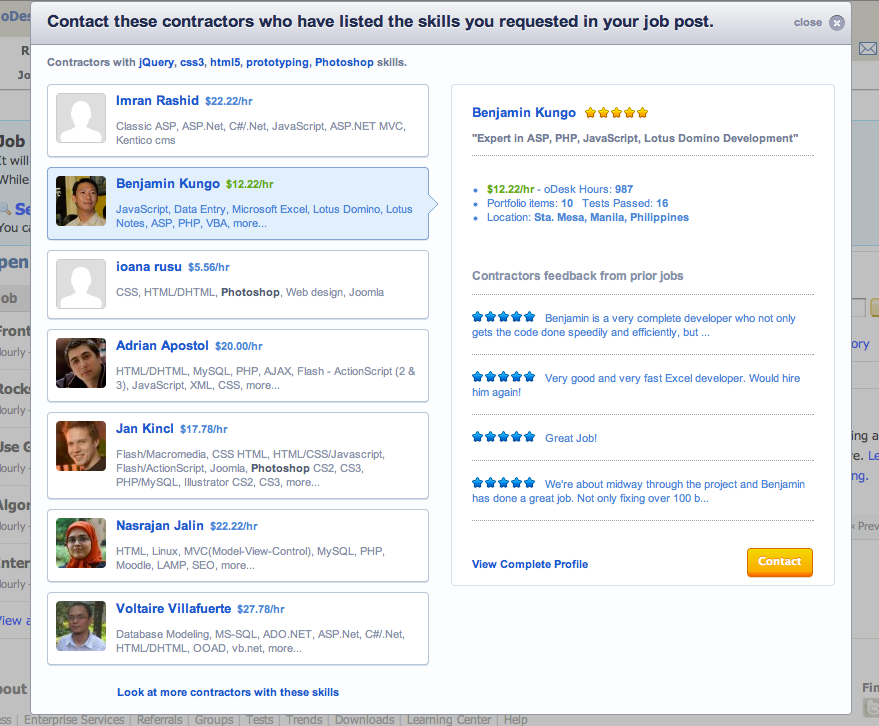
\includegraphics[width=20mm]{present_screenshot.png} \end{figure}
\end{minipage}
}

\vspace{\textheight}

\end{minipage}
}
\end{animateinline}
\end{frame}

\begin{frame}{}
\begin{animateinline}[autoplay]{10}
\multiframe{5}{i=0+25}{
\begin{minipage}{\textwidth}
\begin{center}
\vspace{1mm}

\textcolor{gray\i}{Overview of oDesk}

\textcolor{gray\i}{Marketplace}

\vspace{1mm}
\end{center}
\end{minipage}
}
\end{animateinline}
\end{frame}

\begin{frame}{}
\begin{animateinline}[autoplay]{10}
\multiframe{5}{i=0+25}{
\begin{minipage}{\textwidth}
\begin{center}
\vspace{1mm}

\textcolor{gray\i}{Preference for}

\textcolor{gray\i}{Recruited Candidates}

\vspace{1mm}
\end{center}
\end{minipage}
}
\end{animateinline}
\end{frame}

\begin{frame}{}
\begin{animateinline}[autoplay]{10}
\multiframe{9}{ii=0+25}{
\pgfmathtruncatemacro{\ifirst}{min(100,max(0,\ii))}%
\pgfmathtruncatemacro{\isecond}{min(100,max(0,\ii - 100))}%
\begin{minipage}{\textwidth}
\begin{center}
\vspace{1mm}

\textcolor{gray\ifirst}{The Experiment:}

\textcolor{gray\isecond}{Algorithmic Candidate}

\textcolor{gray\isecond}{Recommendations}

\vspace{1mm}
\end{center}
\end{minipage}
}
\end{animateinline}
\end{frame}

\begin{frame}
\begin{animateinline}[autoplay]{10}
\multiframe{25}{ii=0+25}{
\begin{minipage}{\textwidth}
\pgfmathtruncatemacro{\ifirst}{min(100,max(0,\ii))}%
\pgfmathtruncatemacro{\isecond}{min(100,max(0,\ii - 100))}%
\pgfmathtruncatemacro{\ithird}{min(100,max(0,\ii - 200))}%
\pgfmathtruncatemacro{\ifourth}{min(100,max(0,\ii - 300))}%
\pgfmathtruncatemacro{\ififth}{min(100,max(0,\ii - 400))}%
\pgfmathtruncatemacro{\isixth}{min(100,max(0,\ii - 500))}%

\pgfmathsetmacro{\itrans}{\ifirst/100}%

\nointerlineskip
\putattrans{0.65}{0.5}{\itrans}{
\begin{minipage}{80mm}
\begin{figure}[H] \centering 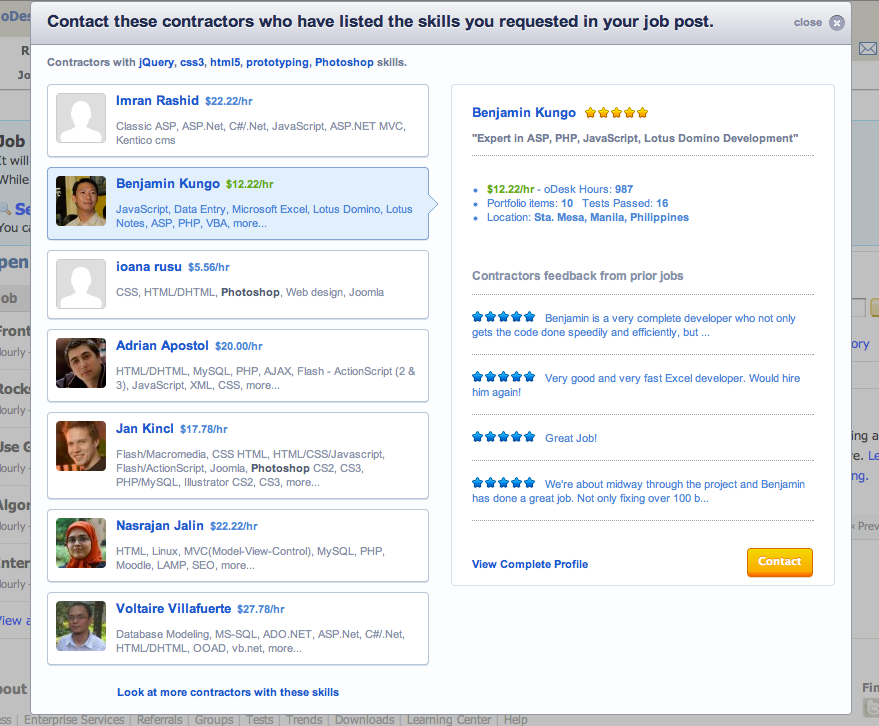
\includegraphics[width=80mm]{present_screenshot.png} \end{figure}
\end{minipage}
}

\nointerlineskip
\putat{0.14}{0.15}{
\normalsize
\textcolor{gray\isecond}{Required skills}
}

\nointerlineskip
\putat{0.14}{0.3}{
\normalsize
\textcolor{gray\ithird}{Contractor skills}
}

\nointerlineskip
\putat{0.14}{0.45}{
\normalsize
\textcolor{gray\ifourth}{Hourly rate}
}

\nointerlineskip
\putat{0.14}{0.56}{
\normalsize
\textcolor{gray\ififth}{Testing info,}
}

\nointerlineskip
\putat{0.14}{0.62}{
\normalsize
\textcolor{gray\ififth}{location,}
}

\nointerlineskip
\putat{0.14}{0.68}{
\normalsize
\textcolor{gray\ififth}{on-platform}
}

\nointerlineskip
\putat{0.14}{0.74}{
\normalsize
\textcolor{gray\ififth}{experience}
}

\nointerlineskip
\putat{0.14}{0.85}{
\normalsize
\textcolor{gray\isixth}{Feedback}
}

\pgfmathsetmacro{\arrxsecond}{83+(37*(\isecond/100))}%
\pgfmathsetmacro{\arrysecond}{-35-(5*(\isecond/100))}%
\pgfmathsetmacro{\arrxthird}{70+(45*(\ithird/100))}%
\pgfmathsetmacro{\arrythird}{-78-(2*(\ithird/100))}%
\pgfmathsetmacro{\arrxfourth}{75+(58*(\ifourth/100))}%
\pgfmathsetmacro{\arryfourth}{-105+(12*(\ifourth/100))}%
\pgfmathsetmacro{\arrxfifth}{70+(135*(\ififth/100))}%
\pgfmathsetmacro{\arryfifth}{-145+(65*(\ififth/100))}%
\pgfmathsetmacro{\arrxsixth}{70+(135*(\isixth/100))}%
\pgfmathsetmacro{\arrysixth}{-200+(80*(\isixth/100))}%

\nointerlineskip
\begin{tikzpicture}[overlay]
\ifthenelse{\isecond > 0}
{\draw[->,line width=2pt] (83pt,-35pt) -- (\arrxsecond pt,\arrysecond pt);}
{}
\ifthenelse{\ithird > 0}
{\draw[->,line width=2pt] (70pt,-78pt) -- (\arrxthird pt,\arrythird pt);}
{}
\ifthenelse{\ifourth > 0}
{\draw[->,line width=2pt] (75pt,-105pt) -- (\arrxfourth pt,\arryfourth pt);}
{}
\ifthenelse{\ififth > 0}
{\draw[->,line width=2pt] (70pt,-145pt) -- (\arrxfifth pt,\arryfifth pt);}
{}
\ifthenelse{\isixth > 0}
{\draw[->,line width=2pt] (70pt,-200pt) -- (\arrxsixth pt,\arrysixth pt);}
{}
\end{tikzpicture}

\vspace{\textheight}

\end{minipage}
}
\end{animateinline}
\end{frame}

\begin{frame}{}
\begin{animateinline}[autoplay]{10}
\multiframe{5}{i=0+25}{
\begin{minipage}{\textwidth}
\begin{center}
\vspace{1mm}

\textcolor{gray\i}{A model of employer}

\textcolor{gray\i}{search and screening}

\vspace{1mm}
\end{center}
\end{minipage}
}
\end{animateinline}
\end{frame}

\begin{frame}
\begin{animateinline}[autoplay]{10}
\multiframe{21}{ii=0+25}{
\begin{minipage}{\textwidth}
\pgfmathtruncatemacro{\ifirst}{min(100,max(0,\ii))}%
\pgfmathtruncatemacro{\isecond}{min(100,max(0,\ii - 100))}%
\pgfmathtruncatemacro{\ithird}{min(100,max(0,\ii - 200))}%
\pgfmathtruncatemacro{\ifourth}{min(100,max(0,\ii - 300))}%
\pgfmathtruncatemacro{\ififth}{min(100,max(0,\ii - 400))}%

\pgfmathsetmacro{\itrans}{\ifirst/100}%

\nointerlineskip
\putattrans{0.5}{0.59}{\itrans}{
\begin{minipage}{80mm}
\begin{figure}[H] \centering 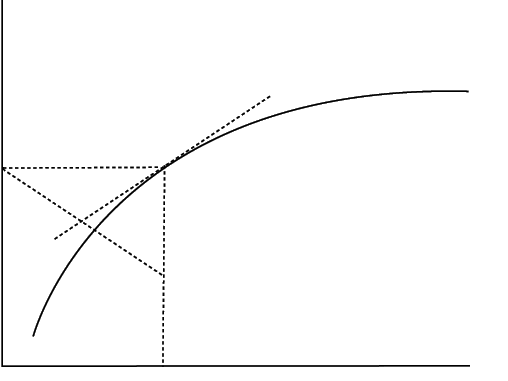
\includegraphics[width=80mm]{present_dia1.png} \end{figure}
\end{minipage}
}

\nointerlineskip
\putat{0.14}{0.2}{
\normalsize
\textcolor{gray\isecond}{Expected benefit}
}

\nointerlineskip
\putat{0.7}{0.29}{
\normalsize
\textcolor{gray\ithird}{Firm picks a* such}
}

\nointerlineskip
\putat{0.7}{0.35}{
\normalsize
\textcolor{gray\ithird}{that marginal benefit = marginal cost}
}

\nointerlineskip
\putat{0.7}{0.65}{
\normalsize
\textcolor{gray\ifourth}{Screening}
}

\nointerlineskip
\putat{0.7}{0.71}{
\normalsize
\textcolor{gray\ifourth}{costs are ca*}
}

\nointerlineskip
\putat{0.9}{0.9}{
\normalsize
\textcolor{gray\ififth}{\# apps}
}

\nointerlineskip
\putat{0.9}{0.96}{
\normalsize
\textcolor{gray\ififth}{screened}
}

\vspace{\textheight}

\end{minipage}
}
\end{animateinline}
\end{frame}

\begin{frame}
\begin{animateinline}[autoplay]{10}
\multiframe{25}{ii=0+25}{
\begin{minipage}{\textwidth}
\pgfmathtruncatemacro{\ifirst}{min(100,max(0,\ii))}%
\pgfmathtruncatemacro{\isecond}{min(100,max(0,\ii - 100))}%
\pgfmathtruncatemacro{\ithird}{min(100,max(0,\ii - 200))}%
\pgfmathtruncatemacro{\ifourth}{min(100,max(0,\ii - 300))}%
\pgfmathtruncatemacro{\ififth}{min(100,max(0,\ii - 400))}%
\pgfmathtruncatemacro{\isixth}{min(100,max(0,\ii - 500))}%
\begin{center}
\textcolor{gray\ifirst}{Model}
\end{center}

\begin{itemize}
\large
\variitem{gray\isecond} \textcolor{gray\isecond}{Employer posts a vacancy and gets $ A $ applicants}
\begin{itemize}
\large
\variitem{gray\ithird} \textcolor{gray\ithird}{Applicants have some probability $ q_i \sim F $ of being a match}

\variitem{gray\ifourth} \textcolor{gray\ifourth}{Employers rank applicants by $ q $ and take the top $ a $ applicants to screen 
(which reveals whether or not a match but costs $ c $)}

\variitem{gray\ififth} \textcolor{gray\ififth}{Firm needs only one match; gets value $ v $}
\end{itemize}

\variitem{gray\isixth} \textcolor{gray\isixth}{Process generates a \emph{hiring function} $ h(a; A) $}
\end{itemize}

\end{minipage}
}
\end{animateinline}
\end{frame}

\begin{frame}
\begin{animateinline}[autoplay]{10}
\multiframe{13}{ii=0+25}{
\begin{minipage}{\textwidth}
\pgfmathtruncatemacro{\ifirst}{min(100,max(0,\ii))}%
\pgfmathtruncatemacro{\isecond}{min(100,max(0,\ii - 100))}%
\pgfmathtruncatemacro{\ithird}{min(100,max(0,\ii - 200))}%
\begin{center}
\textcolor{gray\ifirst}{Recruiting}
\end{center}

\begin{itemize}
\Large
\variitem{gray\isecond} \textcolor{gray\isecond}{As a cost $ s $, firms can recruit}

\variitem{gray\ithird} \textcolor{gray\ithird}{Recruiting increases the quantity of 
applicants and average quality of applicants}
\end{itemize}

\end{minipage}
}
\end{animateinline}
\end{frame}

\begin{frame}{}
\begin{animateinline}[autoplay]{10}
\begin{minipage}{\textwidth}
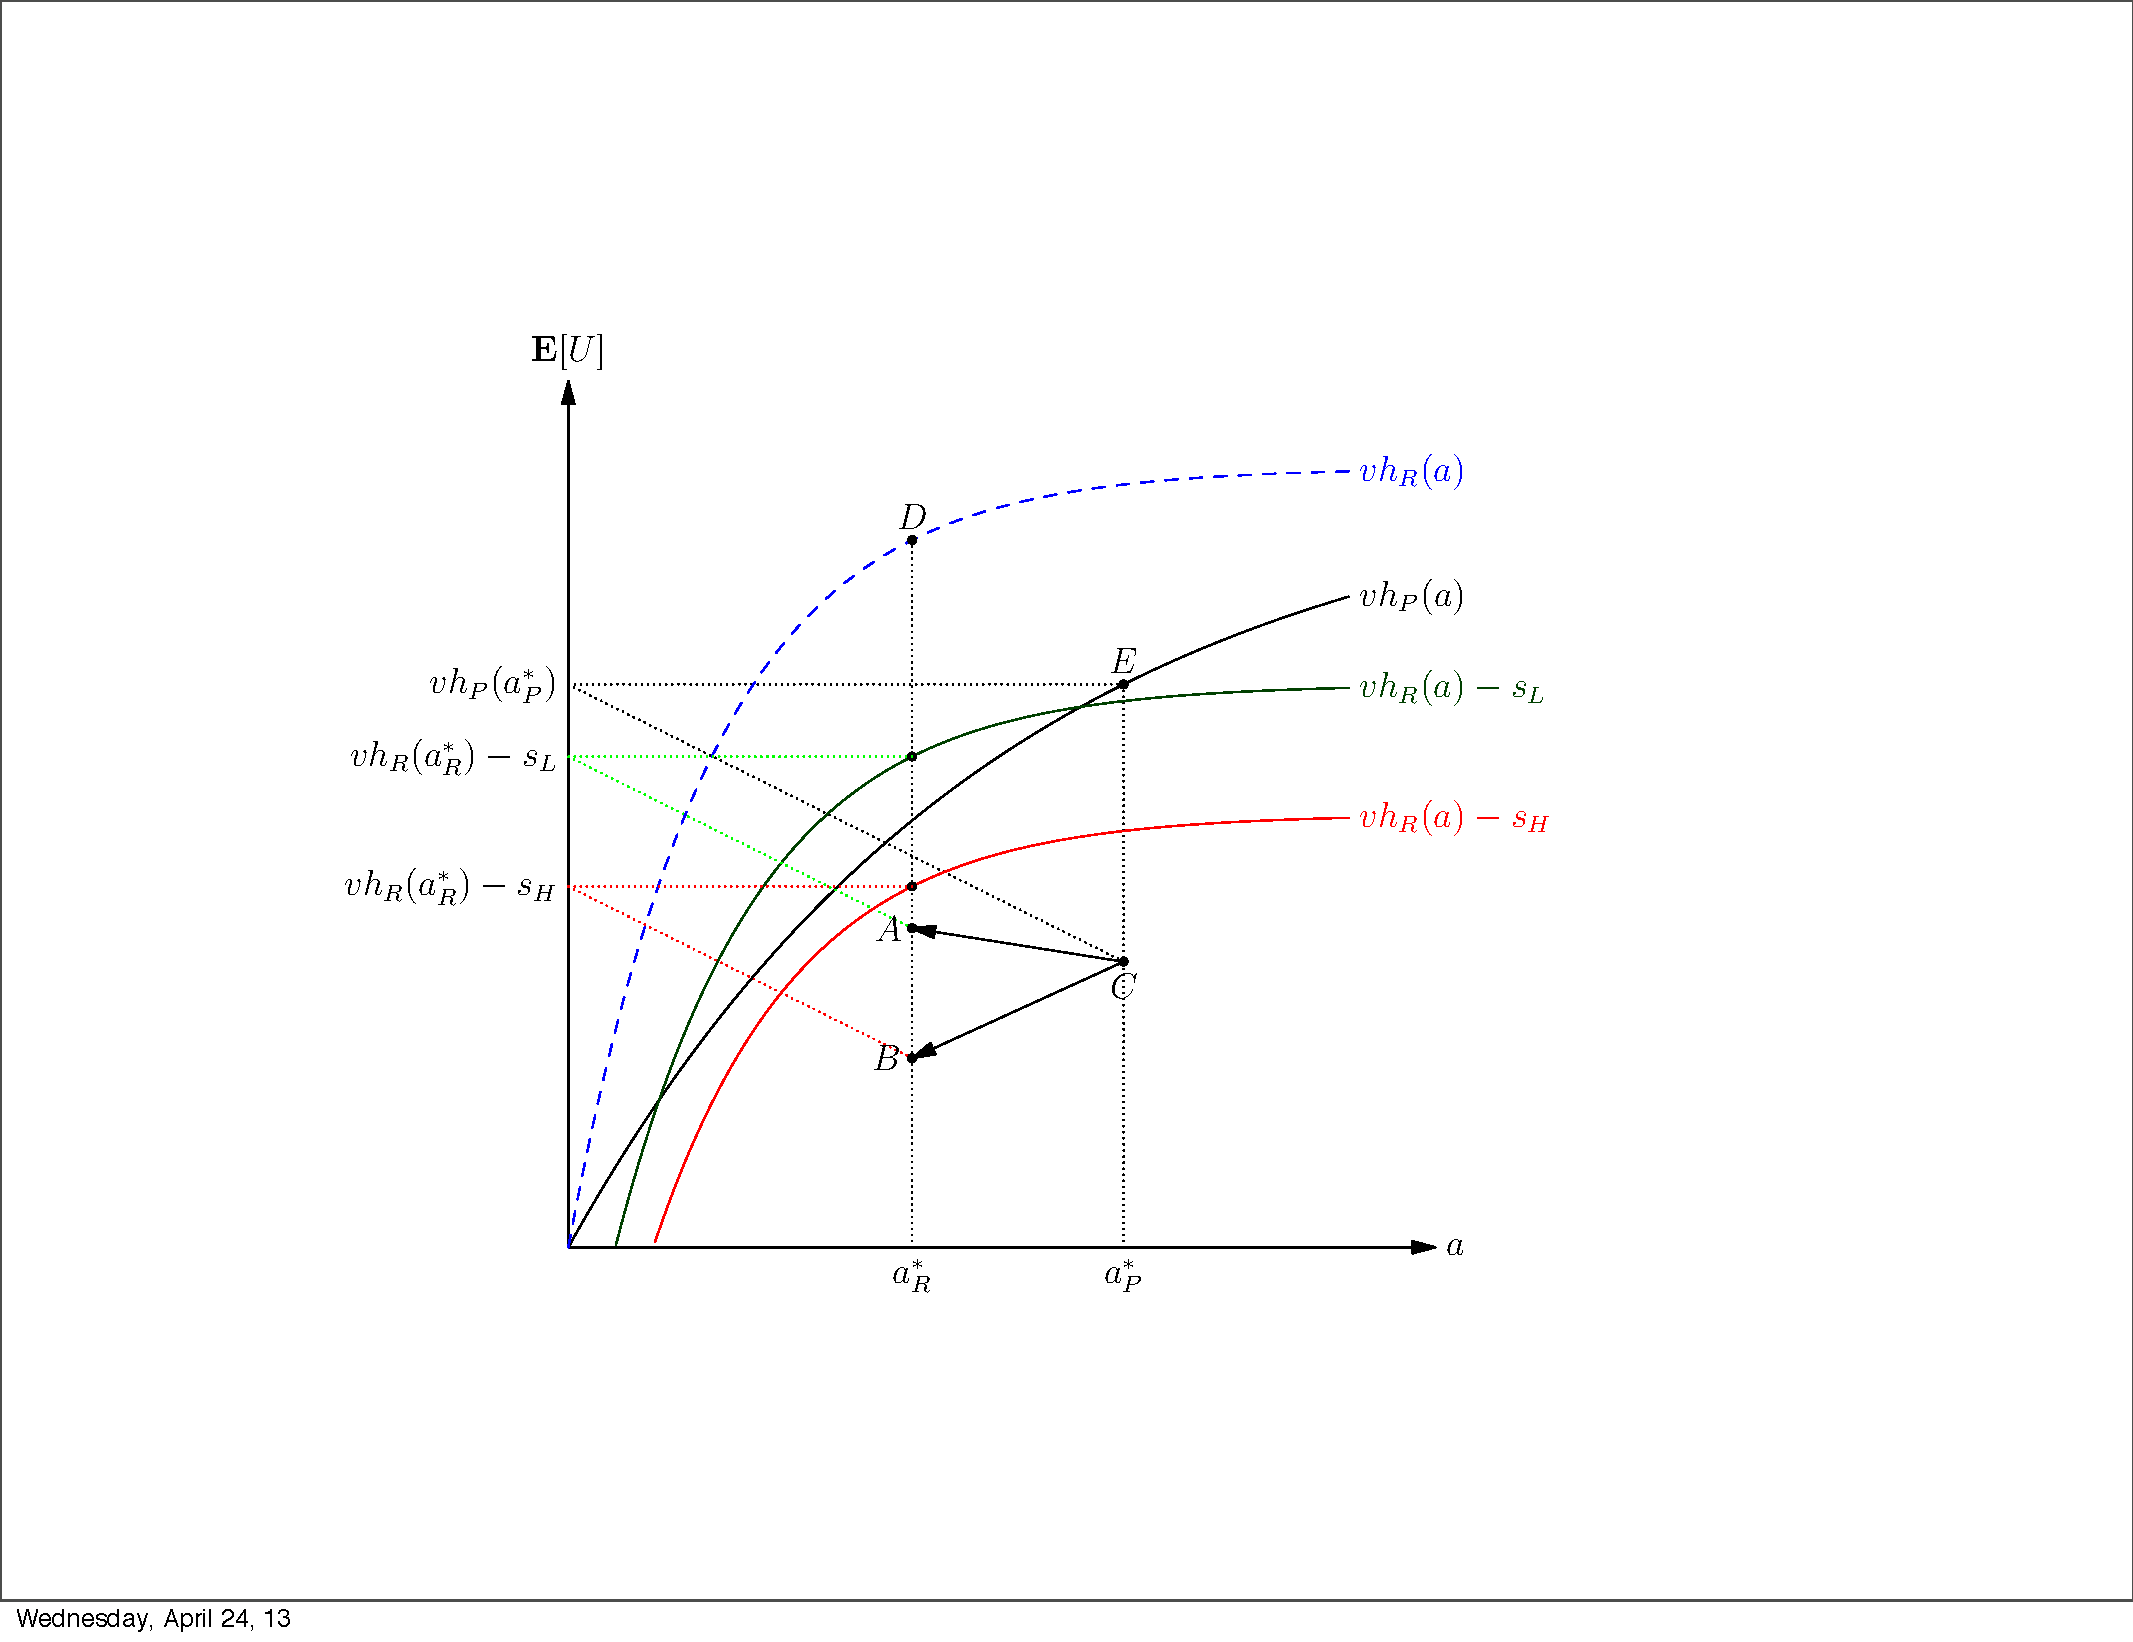
\includegraphics[trim=5cm 5.8cm 3cm 5cm,clip=true,width=140mm]{present_pdf1.pdf}

\vspace{\textheight}

\end{minipage}
\end{animateinline}
\end{frame}

\begin{frame}{}
\begin{animateinline}[autoplay]{10}
\multiframe{5}{i=0+25}{
\begin{minipage}{\textwidth}
\begin{center}
\vspace{1mm}

\textcolor{gray\i}{Experimental results}

\vspace{1mm}
\end{center}
\end{minipage}
}
\end{animateinline}
\end{frame}

\begin{frame}
\begin{animateinline}[autoplay]{10}
\multiframe{5}{ii=0+25}{
\begin{minipage}{\textwidth}
\pgfmathtruncatemacro{\ifirst}{min(100,max(0,\ii))}%

\pgfmathsetmacro{\itrans}{\ifirst/100}%

\nointerlineskip
\putattrans{0.5}{0.5}{\itrans}{
\begin{minipage}{\textwidth}
\begin{figure}[H] \centering 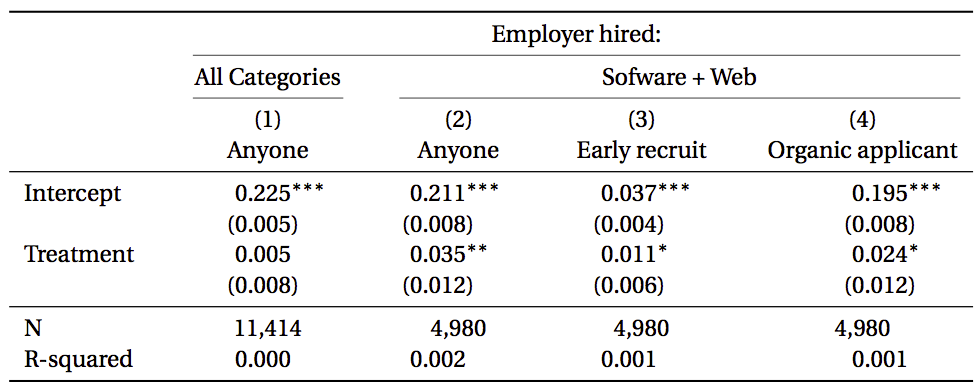
\includegraphics[width=\textwidth]{present_dia2.png} \end{figure}
\end{minipage}
}

\vspace{\textheight}

\end{minipage}
}
\end{animateinline}
\end{frame}

\begin{frame}{}
\begin{animateinline}[autoplay]{10}
\begin{minipage}{\textwidth}
\vspace{1.5cm}

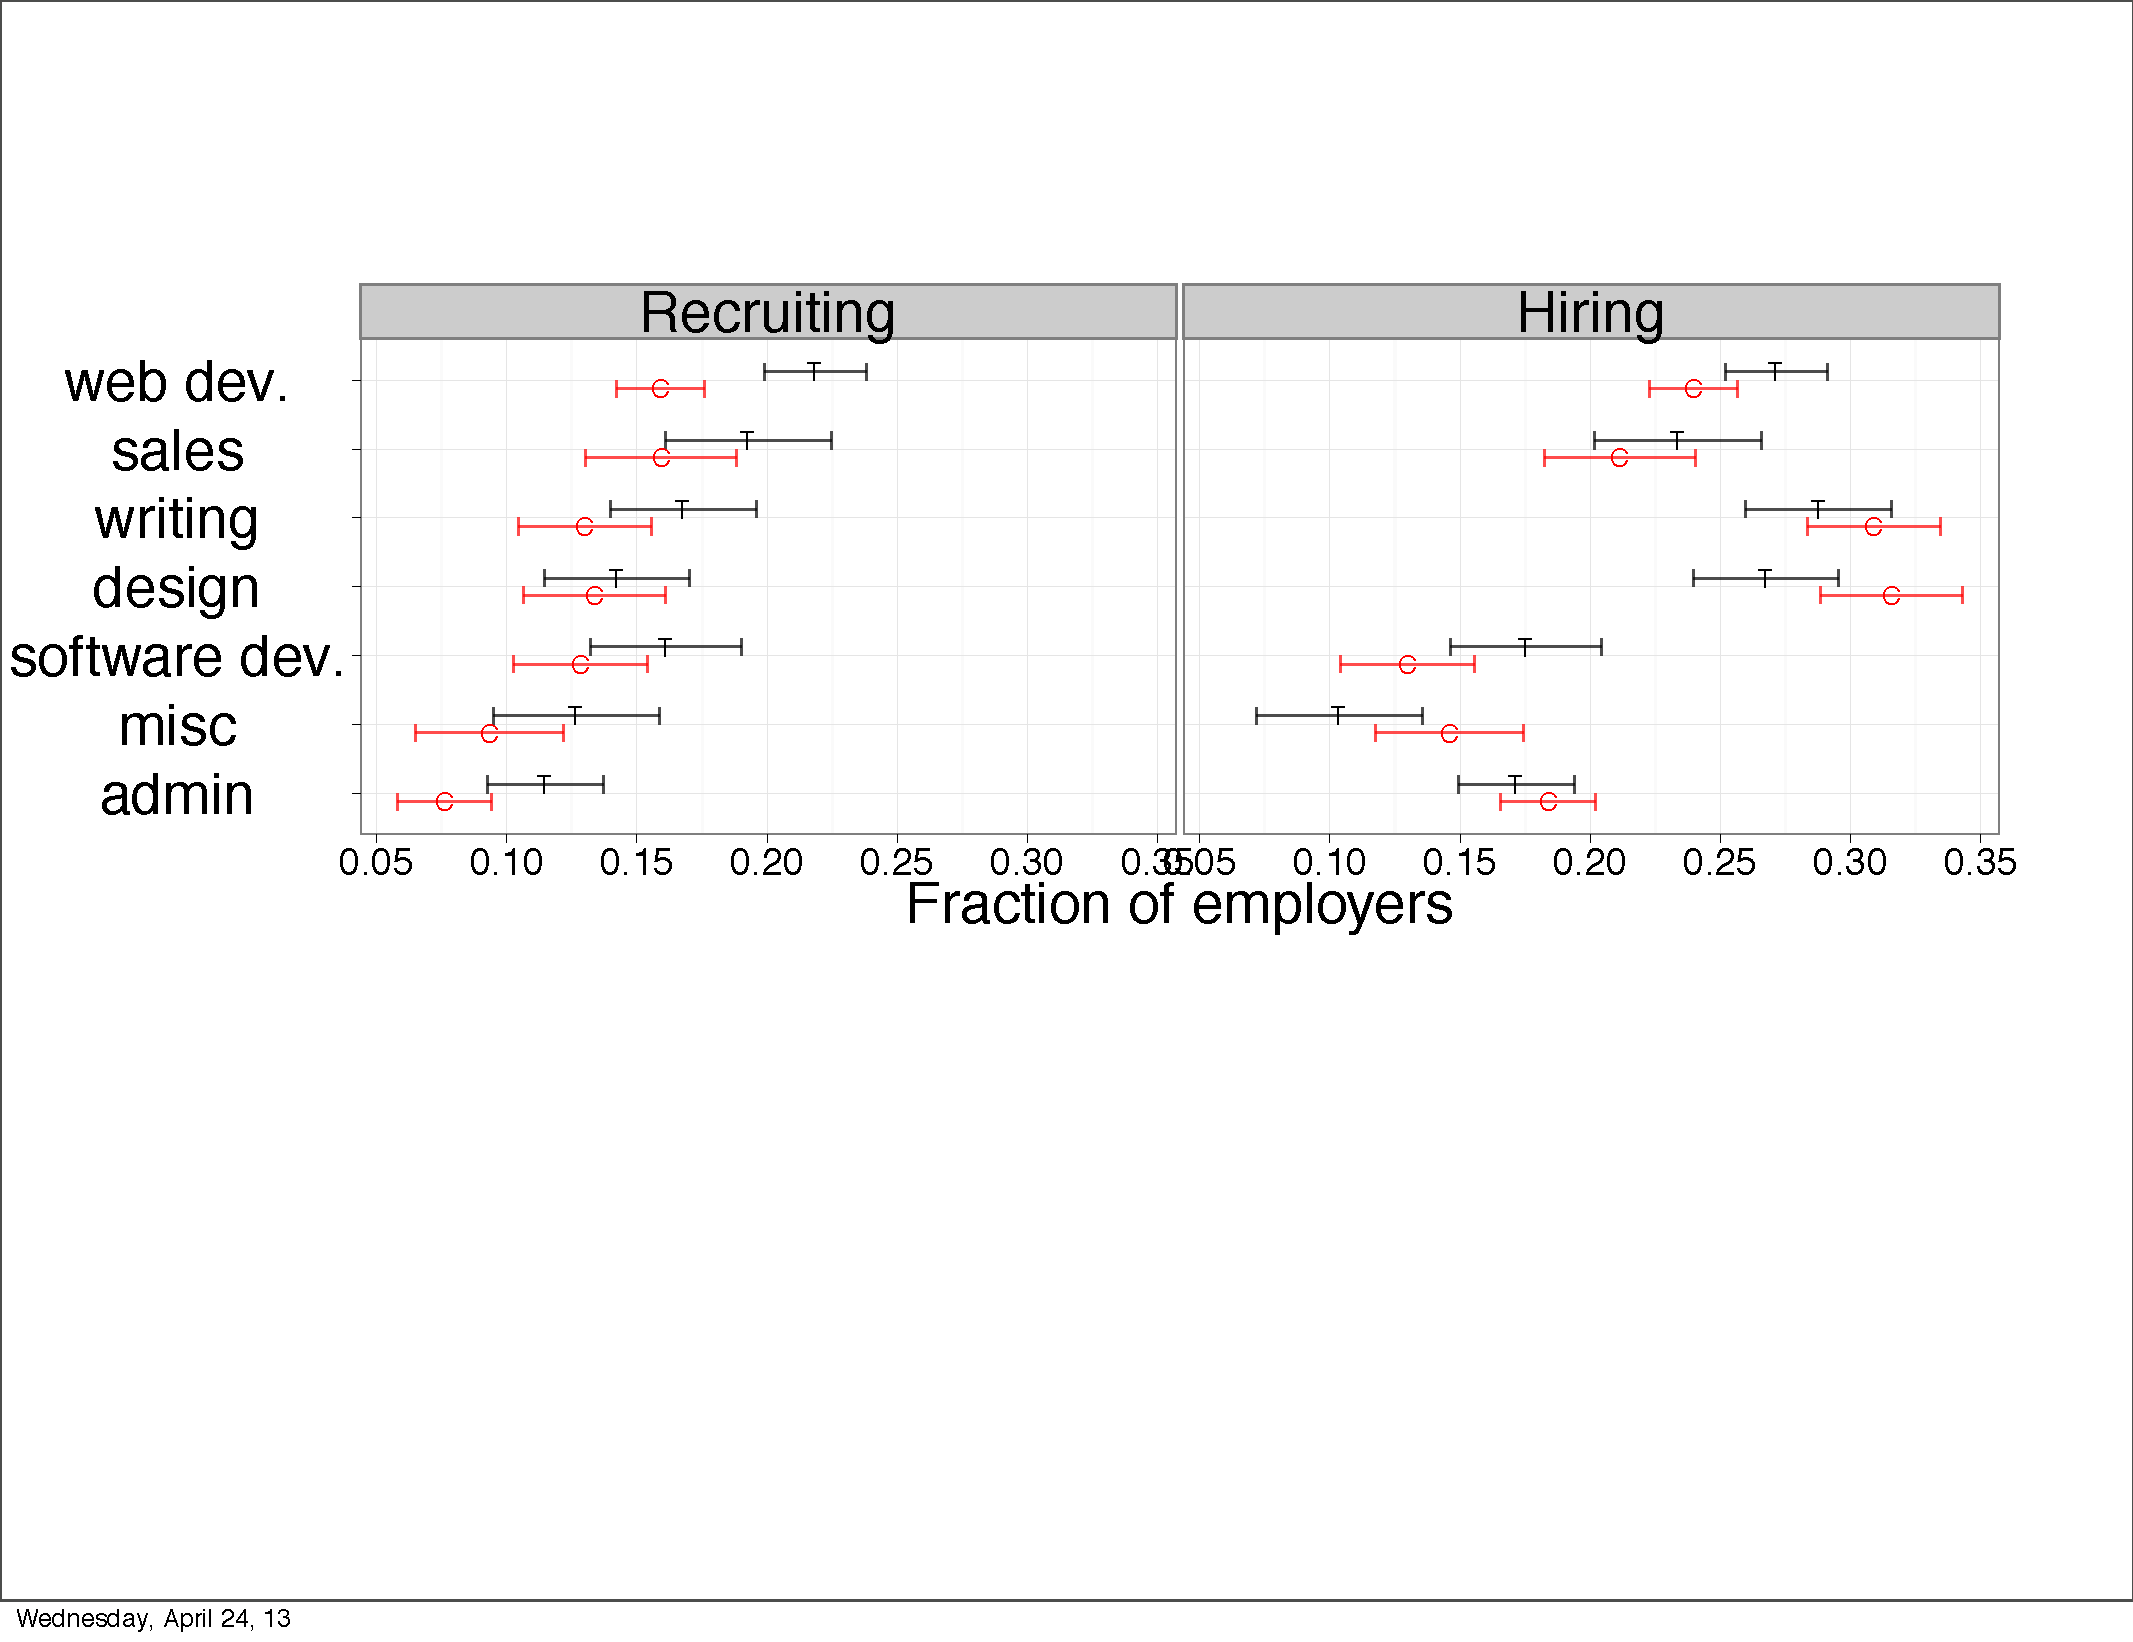
\includegraphics[trim=1mm 6cm 1mm 1mm,clip=true,width=100mm]{present_pdf2.pdf}

\vspace{\textheight}

\end{minipage}
\end{animateinline}
\end{frame}

\begin{frame}{}
\begin{animateinline}[autoplay]{10}
\multiframe{5}{i=0+25}{
\begin{minipage}{\textwidth}
\begin{center}
\vspace{1mm}

\textcolor{gray\i}{Micro-Foundations}

\textcolor{gray\i}{for Spill-Overs}

\vspace{1mm}
\end{center}
\end{minipage}
}
\end{animateinline}
\end{frame}

\begin{frame}{}
\begin{figure}[H] \centering 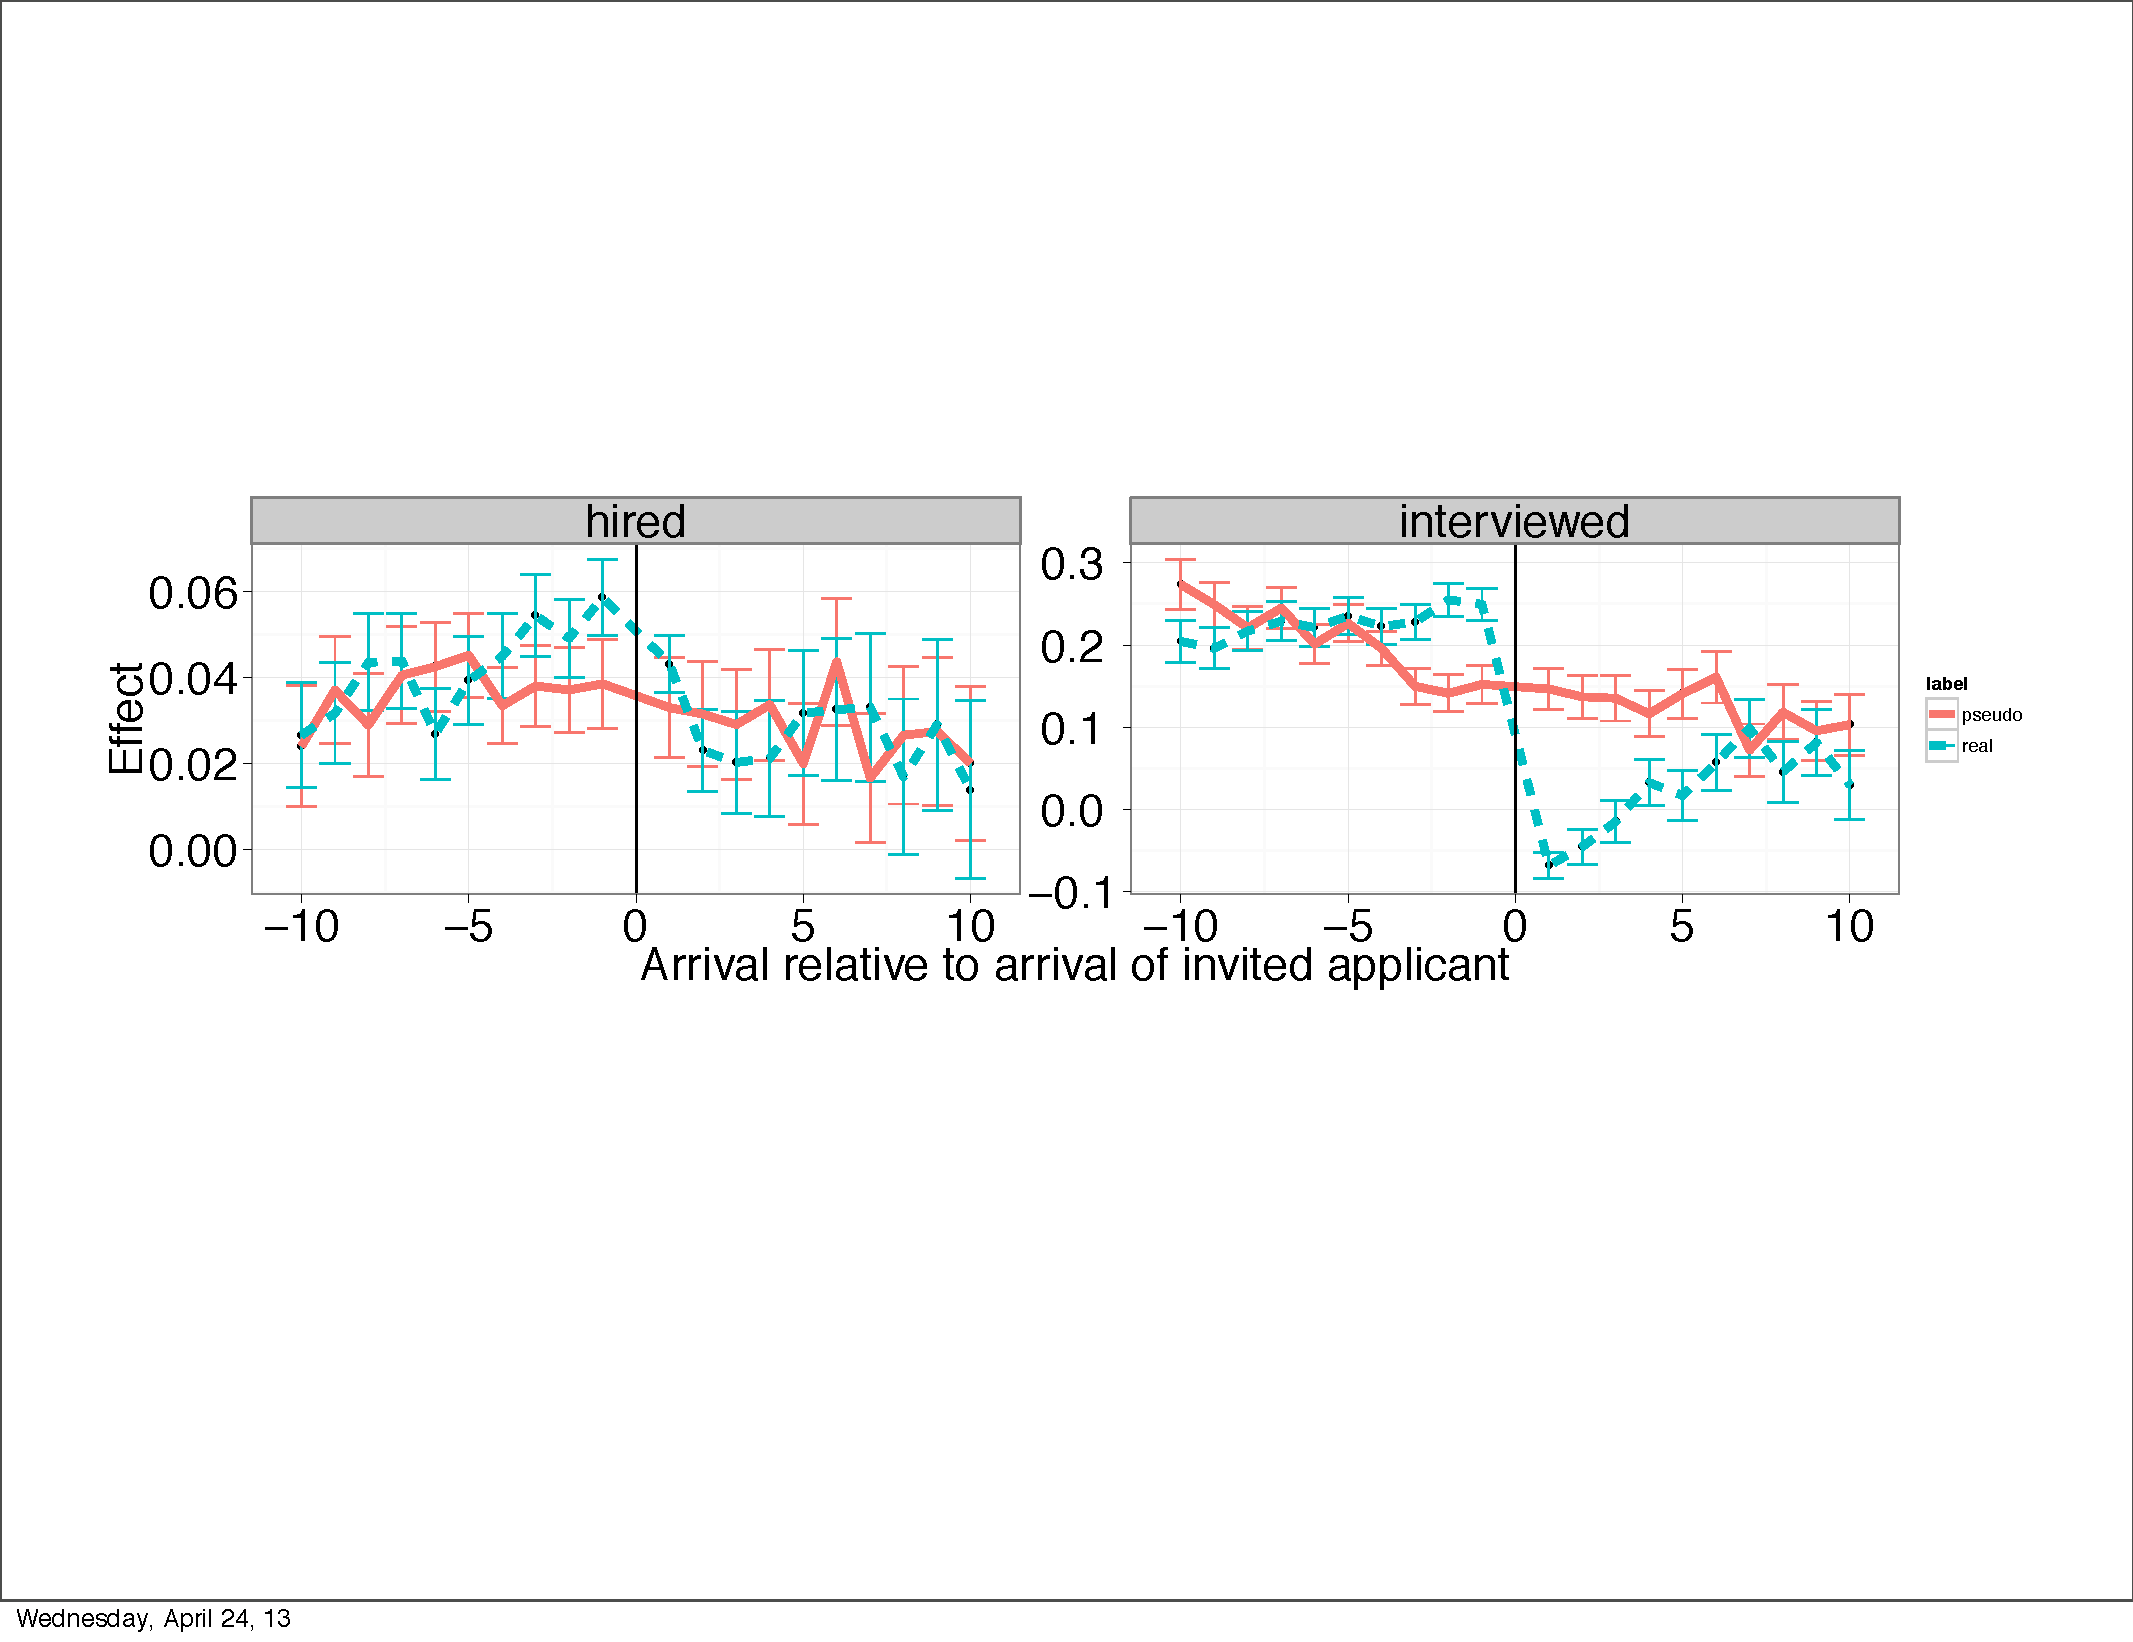
\includegraphics[trim=1.8cm 6cm 1mm 5cm,clip=true,width=120mm]{present_pdf3.pdf} \end{figure}
\end{frame}

\begin{frame}{}
\begin{animateinline}[autoplay]{10}
\multiframe{5}{i=0+25}{
\begin{minipage}{\textwidth}
\begin{center}
\vspace{1mm}

\textcolor{gray\i}{Effects of recruited}

\textcolor{gray\i}{candidates on hiring}

\vspace{1mm}
\end{center}
\end{minipage}
}
\end{animateinline}
\end{frame}

\begin{frame}{}
\begin{animateinline}[autoplay]{10}
\multiframe{5}{i=0+25}{
\begin{minipage}{\textwidth}
\begin{center}
\vspace{1mm}

\textcolor{gray\i}{Batch processing}

\vspace{1mm}
\end{center}
\end{minipage}
}
\end{animateinline}
\end{frame}

\begin{frame}{}
\begin{figure}[H] \centering 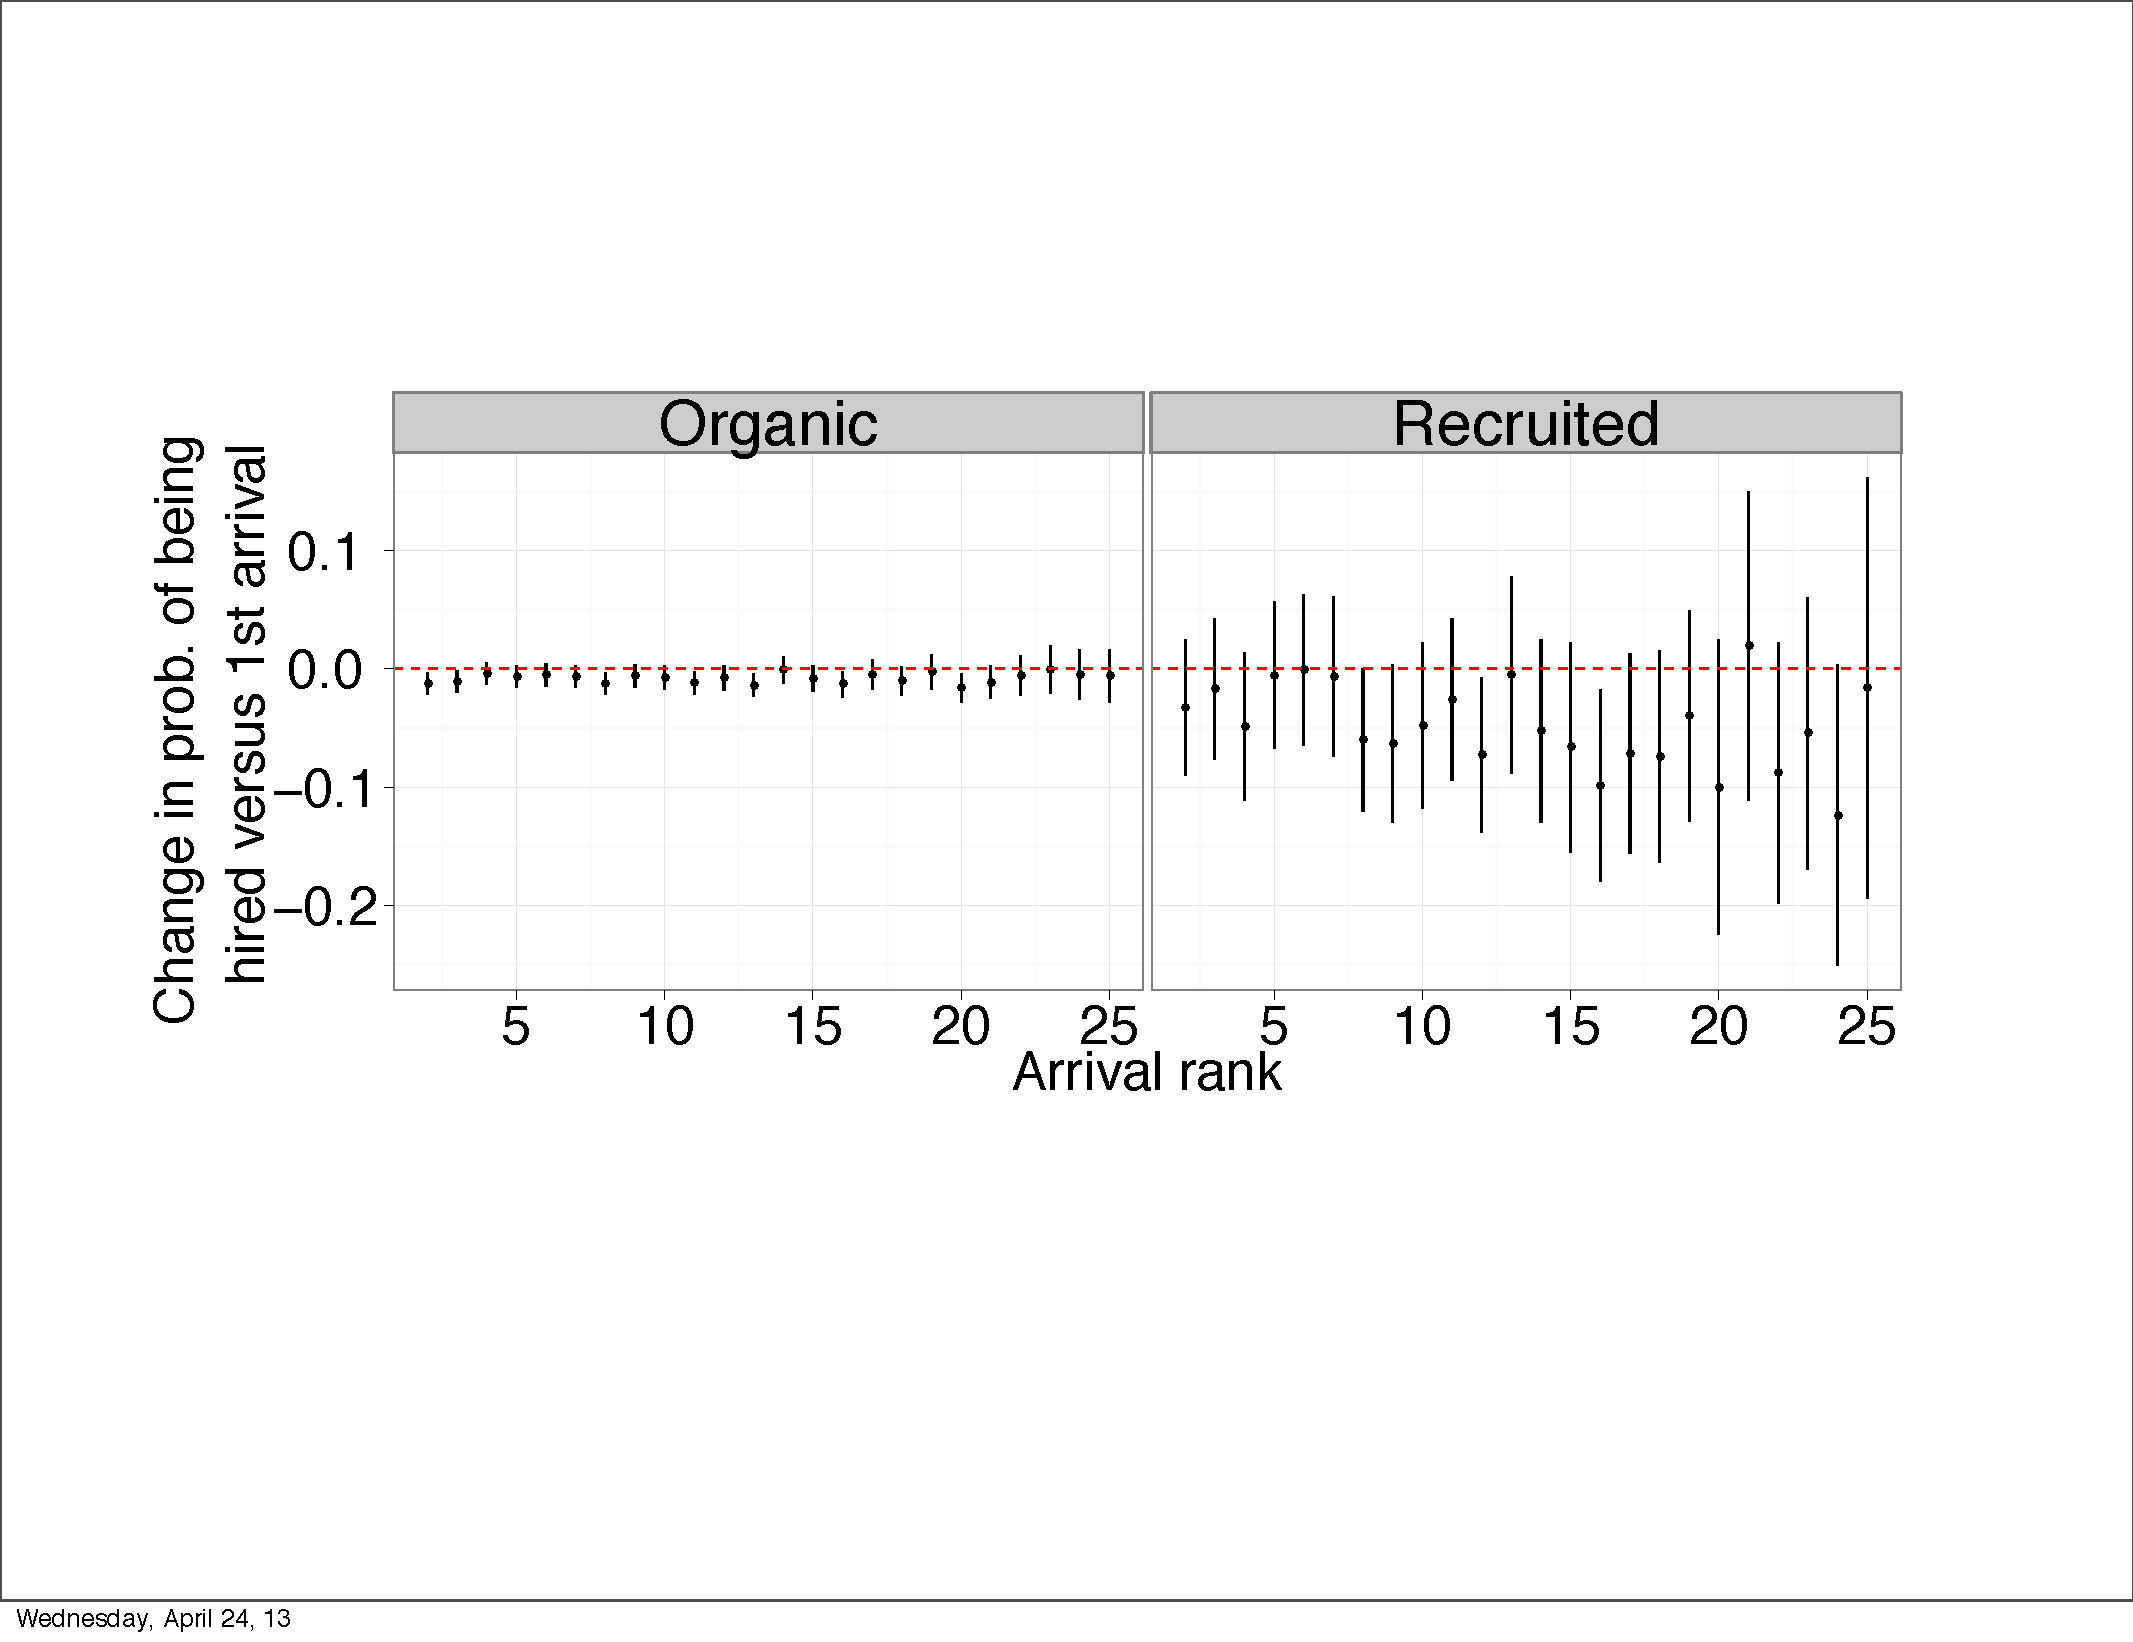
\includegraphics[trim=1.8cm 6cm 1mm 5cm,clip=true,width=120mm]{present_pdf4.pdf} \end{figure}
\end{frame}

\begin{frame}
\begin{animateinline}[autoplay]{10}
\multiframe{5}{ii=0+25}{
\begin{minipage}{\textwidth}
\pgfmathtruncatemacro{\ifirst}{min(100,max(0,\ii))}%

\pgfmathsetmacro{\itrans}{\ifirst/100}%

\nointerlineskip
\putattrans{0.5}{0.5}{\itrans}{
\begin{minipage}{\textwidth}
\begin{figure}[H] \centering 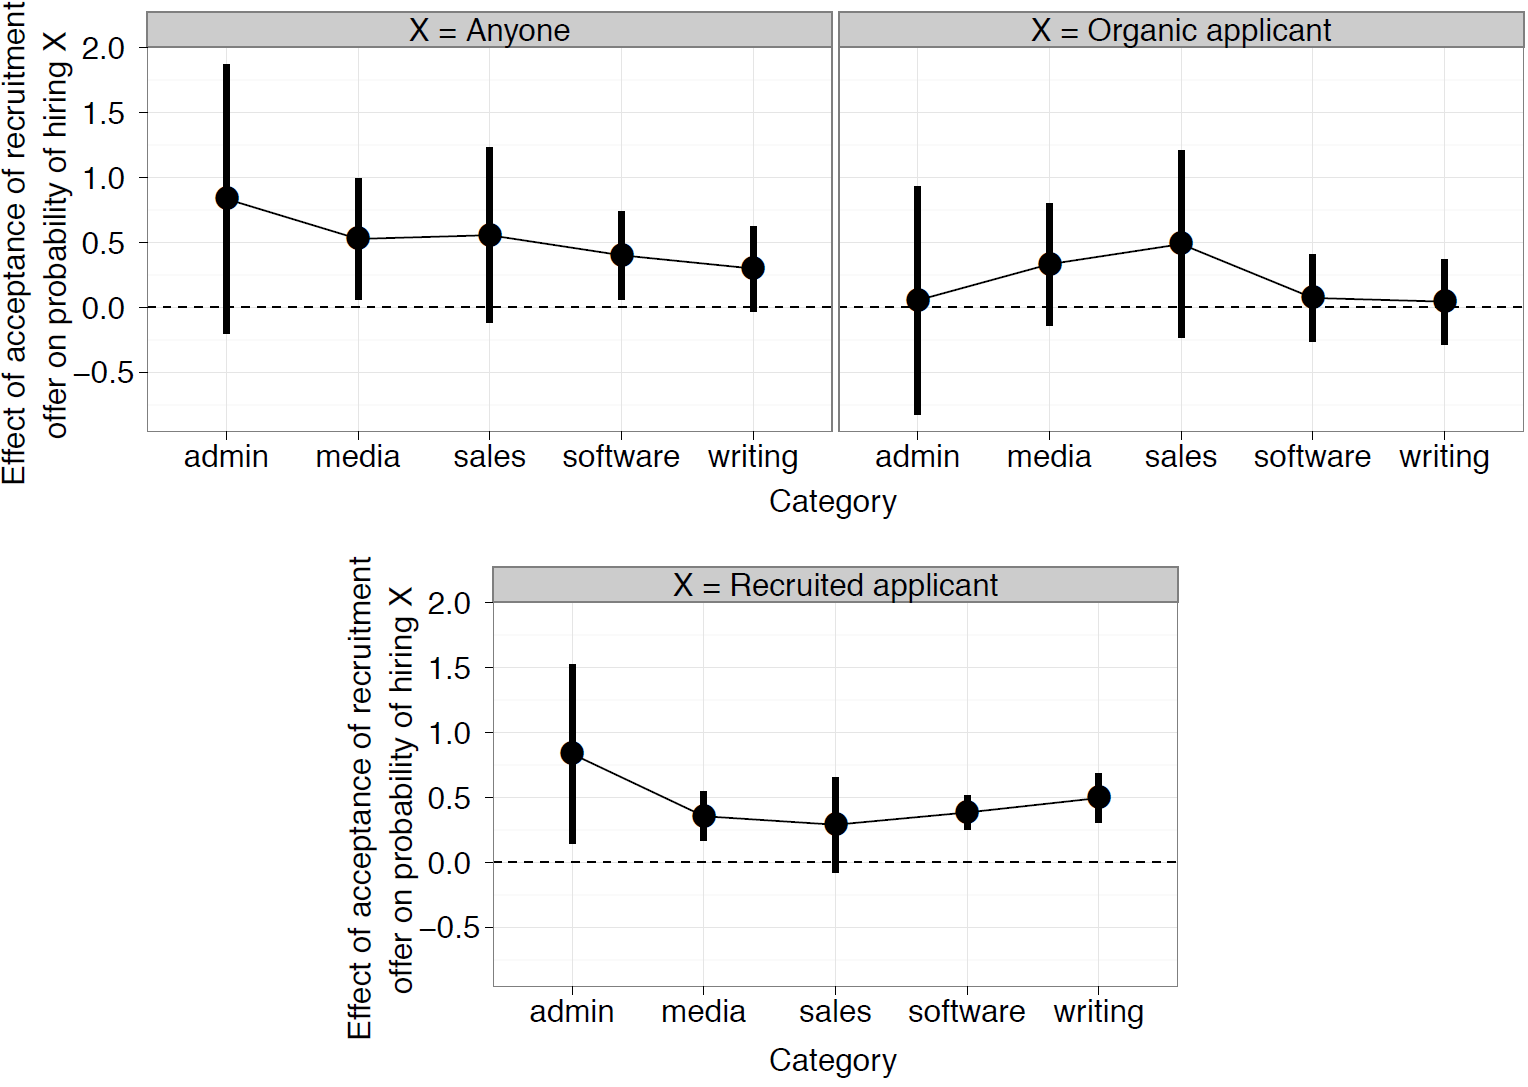
\includegraphics[width=\textwidth]{present_dia3.png} \end{figure}
\end{minipage}
}

\vspace{\textheight}

\end{minipage}
}
\end{animateinline}
\end{frame}

\begin{frame}{}
\begin{figure}[H] \centering 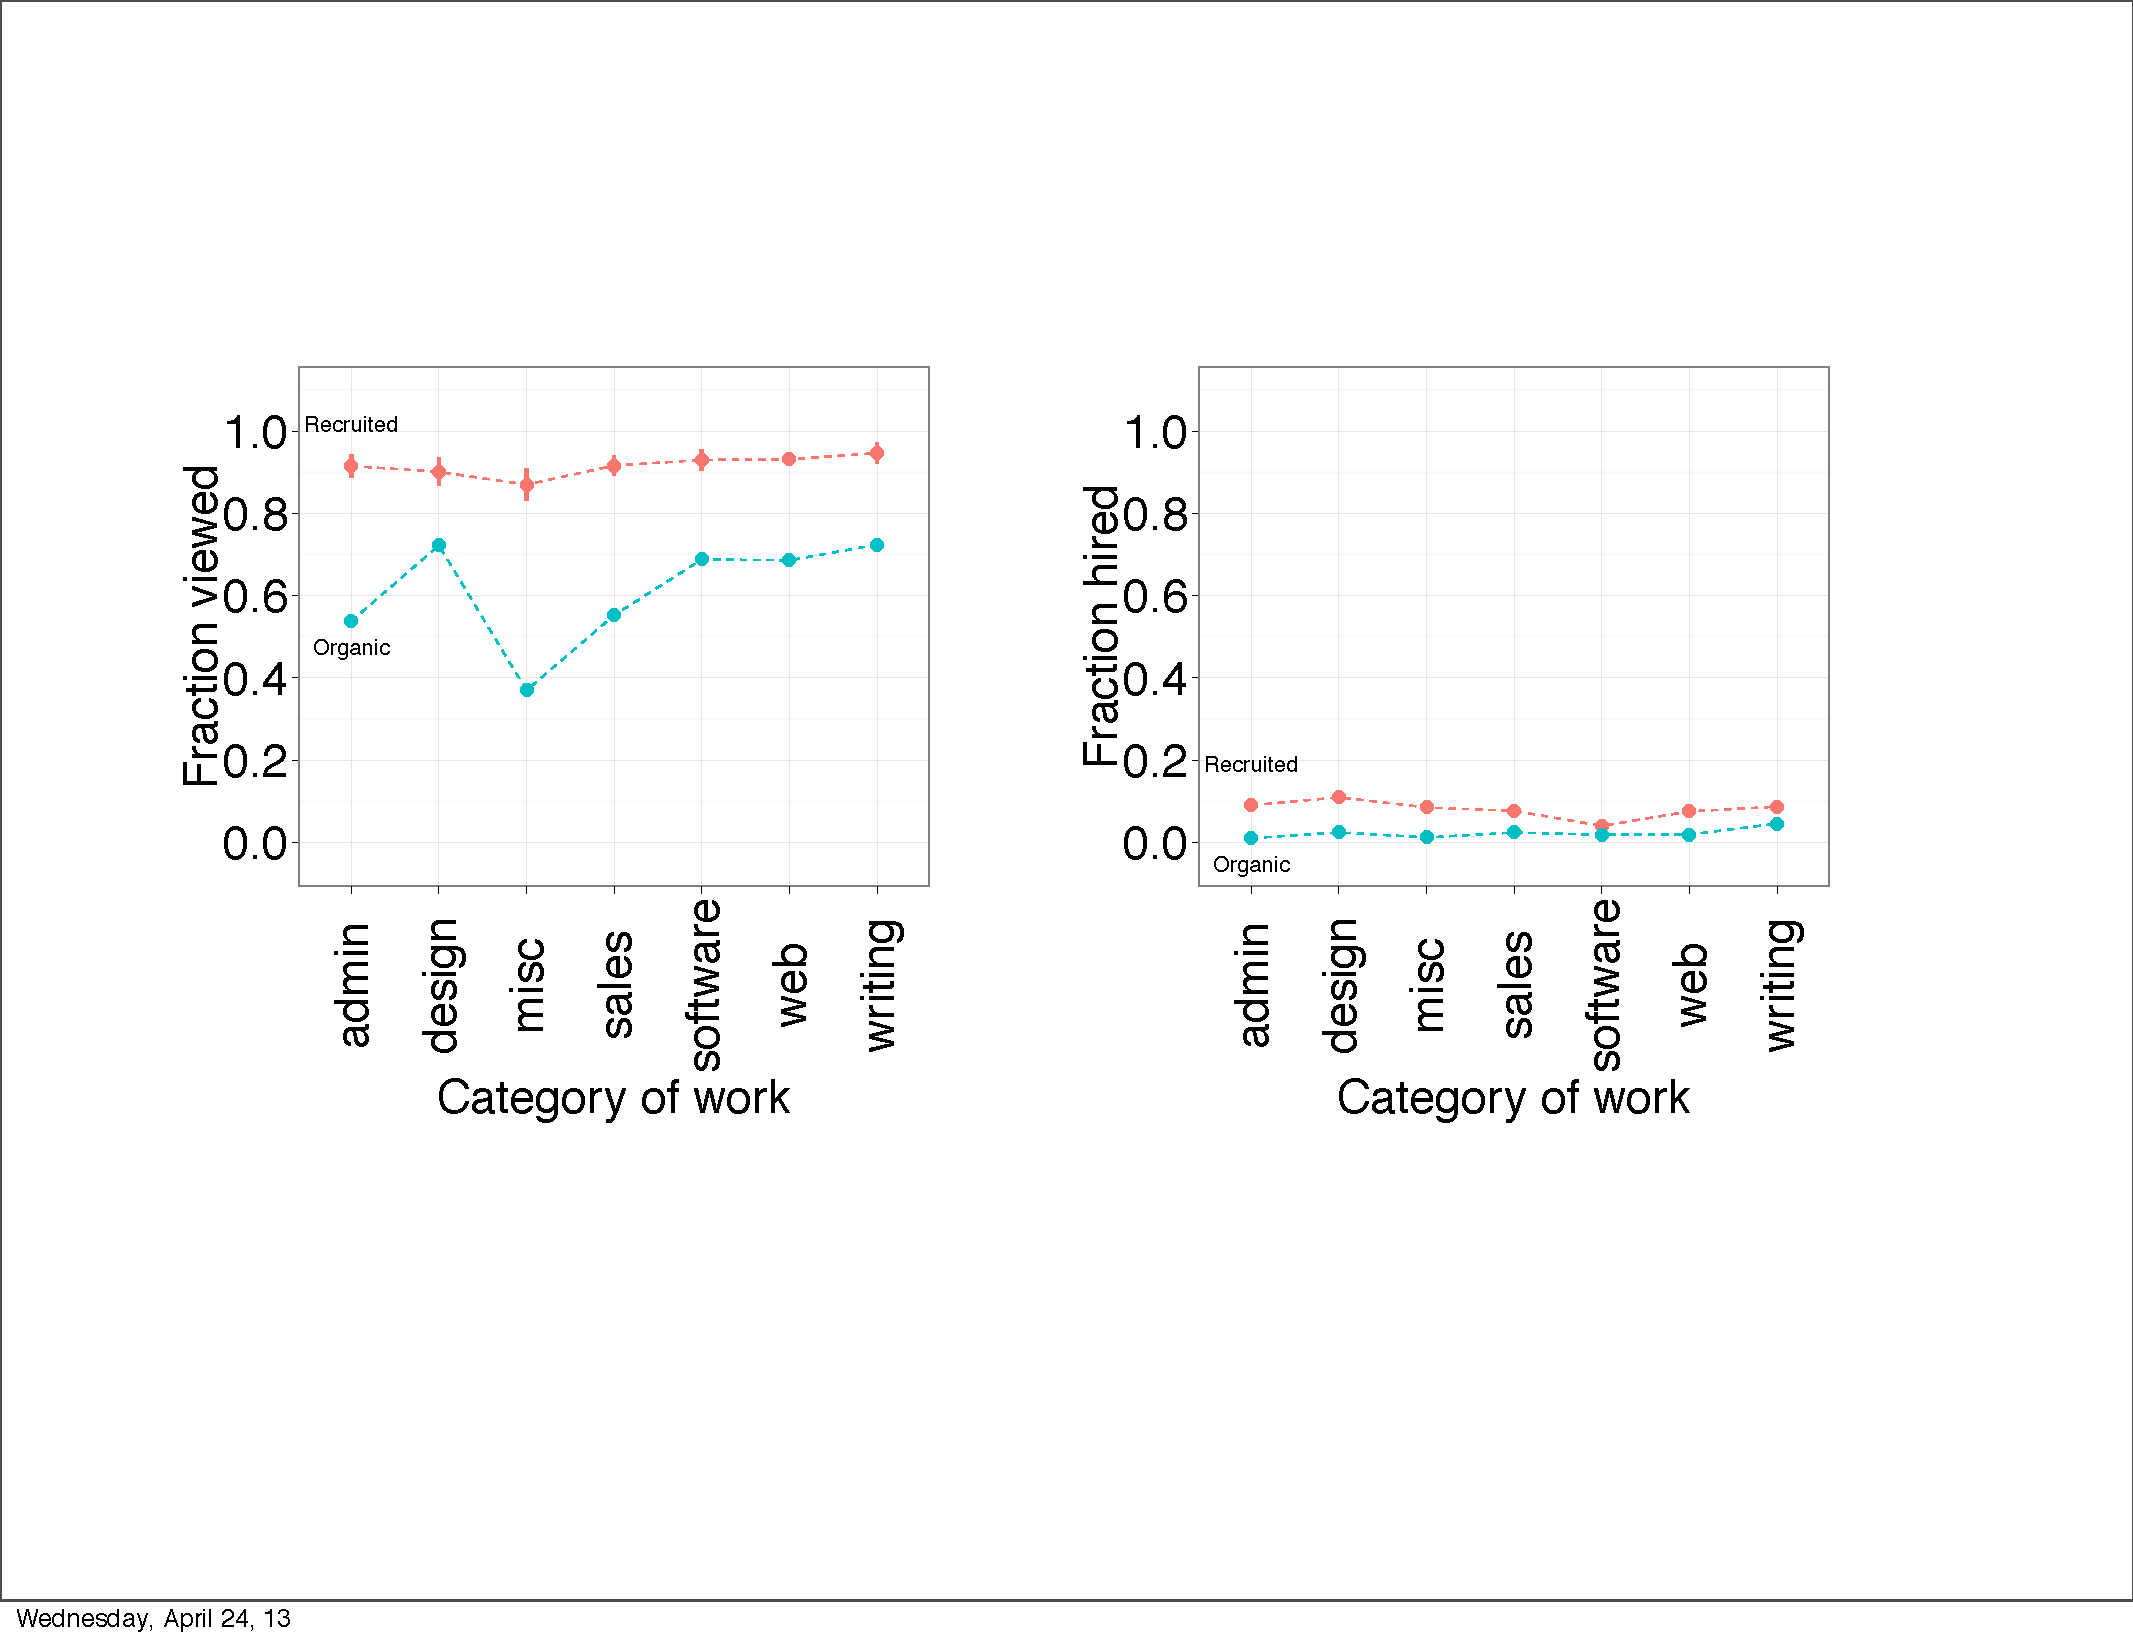
\includegraphics[trim=1.8cm 6cm 1mm 5cm,clip=true,width=120mm]{present_pdf6.pdf} \end{figure}
\end{frame}

\begin{frame}
\begin{animateinline}[autoplay]{10}
\multiframe{5}{ii=0+25}{
\begin{minipage}{\textwidth}
\pgfmathtruncatemacro{\ifirst}{min(100,max(0,\ii))}%

\pgfmathsetmacro{\itrans}{\ifirst/100}%

\nointerlineskip
\putattrans{0.5}{0.5}{\itrans}{
\begin{minipage}{\textwidth}
\begin{figure}[H] \centering 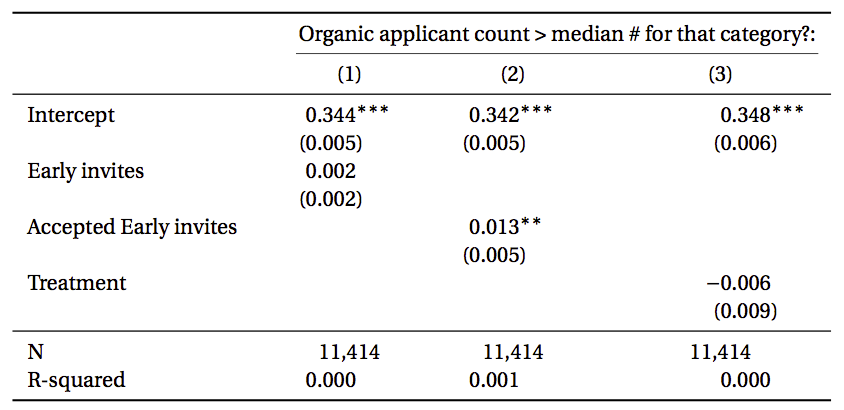
\includegraphics[width=\textwidth]{present_dia4.png} \end{figure}
\end{minipage}
}

\vspace{\textheight}

\end{minipage}
}
\end{animateinline}
\end{frame}

\begin{frame}
\begin{animateinline}[autoplay]{10}
\multiframe{25}{ii=0+25}{
\begin{minipage}{\textwidth}
\pgfmathtruncatemacro{\ifirst}{min(100,max(0,\ii))}%
\pgfmathtruncatemacro{\isecond}{min(100,max(0,\ii - 100))}%
\pgfmathtruncatemacro{\ithird}{min(100,max(0,\ii - 200))}%
\pgfmathtruncatemacro{\ifourth}{min(100,max(0,\ii - 300))}%
\pgfmathtruncatemacro{\ififth}{min(100,max(0,\ii - 400))}%
\pgfmathtruncatemacro{\isixth}{min(100,max(0,\ii - 500))}%

\pgfmathsetmacro{\itrans}{\ifirst/100}%

\nointerlineskip
\putattrans{0.45}{0.5}{\itrans}{
\begin{minipage}{0.9\textwidth}
\begin{figure}[H] \centering 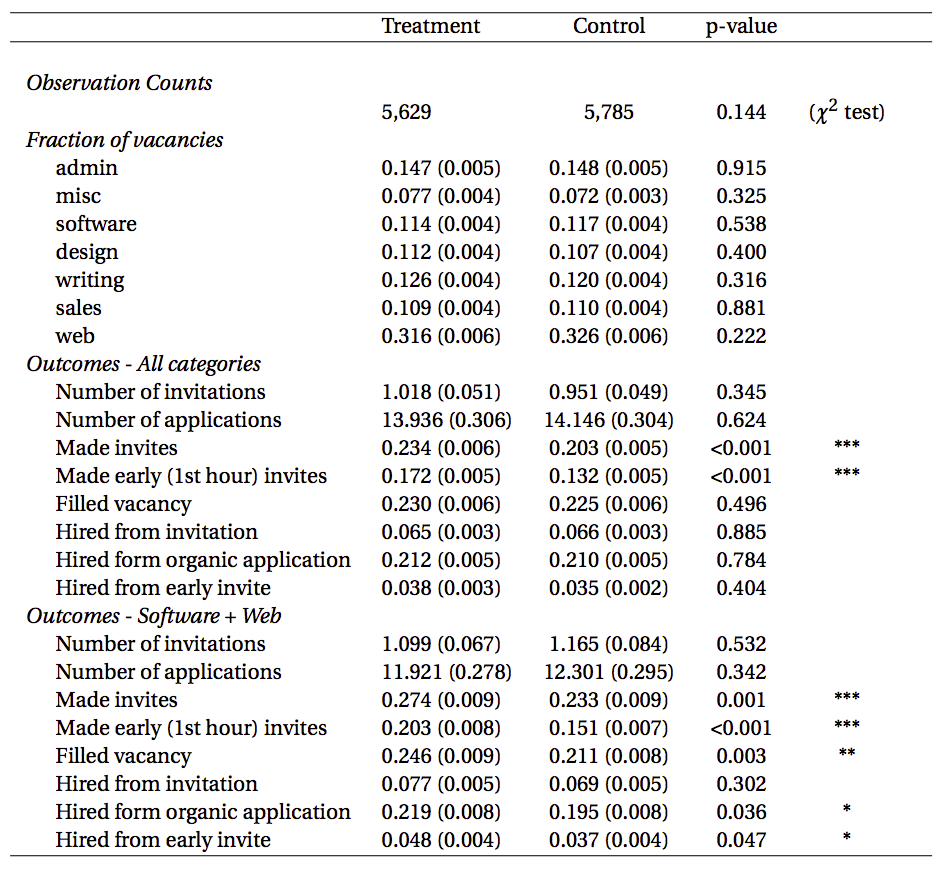
\includegraphics[width=0.9\textwidth]{present_dia5.png} \end{figure}
\end{minipage}
}

\nointerlineskip
\begin{tikzpicture}[remember picture,overlay]
\draw[line width=2pt,draw=red\isecond] (110pt, -40pt) rectangle (220pt,-100pt);
\end{tikzpicture}

\nointerlineskip
\begin{tikzpicture}[remember picture,overlay]
\draw[line width=2pt,draw=red\ithird] (22pt, -124pt) rectangle (245pt,-134pt);
\end{tikzpicture}

\nointerlineskip
\begin{tikzpicture}[remember picture,overlay]
\draw[line width=2pt,draw=red\ifourth] (22pt, -197pt) rectangle (245pt,-207pt);
\end{tikzpicture}

\nointerlineskip
\begin{tikzpicture}[remember picture,overlay]
\draw[line width=2pt,draw=red\ififth] (22pt, -212pt) rectangle (245pt,-230pt);
\end{tikzpicture}

\nointerlineskip
\putat{0.9}{0.3}{
\large
\textcolor{red\isixth}{Good}
}

\nointerlineskip
\putat{0.9}{0.36}{
\large
\textcolor{red\isixth}{balance}
}

\vspace{\textheight}

\end{minipage}
}
\end{animateinline}
\end{frame}

\begin{frame}
\begin{animateinline}[autoplay]{10}
\multiframe{5}{ii=0+25}{
\begin{minipage}{\textwidth}
\pgfmathtruncatemacro{\ifirst}{min(100,max(0,\ii))}%

\pgfmathsetmacro{\itrans}{\ifirst/100}%

\nointerlineskip
\putattrans{0.5}{0.5}{\itrans}{
\begin{minipage}{\textwidth}
\begin{figure}[H] \centering 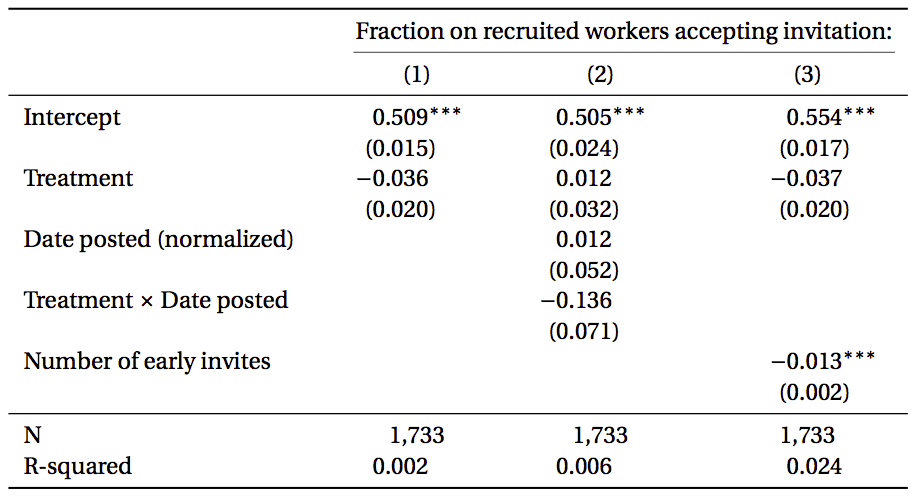
\includegraphics[width=\textwidth]{present_dia6.png} \end{figure}
\end{minipage}
}

\vspace{\textheight}

\end{minipage}
}
\end{animateinline}
\end{frame}

\begin{frame}
\begin{animateinline}[autoplay]{10}
\multiframe{5}{ii=0+25}{
\begin{minipage}{\textwidth}
\pgfmathtruncatemacro{\ifirst}{min(100,max(0,\ii))}%

\pgfmathsetmacro{\itrans}{\ifirst/100}%

\nointerlineskip
\putattrans{0.5}{0.5}{\itrans}{
\begin{minipage}{0.9\textwidth}
\begin{figure}[H] \centering 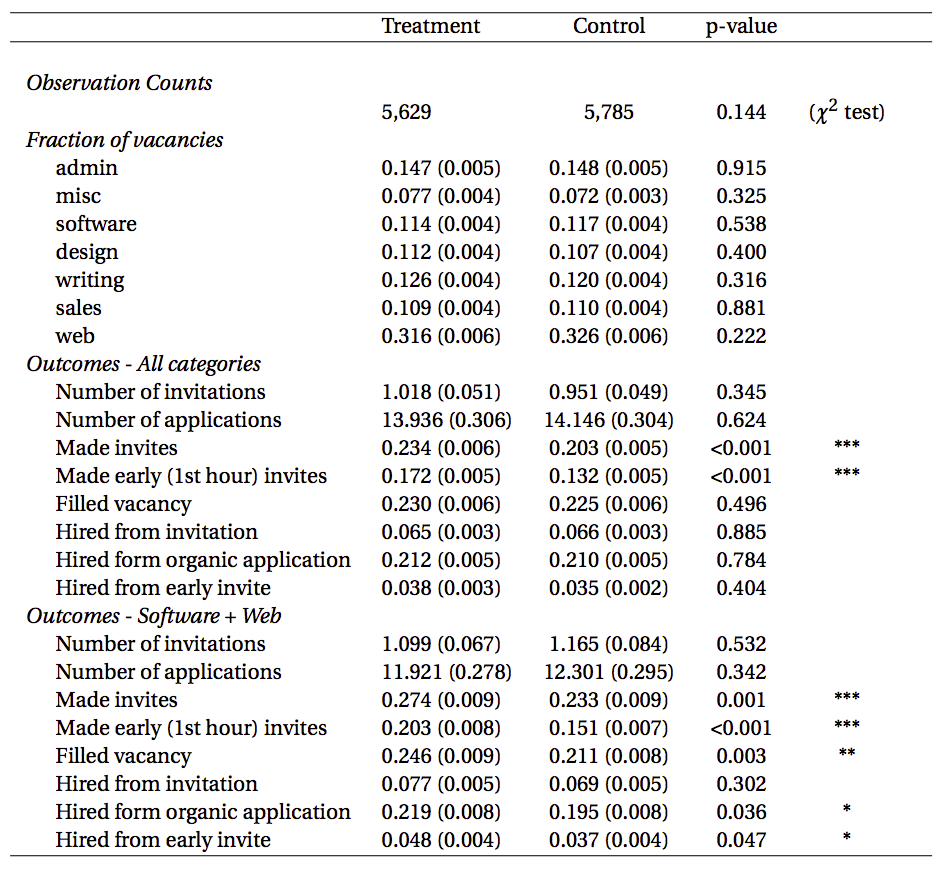
\includegraphics[width=0.9\textwidth]{present_dia5.png} \end{figure}
\end{minipage}
}

\vspace{\textheight}

\end{minipage}
}
\end{animateinline}
\end{frame}

\begin{frame}
\begin{animateinline}[autoplay]{10}
\multiframe{5}{ii=0+25}{
\begin{minipage}{\textwidth}
\pgfmathtruncatemacro{\ifirst}{min(100,max(0,\ii))}%

\pgfmathsetmacro{\itrans}{\ifirst/100}%

\nointerlineskip
\putattrans{0.5}{0.5}{\itrans}{
\begin{minipage}{\textwidth}
\begin{figure}[H] \centering 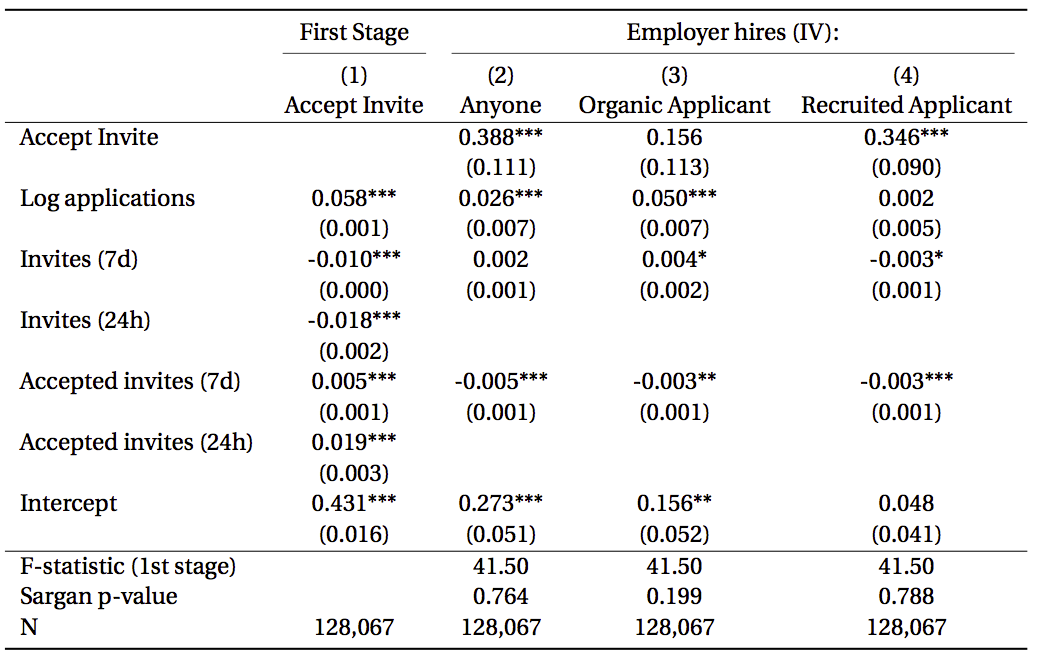
\includegraphics[width=\textwidth]{present_dia7.png} \end{figure}
\end{minipage}
}

\vspace{\textheight}

\end{minipage}
}
\end{animateinline}
\end{frame}

\begin{frame}
\begin{animateinline}[autoplay]{10}
\multiframe{5}{ii=0+25}{
\begin{minipage}{\textwidth}
\pgfmathtruncatemacro{\ifirst}{min(100,max(0,\ii))}%

\pgfmathsetmacro{\itrans}{\ifirst/100}%

\nointerlineskip
\putattrans{0.5}{0.5}{\itrans}{
\begin{minipage}{\textwidth}
\begin{figure}[H] \centering 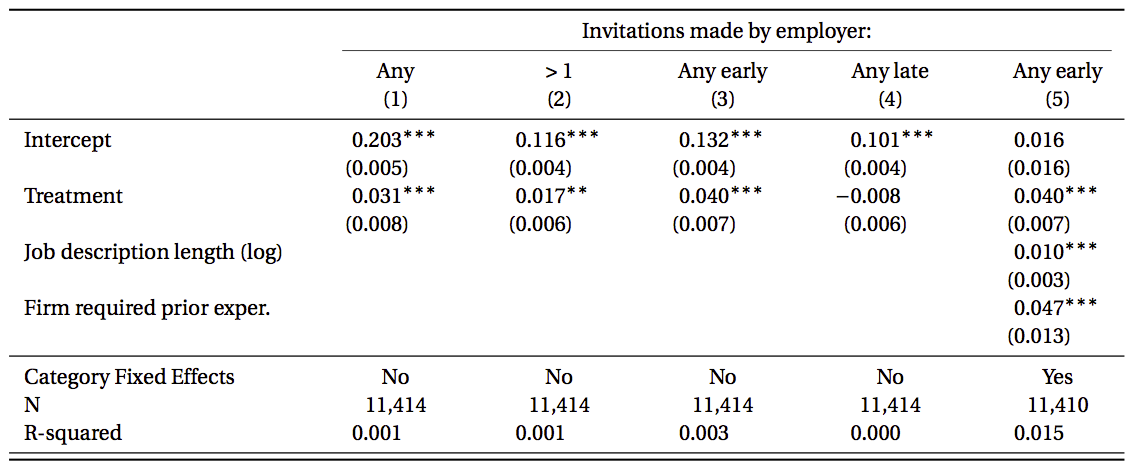
\includegraphics[width=\textwidth]{present_dia8.png} \end{figure}
\end{minipage}
}

\vspace{\textheight}

\end{minipage}
}
\end{animateinline}
\end{frame}

\begin{frame}{}
\begin{animateinline}[autoplay]{10}
\multiframe{5}{i=0+25}{
\begin{minipage}{\textwidth}
\begin{center}
\vspace{1mm}

\textcolor{gray\i}{Market design}

\textcolor{gray\i}{considerations}

\vspace{1mm}
\end{center}
\end{minipage}
}
\end{animateinline}
\end{frame}

\begin{frame}
\begin{animateinline}[autoplay]{10}
\multiframe{5}{ii=0+25}{
\begin{minipage}{\textwidth}
\pgfmathtruncatemacro{\ifirst}{min(100,max(0,\ii))}%

\pgfmathsetmacro{\itrans}{\ifirst/100}%

\nointerlineskip
\putattrans{0.5}{0.5}{\itrans}{
\begin{minipage}{\textwidth}
\begin{figure}[H] \centering 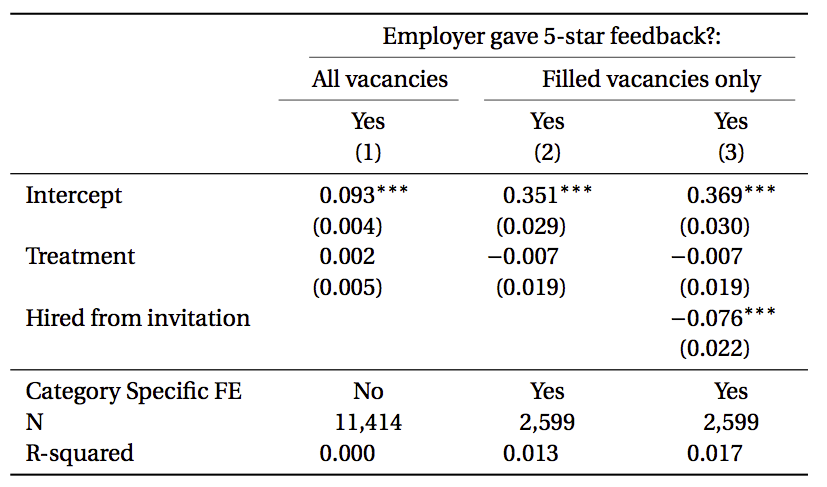
\includegraphics[width=\textwidth]{present_dia9.png} \end{figure}
\end{minipage}
}

\vspace{\textheight}

\end{minipage}
}
\end{animateinline}
\end{frame}

\begin{frame}{}
\begin{animateinline}[autoplay]{10}
\multiframe{5}{i=0+25}{
\begin{minipage}{\textwidth}
\begin{center}
\vspace{1mm}

\textcolor{gray\i}{Larger implications}

\vspace{1mm}
\end{center}
\end{minipage}
}
\end{animateinline}
\end{frame}

\begin{frame}{}
\begin{animateinline}[autoplay]{10}
\multiframe{5}{i=0+25}{
\begin{minipage}{\textwidth}
\begin{center}
\vspace{1mm}

\textcolor{gray\i}{Digitization of the}

\textcolor{gray\i}{supply side of the}

\textcolor{gray\i}{market}

\vspace{1mm}
\end{center}
\end{minipage}
}
\end{animateinline}
\end{frame}

\begin{frame}
\begin{animateinline}[autoplay]{10}
\multiframe{5}{ii=0+25}{
\begin{minipage}{\textwidth}
\pgfmathtruncatemacro{\ifirst}{min(100,max(0,\ii))}%

\pgfmathsetmacro{\itrans}{\ifirst/100}%

\nointerlineskip
\putattrans{0.5}{0.5}{\itrans}{
\begin{minipage}{\textwidth}
\begin{figure}[H] \centering 
\includegraphics[width=\textwidth]{present_dia10.png} \end{figure}
\end{minipage}
}

\vspace{\textheight}

\end{minipage}
}
\end{animateinline}
\end{frame}

\begin{frame}{}
\begin{animateinline}[autoplay]{10}
\multiframe{5}{i=0+25}{
\begin{minipage}{\textwidth}
\begin{center}
\vspace{1mm}

\textcolor{gray\i}{Back-up Slides}

\vspace{1mm}
\end{center}
\end{minipage}
}
\end{animateinline}
\end{frame}

\begin{frame}{}
\begin{animateinline}[autoplay]{10}
\multiframe{5}{i=0+25}{
\begin{minipage}{\textwidth}
\begin{center}
\vspace{1mm}

\textcolor{gray\i}{Employer FE Approach}

\vspace{1mm}
\end{center}
\end{minipage}
}
\end{animateinline}
\end{frame}

\begin{frame}
\begin{animateinline}[autoplay]{10}
\multiframe{5}{ii=0+25}{
\begin{minipage}{\textwidth}
\pgfmathtruncatemacro{\ifirst}{min(100,max(0,\ii))}%

\pgfmathsetmacro{\itrans}{\ifirst/100}%

\nointerlineskip
\putattrans{0.5}{0.5}{\itrans}{
\begin{minipage}{\textwidth}
\begin{figure}[H] \centering 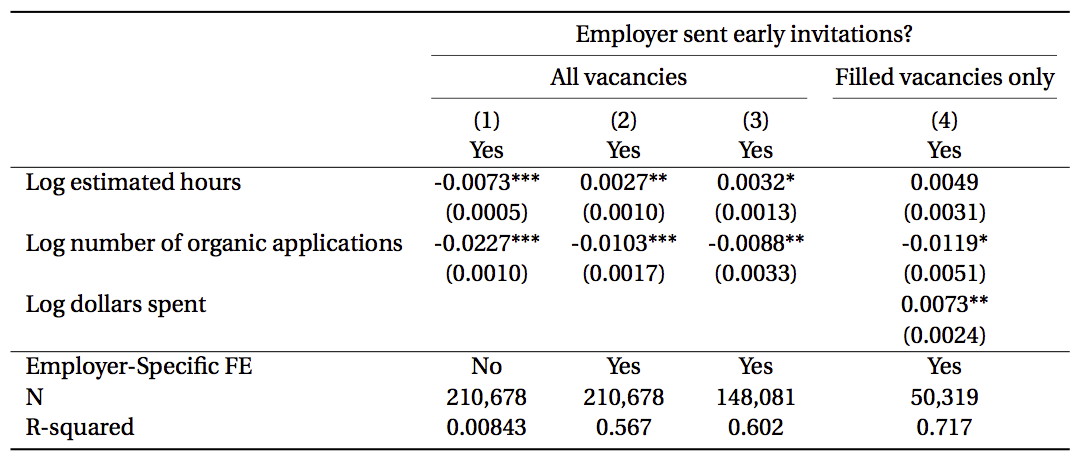
\includegraphics[width=\textwidth]{present_dia11.png} \end{figure}
\end{minipage}
}

\vspace{\textheight}

\end{minipage}
}
\end{animateinline}
\end{frame}

\begin{frame}
\begin{animateinline}[autoplay]{10}
\multiframe{5}{ii=0+25}{
\begin{minipage}{\textwidth}
\pgfmathtruncatemacro{\ifirst}{min(100,max(0,\ii))}%

\pgfmathsetmacro{\itrans}{\ifirst/100}%

\nointerlineskip
\putattrans{0.5}{0.5}{\itrans}{
\begin{minipage}{\textwidth}
\begin{figure}[H] \centering 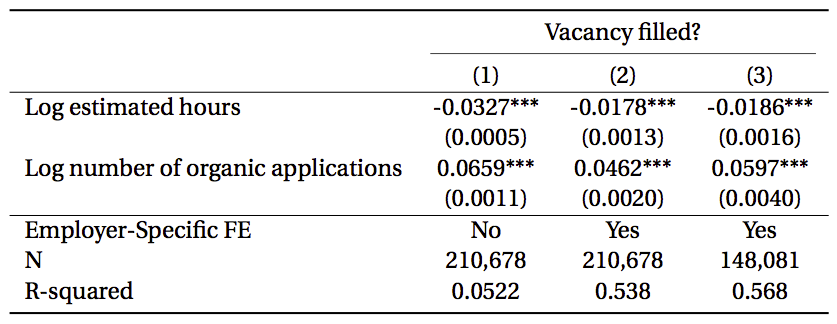
\includegraphics[width=\textwidth]{present_dia12.png} \end{figure}
\end{minipage}
}

\vspace{\textheight}

\end{minipage}
}
\end{animateinline}
\end{frame}

\begin{frame}
\begin{animateinline}[autoplay]{10}
\multiframe{5}{ii=0+25}{
\begin{minipage}{\textwidth}
\pgfmathtruncatemacro{\ifirst}{min(100,max(0,\ii))}%

\pgfmathsetmacro{\itrans}{\ifirst/100}%

\nointerlineskip
\putattrans{0.5}{0.5}{\itrans}{
\begin{minipage}{\textwidth}
\begin{figure}[H] \centering 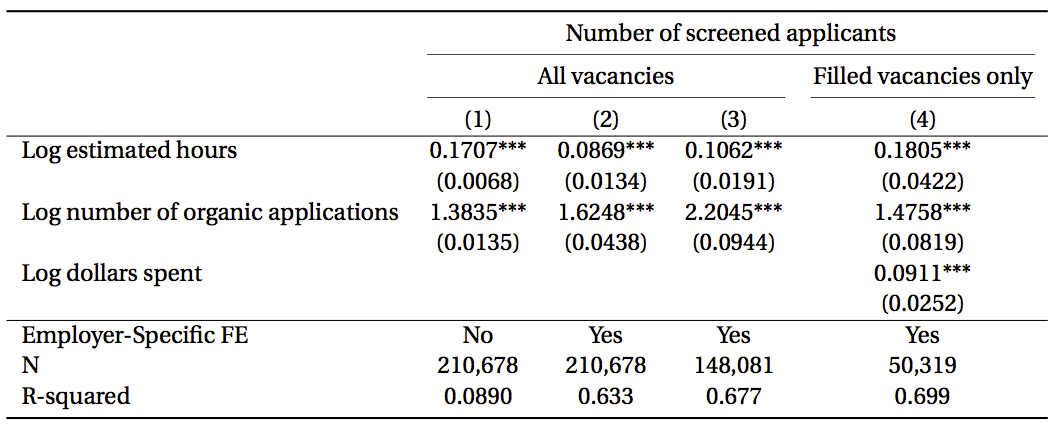
\includegraphics[width=\textwidth]{present_dia13.png} \end{figure}
\end{minipage}
}

\vspace{\textheight}

\end{minipage}
}
\end{animateinline}
\end{frame}

\begin{frame}
\begin{animateinline}[autoplay]{10}
\multiframe{5}{ii=0+25}{
\begin{minipage}{\textwidth}
\pgfmathtruncatemacro{\ifirst}{min(100,max(0,\ii))}%

\pgfmathsetmacro{\itrans}{\ifirst/100}%

\nointerlineskip
\putattrans{0.5}{0.5}{\itrans}{
\begin{minipage}{0.9\textwidth}
\begin{figure}[H] \centering 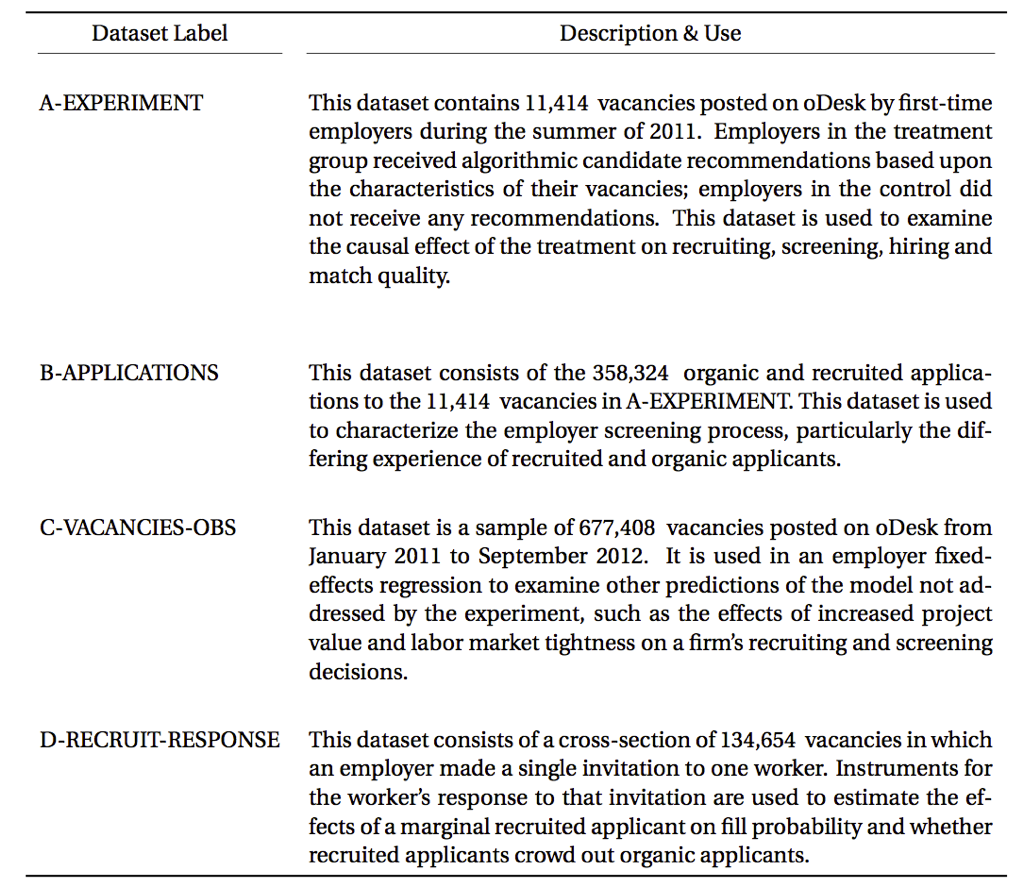
\includegraphics[width=0.9\textwidth]{present_dia14.png} \end{figure}
\end{minipage}
}

\vspace{\textheight}

\end{minipage}
}
\end{animateinline}
\end{frame}

\end{document}